\documentclass[degree=master]{thuthesis}
% 选项:
%   degree=[bachelor|master|doctor|postdoctor], % 必选
%   secret,                                     % 可选
%   pifootnote,                                 % 可选(建议打开)
%   openany|openright,                          % 可选,基本不用
%   arial,                                      % 可选,基本不用
%   arialtoc,                                   % 可选,基本不用
%   arialtitle                                  % 可选,基本不用

% 所有其它可能用到的包都统一放到这里了,可以根据自己的实际添加或者删除。
\usepackage{thuthesis}
\usepackage{algorithm2e}

% 定义所有的图片文件在 figures 子目录下
\graphicspath{{figures/}}

% 可以在这里修改配置文件中的定义。导言区可以使用中文。
% \def\myname{薛瑞尼}

\begin{document}

%%% 封面部分
\frontmatter
\thusetup{
  %******************************
  % 注意:
  %   1. 配置里面不要出现空行
  %   2. 不需要的配置信息可以删除
  %******************************
  %
  %=====
  % 秘级
  %=====
  secretlevel={秘密},
  secretyear={10},
  %
  %=========
  % 中文信息
  %=========
  ctitle={工业时间序列数据的特征学习\	\ 技术研究与应用},
  cdegree={工程硕士},
  cdepartment={软件学院},
  cmajor={软件工程},
  cauthor={胡志坤},
  csupervisor={邓仰东副研究员},
  %cassosupervisor={陈文光教授}, % 副指导老师
  %ccosupervisor={某某某教授}, % 联合指导老师
  % 日期自动使用当前时间,若需指定按如下方式修改:
   cdate={二〇一九年五月},
  %
  % 博士后专有部分
  cfirstdiscipline={计算机科学与技术},
  cseconddiscipline={系统结构},
  postdoctordate={2009年7月——2011年7月},
  id={编号}, % 可以留空: id={},
  udc={UDC}, % 可以留空
  catalognumber={分类号}, % 可以留空
  %
  %=========
  % 英文信息
  %=========
  etitle={Research and Application on Industrial Time Series Data Feature Learning},
  % 这块比较复杂,需要分情况讨论:
  % 1. 学术型硕士
  %    edegree:必须为Master of Arts或Master of Science(注意大小写)
  %             “哲学、文学、历史学、法学、教育学、艺术学门类,公共管理学科
  %              填写Master of Arts,其它填写Master of Science”
  %    emajor:“获得一级学科授权的学科填写一级学科名称,其它填写二级学科名称”
  % 2. 专业型硕士
  %    edegree:“填写专业学位英文名称全称”
  %    emajor:“工程硕士填写工程领域,其它专业学位不填写此项”
  % 3. 学术型博士
  %    edegree:Doctor of Philosophy(注意大小写)
  %    emajor:“获得一级学科授权的学科填写一级学科名称,其它填写二级学科名称”
  % 4. 专业型博士
  %    edegree:“填写专业学位英文名称全称”
  %    emajor:不填写此项
  edegree={Master of Engineering},
  emajor={Software Engineering},
  eauthor={Huang Fanling},
  esupervisor={Associate Research Fellow Deng Yangdong},
  %eassosupervisor={Chen Wenguang},
  % 日期自动生成,若需指定按如下方式修改:
  edate={May, 2018},
  %
  % 关键词用“英文逗号”分割
  ckeywords={时间序列,特征学习,符号回归,临界相变,生成式对抗网络},
  ekeywords={Time Series,Feature Learning,Symbolic Regression,Critical Transitions,Generative Adversarial Networks}
}
% 定义中英文摘要和关键字
\begin{cabstract}
  
  “工业4.0”的提出使大量工业数据得到有效的采集、传输和存储。其中时间序列数据是工业数据的重要表现形式,然而高维、高噪、时变等特性使其难以被开采利用。特征学习是数据得以有效利用的关键,一直是研究的热点和难点。本文主要针对时间序列数据的特征学习方法以及其在工业装备运维中的作用进行系统研究。首先针对以轴温为代表的设备正常运行数据,开展机理挖掘并实现状态估计;然后引入复杂系统临界相变理论,发现通用的失效早期预警特征并实现故障预测;最后基于生成式对抗网络,实现无监督式时间序列通用特征学习并支持分类任务。

  现有数据驱动的故障预测方法主要针对任务直接建模,缺乏对系统机理的认识。本文关注到基于符号回归的系统辨识方法具有系统结构表达能力。由此,利用以轴温为代表的设备正常运行数据展开研究,提出了基于符号回归的系统结构特征学习方法,并融合确定性优化算法和遗传算法完成训练,揭示了系统运行机理;进一步,本文将最优系统结构模型作为系统运行时的健康基线,设计了在线实时异常检测框架。此工作在一定程度上弥补了现有方法的不足。

  工业系统的故障数据普遍存在小样本、不完备的特性。现有系统失效特征学习方法大多针对特定系统建模,普适性较差。本文提出了基于复杂系统临界相变理论的早期预警特征学习方法,首先挖掘时间序列的随机波动信号,然后在此基础上学习失效早期预警特征,接下来通过多种方法检验系统失效与临界相变的一致性。最后针对早期预警特征,本文提出了关键跳变检测算法实现故障预测。利用 4 种不同类型的工业数据集展开实验,证明了方法的有效性和通用性。此工作为研究通用方法来预测由工业系统失效引起的潜在灾难提供了新视角。

  工业时间序列标记数据获取难的问题严重限制了监督式学习方法的应用。生成式对抗网络(Generative Adversarial Nets, GAN)是实现无监督式学习的新道路,但鲜有针对时间序列的模型。本文提出了时间序列生成式对抗网络(Time Series GAN,TSGAN),并以无监督的方式完成训练,利用85个公开的时间序列数据集展开实验。一方面,TSGAN 的生成器学习了真实数据集的分布,并生成逼真的多样化的时间序列;另一方面,将TSGAN的判别器作为特征转换器与简单分类器结合构建了半监督式分类框架,并取得优秀效果。此工作为无监督式时间序列特征学习以及基于此的半监督式学习提供了新思路。


\end{cabstract}

% 如果习惯关键字跟在摘要文字后面,可以用直接命令来设置,如下:
% \ckeywords{\TeX, \LaTeX, CJK, 模板, 论文}

\begin{eabstract}

The proposal of "Industry 4.0" enables a large number of industrial data to be effectively collected, transmitted and stored. Time-series data is the most significant resource to reflect the performance of operating industrial systems. However, it is hard to utilize time-series data because of its characteristics of high dimension, heavy noise and time variance. It has always been a challenging but active research subject to learn valuable features from messy time-series data. This thesis mainly studies time-series feature learning and its role in the maintenance of industrial equipments. Firstly, aiming at the normal running data of equipments represented by bearing temperature, mechanism mining is carried out and accurate state estimation is realized. Secondly, the critical transition theory of complex systems is introduced to discover the common early warning features of failure and support the realization of fault prognostics. Finally, based on the generative adversarial network (GAN), the unsupervised time-series general feature learning model is proposed and further supports the classification task. 

The existing data-driven fault prognostics methods are mainly aimed at direct modeling of tasks and lack understanding of the system mechanism. This thesis focuses on the symbolic regression based system identification, which has the ability to distill the mathematical equation from the data directly. Therefore, the normal running data of equipments represented by bearing temperature was used to carry out the research, a framework based on symbolic regression was proposed for system structure feature learning, and deterministic optimization algorithm and genetic algorithm were combined to conduct the training process. The structure feature revealed the system mechanism and the interaction relationship among signals. Furthermore, the optimal structure model was used as the health baseline to support the design of an online real-time anomaly detection framework. This work has made up for the shortcomings of the existing methods to some extent.

The failure data of industrial systems generally has the characteristics of small sample and incompleteness. Most of the existing methods of system failure feature learning are aimed at specific systems and have poor universality. This thesis proposed an early warning feature learning method based on the critical transition theory of complex systems. Firstly, the inherent random fluctuation signals of time-series were mined, and based on this, the early warning feature of failure was learned, then the consistency between system failure and critical transition were verified by various methods. Finally, this thesis proposed a key jump detection algorithm to make use of early warning feature to realize fault prognostics. Experiments were carried out on four different types of industrial data sets, which proved the universality and effectiveness of the method. Such a discovery gives a new perspective towards a generic methodology to predict and prevent potential disasters caused by the failure of industrial systems. 

The difficulty in obtaining industrial time-series labelled data seriously limits the application of supervised learning methods. GAN is a new way to realize unsupervised learning, but there are few models for time-series. In this thesis, Time-Series GAN (TSGAN) was proposed and the training process was conducted in an unsupervised way. Experiments were carried out using 85 benchmark time-series datasets. On one hand, the generator of TSGAN can effectively learn the distribution of time-series datasets and generate realistic and diversified time-series. On the other hand, the discriminator of TSGAN as a feature encoder was combined with simple classifiers to form a semi-supervised time-series classification framework, which gains excellent result. This work provides a new idea for unsupervised time-series feature learning and semi-supervised machine learning based on it.

\end{eabstract}

% \ekeywords{\TeX, \LaTeX, CJK, template, thesis}

% 如果使用授权说明扫描页,将可选参数中指定为扫描得到的 PDF 文件名,例如:
% \makecover[scan-auth.pdf]
\makecover

%% 目录
\tableofcontents

%% 符号对照表
%\begin{denotation}[3cm]
\item[HPC] 高性能计算 (High Performance Computing)
\item[cluster] 集群
\item[Itanium] 安腾
\item[SMP] 对称多处理
\item[API] 应用程序编程接口
\item[PI] 聚酰亚胺
\item[MPI] 聚酰亚胺模型化合物,N-苯基邻苯酰亚胺
\item[PBI] 聚苯并咪唑
\item[MPBI] 聚苯并咪唑模型化合物,N-苯基苯并咪唑
\item[PY] 聚吡咙
\item[PMDA-BDA]	均苯四酸二酐与联苯四胺合成的聚吡咙薄膜
\item[$\Delta G$] 活化自由能 (Activation Free Energy)
\item[$\chi$] 传输系数 (Transmission Coefficient)
\item[$E$] 能量
\item[$m$] 质量
\item[$c$] 光速
\item[$P$] 概率
\item[$T$] 时间
\item[$v$] 速度
\item[劝学] 君子曰:学不可以已。青,取之于蓝,而青于蓝;冰,水为之,而寒于水。木
  直中绳。輮以为轮,其曲中规。虽有槁暴,不复挺者,輮使之然也。故木受绳则直,金就
  砺则利,君子博学而日参省乎己,则知明而行无过矣。吾尝终日而思矣,不如须臾之所学
  也;吾尝跂而望矣,不如登高之博见也。登高而招,臂非加长也,而见者远;顺风而呼,
  声非加疾也,而闻者彰。假舆马者,非利足也,而致千里;假舟楫者,非能水也,而绝江
  河,君子生非异也,善假于物也。积土成山,风雨兴焉;积水成渊,蛟龙生焉;积善成德,
  而神明自得,圣心备焉。故不积跬步,无以至千里;不积小流,无以成江海。骐骥一跃,
  不能十步;驽马十驾,功在不舍。锲而舍之,朽木不折;锲而不舍,金石可镂。蚓无爪牙
  之利,筋骨之强,上食埃土,下饮黄泉,用心一也。蟹六跪而二螯,非蛇鳝之穴无可寄托
  者,用心躁也。—— 荀况
\end{denotation}



%%% 正文部分
\mainmatter
% !TEX root = ../main.tex

\chapter{绪论}
\label{cha:intro}


\section{研究背景与意义}
\label{sec:meaning}
% 挑战 --- 工业转型对工业系统安全性的要求越来越高。
"工业4.0"的概念在2013年被正式提出之后,“智能化”随即成为引领第四代工业革命的主题,各国纷纷制定政策以做好准备迎接工业转型的挑战与机遇。2011年在德国汉诺威工业博览会上“工业4.0”的概念首度被三位教授提出。2013年4月在汉诺威工博会上《保障德国制造业的未来:关于实施“工业4.0”战略建议书》发布,至此,“工业4.0”成为《德国2020高技术战略》的十大未来项目之一并正式上升为国家战略。\cite{kagermann2013recommendations}。美国随后颁布了《先进制造业合作伙伴》战略\cite{advanced2012capturing}。我国政府颁布了以实现制造强国为战略目标的《中国制造2025》政策\cite{周济2015智能制造——“中国制造}。随着工业转型,更智能化的工业系统在国家基础建设和发展进程中将扮演更重要的角色,安全问题不容忽视,《中国制造2025》中“质量为先”的基本方针更是充分体现了安全问题在工业转型中的重要性。

% 挑战 ---工业现场安全可靠的要求
工业生产的顺利进行是维护国民经济和生活保障的重要基础,保证工业生产现场和工业装备运行现场安全可靠的运行至关重要。工业生产和工业装备的安全问题,既是企业产品质量的重要标志,也是全社会关注的重点。1984年设在印度博帕尔市的美国联合炭化物公司开办的一家农药厂发生的毒气泄漏事故(死亡2500人,中毒125000人)、1986年两起震惊世界的巨大事故(美国“挑战者”号航天飞机爆炸和前苏联切尔诺贝利核电站爆炸事故)等,使人们对安全问题有了更加深入的认识\cite{工业安全评价方法与矿井安全评价技术综述}。以铁路为例,随着我国铁路提速和基础设施技术改造,列车的运行速度和密度日益增大,铁路运输生产的系统复杂度和风险度显著提高。为了适应现代生产生活发展的需要,企业安全监察部门应当尽可能的建立起安全预警系统,实现安全管理模式由“事故出发型”向“事故发现型”的转变\cite{铁路安全预警系统的研究与涉及}。保证复杂的工业系统可靠、安全、可持续的运行面临巨大的挑战。

% 机遇 ---- 监控设备的发展,深度学习技术的成熟,嵌入式设备的进步
随着社会的进步和科技的发展,视频监控也经历者从模拟化向数字化、网络化、智能化的革命,通过视频监控系统就能够快速、实时的进行监控和监视。
视频图像分析技术作为智能监控系统的核心技术,正广泛应用于公共安全监控领域。随着以摄像机为核心的视频监控系统成本日益降低,视觉监控系统在我国开始步入普及阶段。人脸识别在监控系统中发挥了重要作用因为它不需要其他物体的协助\cite{face2012recoginition}。视频和图像数据是人们体验最直观的数据类型,可以从图像中获取高层次的信息,比如通过观察列车受电弓接触点位置可以得知受电弓接触网是否接触良好后者存在脱网等安全隐患,通过观察列车驾驶员的操作动作得知操作的规范性和驾驶员的技术水平。

近年来对着深度学习技术的火热发展,图像数据的目标检测算法也从基于手工特征的传统算法转向了基于深度学习的检测算法\cite{deeplearing2018survey}。深度学习技术和图像检测算法的发展使得对工业现场的图像进行可靠高效的分析成为可能。而在硬件方面,嵌入式处理器的计算能力不断提升,已经广泛地应用于我们生活的各个领域,例如:计算机,汽车,航天飞机等。

% 挑战 --- 视频安全监控
但是在工业生产现场,视觉监控系统的功能仅仅停留在检查人员对视频信号的人工监视和事后录像分析上,并没有充分利用目前计算机技术告诉发展所提供的智能算法和强大的计算能力\cite{面向视觉监视实时跟踪的动态背景更新方法}。工业生产现场的视频监控系统迫切需要对危险状态进行线实时的分析,以实现对生产运行环境的可知可控。从视频监控系统采集的图像中利用深度学习技术学习检测风险是实现生产环境隐患实时监测的核心环节,然而工业图像普遍存在像素低,信噪比低的特点,导致标注难和分析难的问题;再者工业系统运行时故障属于小概率事件,鲁棒的图像检测算法需要不断的对新产生的数据进行学习分析,需要设计能够对不断产生的监控数据在线学习的算法,才能保证日后的检测任务中保证有效性。工业生产的危险预警重点在于及时预测,基于深度学习的模型通常需要大量的计算和内存访问,嵌入式处理器的计算能力相对较差,需要对深度学习模型进行压缩优化,得到最佳的网络结构,最终可以在嵌入式设备中实时运行。
如果能利用视频监控系统监控工业生产现场的状态,并对监控的视频数据进行实时分析,那么工业生产现场及设备一旦出现危险状况,可以及时预警处理,避免重大的生命财产损失。

综上所述,本文主要研究工业图像检测算法,并将检测模型进行压缩优化,最终在工业现场的嵌入式设备达到实时检测的要求,同时利用现场不断采集的新数据进行模型的自我学习更新,以适应工业现场复杂多变的特点。因此本文的研究对于基于图像数据及时检测工业生产现场的危险状态,发现并预测潜在故障隐患,建立依靠先进技术支撑的故障预警系统,具有重大意义。

\section{研究内容与贡献}
\label{sec:content-contribution}

%突出我的方法相对于传统方法的先进性。理论贡献,公开benchmark,在实验室的列车故障数据上进行验证,具有现实意义
\subsection{研究内容}
本文针对复杂多变的工业图像的检测算法及其加速技术展开系统研究。首先论述了研究的北京和意义,然后然后梳理并综述相关研究工作。接下来针对3个现实问题依次展开工业图像检测算法研究与应用的工作:(1)针对复杂的工业现场图像数据,以及现有的图像检测算法只对单张图像独立分析的问题,提出预测式的图像检测算法,结合前序图像的状态的估计值和当前图像的预测值,对该时刻的图像状态进行估计,并在列车受电弓数据上展开对比实验;(2)针对工业现场的监控数据不断更新,情况复杂多变的挑战,以及基于深度学习的模型训练周期长,需要定期更新的问题,提出基于当前模型恒等变换的在线训练方法,该方法快速的将小模型的知识迁移到新的模型,并且不断对新的数据进行学习。(3)而基于深度学习的图像检测模型参数量和计算量通常较大,在嵌入式设备中无法实时运行的问题,提出通过对卷积神经网络进行剪枝来搜索最佳的网络结构,极大的加快了检测效率。最后进行总结与展望。

论文的主要研究内容和结构安排如下:

第 1 章:绪论
	
首先论述研究背景和意义;其次介绍本文主要研究内容和贡献。

第 2 章:相关研究综述

对相关内容研究,深度学习、图像检测算法,训练加速算法、卷积神经网络剪枝、嵌入式系统、以及模型移植等,进行梳理和综述;论述现有工作的优缺点以及与本文工作的契合点。

第 3 章:基于深度学习的预测式工业图像检测算法

针对工业视频和图像场景复杂的挑战,以及现有图像检测算法无法利用前序图像信息的问题,本文利用以列车受电弓图像为代表的工业图像数据进行研究实验。首先介绍研究背景与数据分析工作;然后提出基于深度学习方法和前序图像的预测式图像检测算法,并进行对比实验分析。

第 4 章:基于模型恒等变换的在线训练算法

针对工业现场的监控数据不断更新,情况复杂多变的挑战,以及现有的深度学习模型训练方法大多是利用采集好的数据从零开始训练,模型更新周期长的问题。本文提出基于模型恒等变换的在线训练方法,首先对当前模型结构加宽加深得到新的模型结构,同时不改变模型的映射关系,利用不断采集的新数据对新的模型进行微调,最后在2个公开的图像数据集上进行对比实验分析。

第 5 章:基于剪枝搜索的深度模型嵌入式移植优化算法

针对而基于深度学习的图像检测模型参数量和计算量较大的挑战,目前难以在嵌入式设备中实时运行。本文针对工业现场常用的ARM平台,首先进行卷积核的剪枝探索最优的网络结构,接下来逐层测试卷积神经网络前向传递过程的计算时间和内存访问时间,最终得到最佳的网络结构。

第 6 章:总结与展望

对本文工作以及相关结论进行概要总结;对未来工作进行展望。

\subsection{研究贡献}

1.本文基于以列车受电弓监控图像为代表的工业图像数据,提出基于深度学习方法和前序图像的预测式图像检测算法,进一步利用前序图像的状态信息对当前时刻的图像进行检测,在一定程度上弥补了现有连续图像检测算法的不足。

2.本文提出基于模型恒等变换的在线训练方法,该方法快速的将小模型的知识迁移到新的模型,缩短新模型的训练时间。本文在2个的图像数据集展开实验,证明该方法的有效性。

3.本文提出基于剪枝搜索的深度模型嵌入式移植优化算法,对卷积核剪枝以探索最优的网络结构,并在ARM平台台逐层测试卷积神经网络前向传递过程的计算时间和内存访问时间,最终得到最佳的网络结构。

4.本文所有方法均得到了真实场景数据或公开数据的验证,具有较好的应用价值和借鉴意义。



\chapter{相关研究综述}
\label{cha:review}

\section{故障预测与健康管理}
\label{sec:review-phm}

% 如图\ref{fig:phm-maintenance}所示故障维修体制发展至今可划分为三个时期,即事后维修(又称无计划维修)、计划性维修和视情维修\cite{jardine2006review}。早期工业系统复杂性和安全性要求较低,采用事后维修即可满足需求。随着安全性需求不断提升,维修体制逐渐向计划维修过渡,即对系统进行定期检查、保养和维修以延长系统寿命、降低系统故障风险。社会工业科技不断进步,系统集成度越来越高、复杂性不断增加,劳动密集型的计划维修体制费时费力、效率低下,维修成本不断攀升以至于已经成为很多工业公司的主要支出\cite{peng2010current}。在此背景下,维修技术逐渐过渡到高效的视情维修\cite{jardine2006review,peng2010current}。视情维修主要由数据获取、数据处理和维修决策三个步骤组成,基于获取的数据以数据处理为手段挖掘潜在价值实现系统故障诊断和预测,进而作出是否采取维修行为的决策。视情维修很大程度避免了计划维修中非必要的维修投入。
% \begin{figure}[H]{}
% \centering
% 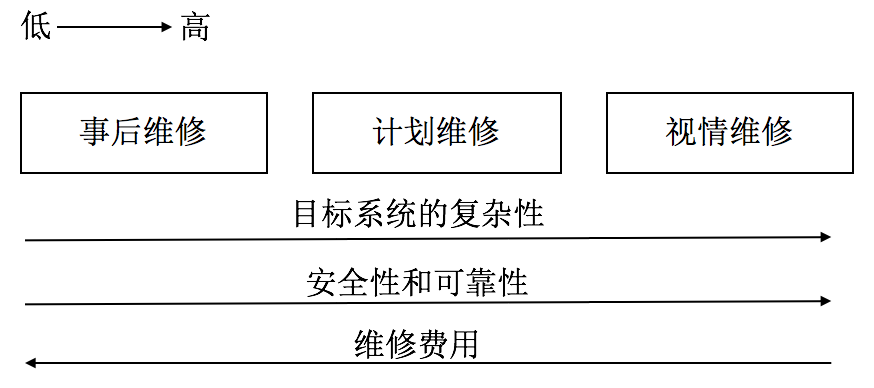
\includegraphics[scale=0.5]{figures/phm-maintenance.png}
% \caption{维修体制进化路线}
% \label{fig:phm-maintenance}
% \end{figure}
故障预测与健康管理(PHM)技术是实现视情维修的有效手段,是利用大数据技术和机器学习技术,把失效机制、寿命预测和全生命周期管理整合在一起进行统筹化的系统工程\cite{lee2014prognostics}。本文将PHM系统工程的主要内容归纳为图\ref{fig:phm-framework}。目前在国外尤其是美国 PHM 系统已投入应用,比如美军的 F-35 战斗机已全面部署 PHM 系统,取消计划性检修,大大降低了系统维修开销\cite{brown2007prognostics}。PHM 技术的有效性得到验证后倍受关注,正迅速覆盖除军事以外的民用技术领域,比如 民航、交通、船舶、制造业等领域。相比之下,国内的PHM技术正处于起步阶段,研究主要基于航空航天、船舶等高技术复杂装备展开\cite{彭宇2010故障预测与健康管理技术综述},大部分复杂工业系统仍沿用计划维修体制。因此,如何利用 PHM 技术实现中国维修体制的转型仍是一个亟待解决的问题。
\begin{figure}[H]
\centering
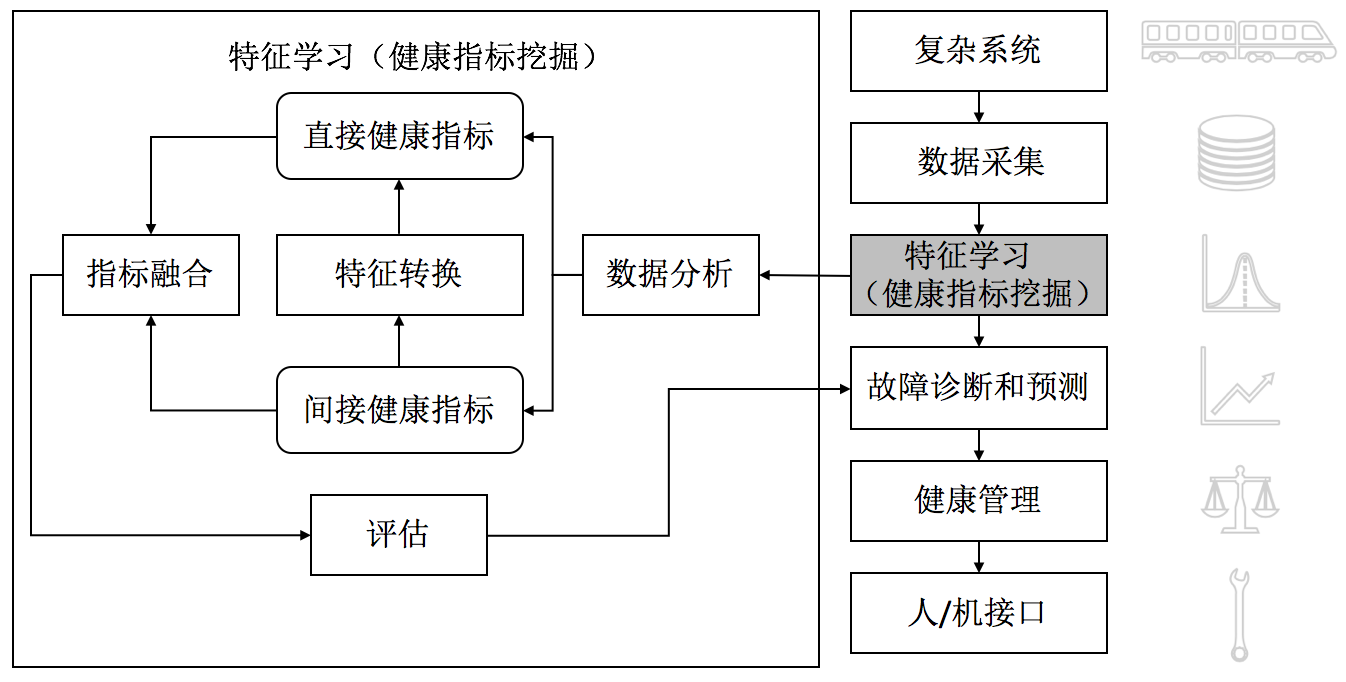
\includegraphics[scale=0.5]{figures/phm-framework.png}
\caption{PHM 系统工程}
\label{fig:phm-framework}
\end{figure}
故障预测是 PHM 的核心要义,其划分大同小异,比如Si 等人将故障预测方法分为四类,即基于实验的、数据驱动的、基于物理模型的和混合的故障预测方法\cite{si2011remaining};Lee 等人划分为三类,即基于模型的、数据驱动的和混合的故障预测方法\cite{lee2014prognostics};彭宇等人分为三类,即基于模型的、数据驱动的和基于统计可靠性的故障预测方法\cite{彭宇2010故障预测与健康管理技术综述};Pecht 等人分为两类,即基于模型的和数据驱动的故障预测方法\cite{pecht2010prognostics}。为便于讨论和研究,本文统一将故障预测方法划分为以下两类:

1. 基于模型的故障预测方法:基于模型的故障预测方法依赖精确的物理模型和专家知识建模,通过对比观测数据与内置精确模型仿真数据的差异来发现和预测故障。比如Byington 等人采用基于模型的故障预测方法实现飞机控制部件的故障预测,需要配置精确的物理模型实现参数估计\cite{byington2004model}。由于有精确的物理模型为基础,基于模型的故障预测方法预测精度最高。然而在全球化趋势下获得清晰准确的机理知识困难甚至不可能。因此,基于模型的故障预测方法应用领域较窄,局限于系统机理透明并且对精度要求很高的领域,如军用装备领域。

2. 数据驱动的故障预测方法:数据驱动的故障预测方法采用数据挖掘和机器学习技术,从历史运行数据中提取系统健康指标,并实现故障诊断和预测。比如获得PHM-2008竞赛冠军的 Wang 等人\cite{wang2008similarity},首先分析历史数据找到反应系统性能的关键信号,然后基于关键信号采用线性回归方法构建系统健康指标,最后使用基于相似性的分类方法实现系统剩余寿命预测。数据驱动的故障预测方法预测不依赖准确的机理知识,具有良好的灵活性便于实际应用,然而现有方法大多针对任务直接建模,缺乏对系统机理的认识。

工业大数据技术的成熟使数据驱动的故障预测方法倍受青睐\cite{tsui2015prognostics,si2011remaining},有少部分学者还提出混合模型的概念尝试融这两类模型的优点来提升故障预精度\cite{pecht2010prognostics}。针对工业系统采集的数据可分为事件数据和状态监测数据两类,其中状态监测数据是反应系统性能的最好依据,按数据类型可分为实值数据(比如温度、湿度等)、波形数据(比如震动信号、声学信号等)和多维数据(比如图片等)\cite{jardine2006review}。基于获取方式的不同,状态监测数据又可进一步分为直接状态监测数据和间接状态监测数据两类。由此衍生两大类数据驱动的故障预测方法,分别为基于直接状态监测数据的故障预测方法和基于非直接监测数据的故障预测方法\cite{si2011remaining}。

对于数据驱动的故障预测方法,如何有效的处理数据并挖掘具有反应系统状态变迁能力的特征或指标是关键,这一过程通常被称为健康指标(简称指标)提取\cite{pecht2010prognostics}。本文将健康指标提取过程以及其在PHM系统工程中所扮演的角色归纳为图\ref{fig:phm-framework}。系统健康指标可以分为以下两类\cite{zhou2011latent}:(a)直接指标,直接与系统失效机理相关,比如刹车片的厚度、齿轮裂纹深度等;(b)非直接指标,部分反应系统失效机理,如分析石油数据提取的特征。直接指标更难获取,但可以更精确反映系统的健康状态。非直接指标可通过特征转换的方式映射为直接指标\cite{si2011remaining,zhou2011latent}。


健康指标挖掘已得到广泛关注和研究。
Yan 等人,针对电梯门运动系统,通过逻辑斯蒂回归(Logistics Regression, LR)从多维数据中提取单维健康指标,并基于此利用ARMA实现剩余寿命预测\cite{yan2004prognostic}。
Wang 等人,针对涡扇发动机系统,以数据分析为基础从20多维传感器信号中找到与失效密切相关的6维关键信号,基于此通过线性回归构建单维系统健康指标,最后利用健康指标实现剩余寿命预测\cite{wang2008similarity}。
Patil 等人通过实验发现绝缘栅双极型晶体管(Insulated Gate Bipolar Transistors, IGBTs)的3个失效敏感信号可作为系统健康指标提取的基础\cite{patil2008failure}。
Zhou 等人指出状态空间模型提供了从非直接指标到直接指标的有效估计,针对现有状态空间模型高度依赖离散时间、离散状态、直线性和高斯性等假设的局限性,提出了一种不依赖以上假设的状态空间模型并采用基于蒙特卡罗的算法实现模型参数估计和剩余寿命预测,最后通过MATLAB进行数值仿真实验\cite{zhou2011latent}。
He 等人,针对齿轮震动信号,通过基于柯列斯分解的转换从多维相关震动信号中提取单维的反映系统健康状态的指标,并在此基础上利用滑动平均模型(Auto-Regressive and Moving Average Model, ARMA)实现剩余寿命预测\cite{he2012integrated}。
Liu 等人,针对锂离子电池系统,提出并设计了完整的健康指标提取框架,主要涉及数据转换、相关性分析、健康指标评估几个阶段\cite{liu2015health}。 

综上所述,健康指标挖掘是数据驱动的PHM方法的核心。然而现有的健康指标挖掘方法大多针对特定场景和系统部件进行建模设计,局限性较大,很难进行广泛应用。再者大多健康指标虽具有预测能力,但缺乏对系统底层机理的良好解释。针对以上问题,本文将结合物理系统动力学特性、复杂系统临界相变理论和机器学习技术,以数据驱动的方法为主要手段,同时充分利用可获取的先验知识,探索新方法从高维、高噪、时变的工业时间序列中挖掘反应系统状态变迁和运行机理的普适特征。另外本文将健康指标挖掘统称为{\heiti 特征学习}。

%\subsection{时间序列数据分析和特征学习方法}
\section{时间序列特征学习}
\label{sec:ts-representation-review}
% 时间序列的普遍性和重要性
% 时间序列的定义
% 时间序列分析的一般流程:数据采集 + 预处理 + 特征学习 + 任务
% 本文主要研究:预处理和特征学习,详细讨论
% 时间序列数据预处理方法:主要参考两本书
% 时间序列特征学习方法:按照现有分类进行概述

时间序列是普遍存在的重要数据类型,比如生态领域随时间变化的种群数量、金融领域随时间波动的经济指标、医疗领域随时间变化的生理指标、工业系统领域随时间变化的状态监测数据等都是时间序列\cite{aggarwal2015data}。一般的,时间序列数据由随时间变化的连续过程的采样点构成,是生态、金融、医疗和工业等领域的重要资源\cite{esling2012time,gaber2005mining}。

时间序列存在高维、高噪、时变等特点使其难以被开采利用,时间序列分析被认为是数据挖掘领域最具挑战的十个问题之一\cite{langkvist2014review}。对时间序列的开采过程通常可称为信号处理(Signal Process)\cite{rabiner1975theory}、时间序列分析(Time Series Analyais)\cite{bisgaard2011time}或时间序列挖掘(Time Series Mining)\cite{fu2011review}。从信号处理的角度,大多时间序列为电信号,比如震动信号、脑电波等,因此有很多时间序列开采方法都源于信号分析学,比如常见的傅立叶变换、正弦变换、余弦变换等信号转换方法,高通滤波、低通滤波、卡尔曼滤波等可以有效消除噪音影响的滤波方法。从时间序列分析的角度,大多方法倾向于分析时间序列的统计特性,比如时间序列的稳定性、自相关性等,应用场景多为时间序列预测。从时间序列挖掘的角度,更多强调利用数据挖掘和机器学习方法来对时间序列进行开采利用,应用场景除了传统的预测任务外还关注索引、分类、聚类、主题挖掘等任务\cite{fu2011review}。

本文统一采用{\heiti 时间序列挖掘}这一术语表示对时间序列数据的开采利用过程,关键流程归纳为图\ref{fig:tsm-framework},主要包含数据采集、特征学习及应用三个环节。其中,特征学习是数据得以有效利用的关键,一直是研究热点和难点\cite{langkvist2014review}。

\begin{figure}[H]
\centering
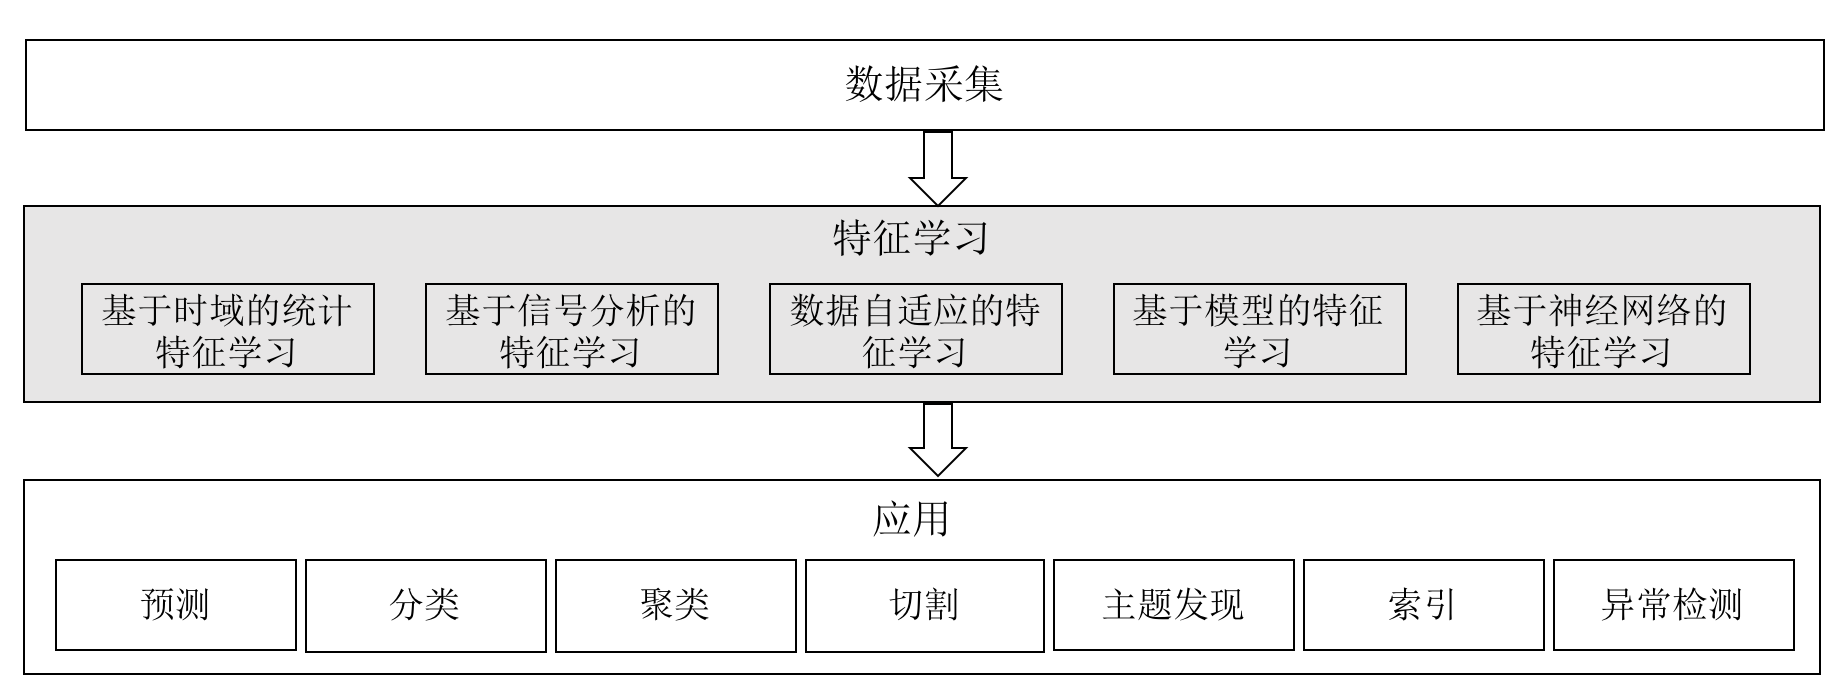
\includegraphics[scale=0.45]{figures/tsm-framework.png}
\caption{时间序列挖掘流程}
\label{fig:tsm-framework}
\end{figure}

\subsection{时间序列数据采集}

%“工业 4.0”的提出使工业数据得到有效的采集、传输和存储\cite{manyika2011big}。
工业数据主要通过传感器进行采集,为保证数据质量,此过程通常需要进行适当的预处理操作。

(1)数据集成

数据集成是指整合位于不同资源上的数据并为用户提供统一视图的过程\cite{lenzerini2002data}。在工业系统中,数据往往存放于不同数据库,再者不同系统、同一系统的不同部件的采样配置通常也有差异,因此数据集成是保证数据一致性的重要手段。
%最典型的不同采样率的时间序列数据需要进行时间对标以保证不同来源的观测值在时间上是一致的。

(2)重采样

采样率是时间序列数据采集过程的关键参数,并且因应用场景不同通常存在较大差异,因此不同来源的时间序列需进行时间对标以确保数据的一致性。此外过高的采样率容易导致冗余,而过低的采样率容易导致关键信息丢失。因此,在针对时间序列展开深入挖掘之前,通常先根据任务需求对数据进行上采样或下采样处理。上采样一般通过插值方法实现,下采样一般通过数据规约实现。处理信号数据时重采样往往会与滤波操作结合。更具体细节可参考Good 等人的著作\cite{good2006resampling}。
% 采样率是时间序列数据采集过程的关键参数。采样率在不同领域,或同一领域的不同场景通常存在较大差异,比如工业领域的传感数据通常以秒为单位间隔采样,而金融数据、天气数据、网络日志等数据通常以小时甚至以天或月份为采样间隔。因此不同来源的时间序列需进行时间对标以确保数据的一致性。此外,采样率高低直接影响数据的体量和蕴含信息的能力,过高采样容易导致冗余和大体量数据进而浪费资源空间、降低后期数据开采效率;过低采样率容易导致关键信息的丢失以至于无法满足后期应用的需求。因此,在针对时间序列展开深入挖掘之前,通常先根据任务的需要对数据进行上采样或下采样操作。上采样一般通过有效的插值方法实现,下采样一般通过数据规约实现,处理信号数据时重采样往往会与滤波操作结合。更具体的细节可参考文献\inlinecite{good2006resampling}。

(3)缺失值处理

数据缺失问题通常难以避免,处理缺失值的方法一般分为以下3种:

a. 直接删除缺失值对应的记录。但当缺失值较多时此方法显得不切实际,再者对有等间隔采样需求时不可行。

b. 对缺失值进行估计填充。均值估计、众数估计和插值估计是填充缺失值的常用方法。缺失值填充通常是有等间隔采样要求的时间序列挖掘方法的必要预处理操作。线性插值是最常用的手段,假设有观测序列$\{(t_{i}, x_{i}), (t, x), (t_{j}, x_{j})\}$,其中观测点$(t, x)$缺失,可以使用公式$x = x_{i} + (\frac{t-t_{i}}{t_{j}-t_{i}})(y_{j} - y_{i})$实现线性插值。值得注意的是缺失值估计可能引入外部偏差,应用时注意结合具体实践。

c. 采用对缺失值鲁棒的时间序列挖掘方法。
% 数据采集过程受各种因素影响而引起的数据缺失问题通常难以避免。对缺失值的处理一般方法可分为以下3种:
% \begin{enumerate}[1.]
%   \item 直接将缺失值对应的记录删除。但当缺失值较多时此方法显得不切实际。再者,很多时间序列挖掘方法要求时间序列为等时间间隔采样,此场景下简单的删除记录不可行。
%   \item 对缺失值进行估计填充。均值估计、众数估计和插值估计是填充缺失值的常用方法。值得注意的是此过程通常是有等间隔采样要求的时间序列挖掘方法的必要预处理操作。线性插值是最常用的手段,假设有以时间为序的观测序列$\{(t_{i}, x_{i}), (t, x), (t_{j}, x_{j})\}$,其中观测点$(t, x)$ 即\emph{t}时刻的观察值\emph{x}缺失,可以使用公式$x = x_{i} + (\frac{t-t_{i}}{t_{j}-t_{i}})(y_{j} - y_{i})$实现线性插值。值得注意的是缺失值估计可能会引入外部偏差,应用时注意结合具体实践。
%   \item 采用对缺失值鲁棒的时间序列挖掘方法。在很多场景中适用,尤其是当缺失值估引入的偏差导致影响很大时可以考虑。
% \end{enumerate}

(4)噪音处理

噪音处理需结合实际,比如对于时间序列预测,时间序列的趋势是关键;而对于以系统随机动力学特性为基础的复杂系统临界相变状态分析,噪音是关键。以上实例,前者关注趋势需降噪,后者关注噪音需去趋势。对于前者的处理,通常采用分箱、滑动平均或指数平滑、滤波等方法实现降噪。对于后者的处理一般先对趋势进行拟合学习,然后从原生数据中减去拟合趋势,由此得到随机波动信号。

% 对噪音的处理需要以实际数据挖掘任务为着眼点。比如对于时间序列预测问题,时间序列的趋势是关键;而对于本文引入的以系统随机动力学特性为基础的复杂系统临界相变状态分析来说噪音是关键。以上对立实例,前者关注趋势需降噪,后者关注噪音需去趋势,充分体现了“天下没有免费午餐”的机器学习原理。对于前者的处理,通常可以采用分箱、滑动平均或指数平滑、滤波等方法实现降噪。对于后者的处理一般先对趋势进行拟合学习,然后从原生数据中减去拟合趋势,由此得到具有随机动力学特性的波动数据。具体细节将会在相关章节结合实际任务详细展开。

(5)规范化

规范化可以对不同来源的数据实现无量纲化并且可以提高大多机器学习模型的训练效率。规范化是时间序列挖掘中非常重要的预处理操作,Keogh 等人通过实验揭示了未经规范化的时间序列严重影响分类效果\cite{keogh2003need}。假设有时间序列$\{x_{1}, ..., x_{i}, ..., x_{n}\}$,常用的规范化方法有以下两种:

a. 基于范围的规范化,将数据规范化到[0,1]区间。假设时间序列的最大值和最小值分别为\emph{max}和\emph{min},对每个观测值进行如下转换:$x_{i}^{'} = \frac{x_{i}-min}{max - min} $。

b. 标准化,又被称为\emph{z}规范化(z-normalization)。假设$ \mu $ 和 $ \sigma $ 分别表示时间序列的均值和方差,对每个观测值进行如下转换:$x_{i}^{'} = \frac{x_{i} - \mu}{\sigma}$。

通常标准化规范化方法更受欢迎,因为基于范围的规范化易受噪音影响。

\subsection{时间序列特征学习方法} 

% 特征学习的定义
% 特征学习的普遍型和重要性
% 术语的统一
% 按分类描述方法

特征学习是机器学习和数据挖掘任务的基础,已得到广泛关注和研究\cite{guyon2008feature,storcheus2015survey}。
从信号分析的角度:传统的信号分析方法可分为时域分析方法和频域分析方法,为了处理不稳定时间序列数据,多种融合时域和频域的分析方法被提出,又称时频分析方法。
% 从信号分析的角度:传统的信号分析方法可分为时域分析方法和频域分析方法,然而这两种方法均以时间序列稳定性假设为前提,具有较大局限性。为了处理不稳定时间序列数据,多种融合时域和频域的分析方法被提出,又称时频分析方法。然而信号大多指震动、音频等有显著波形特征的时间序列数据,随着时间序列形式日益多样化,单纯从信号分析学角度出发很难对时间序列数据进行有效的开采利用。
从时间序列挖掘的角度:更强调以数据挖掘和机器学习技术提供解决方案,时间序列的分析方法更多样化,特征学习方法可以分为3种,即非数据自使适应的方法、数据自适应的方法和基于模型的方法。
从神经网络的角度:近年来神经网络因其具有很强的特征抽象学习能力而得到广泛关注,目前已有不少针对时间序列的建模方法在时间序列分类和预测任务中取得优异效果\cite{lecun2015deep,langkvist2014review}。
% 从时间序列挖掘的角度:更强调以数据挖掘和机器学习技术提供解决方案,特征学习方法可以分为以下3种,即非数据自使适应的方法、数据自适应的方法和基于模型的方法。时间序列的分析方法更多样化,尤其是数据自适应的方法可以避开传统信号分析方法中时间序列稳定性假设的局限性。
% 从神经网络的角度:近年来神经网络因其具有很强的特征抽象和学习能力而得到广泛关注,并在多个领域取得突破进展。目前已有不少针对时间序列的建模方法在时间序列分类和预测任务中取得优异效果,验证了神经网络对时序数据的处理能力\cite{lecun2015deep,langkvist2014review}。

如图\ref{fig:tsm-framework},本文对时间序列特征学习方法进行梳理并归为以下几类:基于时域的统计特征学习方法、基于信号分析的特征学习方法、数据自适应的特征学习方法、基于模型的特征学习方法和基于神经网络的特征学习方法。值得注意的是,在实际应用中通常会融合多类特征学习方法以优化目标任务的性能。

(1)基于时域的统计特征学习方法

基于时域的统计特征是最基本的特征,其核心思想为通过统计指标来度量时间序列数据的统计特性,本文将其分为纯统计学特征和依赖领域知识的统计特征。

纯统计学特征的计算基础理论只依赖统计学,又可细分为低阶统计特征和高阶统计特征。(a)低阶统计特征一般指标准差、均方根、峰度、峰值系数、形状因素等简单统计指标。比如2009年,Lei 等人计算10种简单统计特征\cite{lei2009gear};2010年,Lei 等人计算5个简单统计特征作为故障诊断总体特征集的一部分\cite{lei2010multidimensional}。(b)高阶特征一般指基于统计学度量标准对时域数据进行分解或融合计算,典型的方法有:独立成分分析(Independent Component Analysis, ICA),比如2007年,He 等人基于ICA拆分震动信号并根据独立成分系数识别齿轮箱震动信号跃迁\cite{he2007detection};主成分分析(Principal Components Analysis,PCA),比如2003年,Tumer 等人基于PCA融合直升机齿轮箱故障的3维震动信号\cite{tumer2003analysis};奇异值分解(Singular Value Decomposition, SVD),比如1999年,Shin 等人通过循环迭代SVD去除混沌时间序列中的确定性噪声,其确定性由SVD的统计特性保证\cite{shin1999iterative}。
% 值得注意的是 PCA和SVD具有多变量时间序列的处理能力

另外,有些依赖精确物理特性的统计特征。比如,Lei 等人,在2009年\cite{lei2009gear}计算的11个和在2010年\cite{lei2010multidimensional}计算的6个专门针对齿轮损伤检测的统计指标。

统计特征表现形式单一、各有优劣,很难独立应用,通常只作为补充特征。比如2009年,Lei 等人提取10个时域统计特征、11个专门针对齿轮的统计特征和4个频域特征实现齿轮裂纹水平识别\cite{lei2009gear}。统计特征的更多介绍,可进一步参考Goyal 等人的综述\cite{goyal2017condition}。
%纯统计学特征无需依赖过多领域知识,但很难完全表达多样化的系统特性。依赖领域先验的统计特征通常需要深入理解研究对象的底层复杂机理。总之,
% 【统计特征可以是time-series mining 的范畴,也可以是信号分析学的范畴,但其简单,表达性质往往不是很强,单独归为一类比较好讨论。而信号分析特征则重点关注基于频域或时-频域的方法】—— 简要总结优劣。
% 【\inlinecite{jardine2006review} 论文给出是时域分析、频域分析、时-频分析。其中时域分析的分为描述性统计特征、高阶统计特征和更先进的方法(ARIMA),前两种本文归到当前的统计特征类别中(注意参考文章中的描述,我现在的描述有点不妥),最后一种,比如ARIMA本文归为基于模型的分类】

(2)基于信号分析的特征学习方法

%【主要关注频域和时-频特征】
%cepstrum analysis, spectrum estimation, spectrogram。

基于信号分析的特征学习方法可分为时域、频域和时频特征学习方法。时域分析大多只涉及统计原理,因此本文将基于时域的统计特征单独归为一类,而基于信号分析的特征则主要指频域特征和时频特征。

频域特征学习方法需要先将数据从时域转换到频域空间。传统的信号理论建立在傅立叶分析基础之上,因此傅立叶分析是最典型和最广泛应用的分析方法
,已经被应用于轴承、齿轮、轴、 泵、交流发电机等工业系统核心部件实现故障诊断和预测\cite{lee2014prognostics}。傅立叶变换的核心思想为“时间序列某一时刻的值可以是多个正弦和余弦函数的叠加”,由此可实现时域到频域的空间转换。工程实践中通常使用经过优化的快速傅立叶变换(Fast Fourier Transform,FFT)\cite{jardine2006review}。
频域空间的信息通常被称为频谱,因此频域分析又称为谱分析,很多时域分析方法可通过简单变换得到对应的频域分析方法。比如基于自回归模型(AutoregRessive model, AR)及其变种的谱分析方法\cite{jardine2006review};Lei 等人基于震动信号频谱计算的4个频域统计特征,平均频率、中心频率、均方根频率和标准差频率\cite{lei2009gear}。

频域分析通常依赖时间序列稳定性假设并且频域空间通常会忽略时间序列与时间的强相关性\cite{jardine2006review,lei2013review}。针对以上问题,大量融合时域和频域特性的方法被提出,统称为时频特征学习方法,典型的有小波变换(Wavelet Transformation)\cite{smith2007approach}和经验模态分解(Empirical Mode Decomposition, EMD)\cite{lei2013review}。
小波变换是短时傅立叶变换的延伸,被认为是继傅立叶变换之后科学方法的重大突破。小波变换的核心思想为通过多个自适应窗口的非线性滤波函数来挖掘时间序列的多组局部特征。在2007年,Smith 等人通过小波变换将震动信号进行滤波分解以构建飞机健康监测关键指标\cite{smith2007approach}。
EMD是最强大的时频分析方法之一,基于信号在时间上的局部特性将时间序列分解为一组完全或近乎正交的成分,被称为固有模态函数(Intrinsic Mode Functions,IMFs)。IMFs作为基函数表示多个嵌入在信号当中的自然震荡模态。IMFs由信号本身决定,因此EMD具有数据自适应的优势,适用于非线性和不稳定过程的分析。2015年,Soualhi 等人基于希尔伯特黄变换(Hilbert-Huang Transform,HHT)从稳定和不稳定的震动信号中提取3个健康指标\cite{soualhi2015bearing},这里的HHT是一种经典的EMD方法。针对EMD的更多介绍,可参考Lei 等人的综述\cite{lei2013review}。

(3)数据自适应的特征学习方法

% 论文\inlinecite{esling2012time}将时间序列的特征学习方法分为:数据自适应的方法、非数据自适应的方法和基于模型的方法。论文主要从降维和时间序列相似性度量的角度对特征学习方法进行归纳总结,因此数据自适用的方法强调特征的拟合方法是否固定。不同于该论文的是本文主要关注隐藏于时间序列中的时变关键特征,因此本文数据自适应的特征学习方法强调以“数据驱动”的方式进行特征学习。

数据自适应的特征学习方法以先分解后聚合为核心思想,首先基于某种算法对时间序列进行切割或分解以获取时间序列分段,然后学习时间序列分段中的关键局部特征,最后拼接各局部特征形成时间序列的新表示。

分段聚合近似(Piecewise Aggregate Approximation,PAA)是最基础的方法\cite{keogh2000scaling},首先以固定大小的时间窗切割时间序列,由此得到若干等长的时间序列分段,然后使用统计指标(比如均值、方差等)表示每个分段,最后将各局部统计指标拼接得到特征向量。PAA 后来被扩展为自适应分段常数近似(Adaptive Piecewise Constant Approximation,APCA) 实现时间序列的自适应切割\cite{keogh2001locally}。
有些方法通过线性拟合来学习局部特征,即通过线性插值或线性回归对时间序列各分段进行拟合表示。 
有一大类方法聚焦于时间序列的符号离散化表示,即使用离散化的符号来对时间序列各分段进行表示,最典型的方法为符号聚合近似(Symbolic Aggregate approXimation, SAX)\cite{lin2003symbolic},与 PAA 类似,不同的是将 PAA 的局部统计值替换成离散符号。
%比如在PAA的基础上对统计值进行离散化,每个离散区间使用一个特定符号代替,由此将实值时间序列转换为符号向量。
还有一大类方法关注时间序列的局部关键特征,首先对时间序列进行分割,然后通过某种指标对各局部特征进行评分塞选。比如将时间序列分段表示为码字(Codeword),然后学习码本(Codebook),最后实现对时间序列重新编码\cite{fu2011review},此过程与自然语言处理的词袋模型类似。还有,近年来通过信息熵等指标学习的关键局部特征Shapelet是时间序列特征的重要分支\cite{ye2009time}。

(4)基于模型的特征学习方法

% 【很明显,基于模型的特征需要满足模型的假设,然而并步总是成立】
本文将基于模型的特征学习方法分为两大类,即基于系统物理模型的特征学习方法\cite{bongard2007automated}和基于统计模型的特征学习方法\cite{esling2012time}。值得注意的是,两类方法的核心思想相同,首先利用模型对时间序列产生过程进行拟合,然后将模型本身或模型参数作为时间序列的特征。

传统的基于系统物理模型的特征学习方法需要知道精确的物理模型结构,由此进行参数学习,这些模型参数可作为时间序列的新表示。另外,本文关注的符号回归可以同时完成结构学习和参数学习的任务,其表达式可作为时间序列的结构特征。以上过程称为系统辨识\cite{bongard2007automated}\cite{nelles2002nonlinear},具体可以参考本文\ref{sec:sr-review}小节。

基于统计模型的特征学习方法,典型的有AR、ARMA、马尔可夫过程、隐马尔可夫模型(Hidden Markov Model, HMM)、多元回归模型和LR模型等。时间序列与时间以及自身历史具有很强的相关性,因此基于自回归模型及其变种的分析方法得到广泛应用,比如在2011年,Bisgaard等人的著作,全文以AR和ARIMA作为时间序列分析的核心方法\cite{bisgaard2011time};在2001年,Kalpakis 等人基于ARIMA模型拟合时间序列的参数以实现时间序列间的距离计算\cite{kalpakis2001distance}。马尔可夫过程和HMM等方法主要针对时间序列的状态空间进行建模,比如在2011年,Zhou 等人基于马尔可夫过程挖掘系统隐藏的健康指标\cite{zhou2011latent}。多元回归和LR等机器学习模型也经常被应用,比如在2008年,Wang等人基于多元线性回归构建健康指标实现系统剩余寿命预测\cite{wang2008similarity};2004年,Yan 等人通过LR学习健康指标并实现系统剩余寿命预测\cite{yan2004prognostic}。

(5)基于神经网络的特征学习方法

% 【end-to-end,强大的特征学习能力,不需要复杂的人工组合和领域知识】

近年神经网络尤其是深度神经网络取得突破性进展,其最大的优势在于通过相互连接并叠加神经元形成的复杂函数具有很强的特征学习能力\cite{lecun2015deep}。数据驱动的PHM逐渐采用神经网络进行方案设计\cite{tsui2015prognostics},比如在2008年,Peel 等人基于神经网络实现纯数据驱动的剩余寿命预测模型,摆脱了对领域知识的依赖\cite{peel2008data}。神经网络是时间序列挖掘任务的重要出路\cite{langkvist2014review},比如在2016年,Cui 等人构建基于卷积神经网络的时间序列分类模型在公开数据集上取得明显优于传统分类方法的效果\cite{cui2016multi},充分验证卷积神经网络对时间序列特征的学习能力;2017年,Wang 等人实现3个基于神经网络的时间序列分类模型形成更强的对比基线\cite{wang2017time}。

越来越多学者号召采用无监督式特征学习方法以充分利用更容易获取的无标记数据。在2014年,L{\"a}ngkvist 等人针对时间序列数据综述了多个无监督式神经网络模型,包括限制性玻尔兹曼机、条件限制性玻尔兹曼机、门限制玻尔兹曼机、自编码机、深度学习、卷积神经网络等\cite{langkvist2014review}。还有,在2014年,Ian Goodfellow 等人创造性提出的生成式对抗网络为无监督式学习方法开辟了新的道路\cite{goodfellow2014generative},具体可参考本文\ref{sec:gan-review}。

\section{非线性系统方程学习}
\label{sec:sr-review}

复杂工程系统各部件的运行普遍依赖一个或一组数学(物理)方程,如何基于系统方程对实际工程系统进行控制和模拟一直是自动控制领域的研究热点。其中系统辨识是基于观察数据对系统方程进行学习的过程,是基于已有系统模型进行控制与模拟的逆过程,因此这一过程也被称为逆向工程\cite{bongard2007automated}。

系统辨识模型根据其依赖先验知识程度的不同可以分为:白盒模型、黑盒模型和灰盒模型\cite{giustolisi2004using}。白盒模型是在所有信息已知时对模型参数进行学习,系统状态和变量之间的关系可知可控;黑盒模型则尝试通过一个结构复杂的机器学习模型,即黑盒,来拟合系统输入输出间的映射关系,但其复杂的内部结构难以被解释,此类模型只具备预测和仿真能力而不具备系统结构表达能力,基于神经网络的系统辨识是典型的黑盒模型;灰盒模型介于前两者之间。

根据复杂系统的特性,系统辨识模型又可分为线性模型和非线性模型\cite{giannakis2001bibliography}:一方面,传统的系统辨识模型大多针对线性关系进行学习,仅具备参数学习能力,无法对模型进行选择往往使其难以得到全局最优解;另一方面,随着科技进步,实际应用中的复杂系统大多存在复杂的非线性关系,在此背景下很多基于机器学习的具有非线性关系学习能力的模型逐渐被提出并受到广泛关注与研究。

近几年很多优秀的非线性模型已被应用于各种复杂系统的辨识任务\cite{giannakis2001bibliography},最为经典的非线性模型是具有外部输入的非线性自回归滑动平均模型(Nonlinear AutoRegressive Moving Average model with eXogenous inputs,NARMAX),其固定的形式具有较好的解释性,实现了系统辨识任务中对系统结构进行表达的目标。然而固定模型难以表达实际工程系统中复杂多样的关联关系,因此预测能力较差。随着对预测任务的需求日益高涨,比如天气预测、股票行情预测等,模型的预测能力倍受关注。在此背景下出现了许多旨在对复杂系统进行近似以达到预测目标的非线性模型,比如基于神经网络的系统辨识、基于模糊逻辑的系统辨识等。然而大多以预测为目的的非线性系统辨识模型都具有很复杂的结构,以至于产生另一极端,即预测模型难以被解释,无法直观反应系统变迁过程以及各部件之间的关联关系。

为了解决以上方法的不足,具有预测能力、不受固定模型限制、能从数据中直接学习数学解析式的方法被提出并很快受到广泛研究与支持\cite{schmidt2009distilling,daniels2015automated}。基于遗传算法实现的符号回归具有模型选择与参数学习的能力,纯数据驱动,不受函数制约全方位搜索解空间以达到全局收敛等诸多优点使其受到广泛关注\cite{koza1994genetic}。

目前已有一些优秀的符号回归工具包支持动力学系统辨识任务,比如 GPTIPS\cite{searson2010gptips}和 DEAP\cite{fortin2012deap}。同时已有很多基于遗传算法的符号回归方法得到实际应用并取得很好的效果,2009年,Schmidt等人改进符号回归算法,解决了符号回归中产生平凡算子和无意义关系的问题,基于运动跟踪数据自动学习了多种物理系统动态方程,系统从简单的谐振子到混沌双摆运动模型\cite{schmidt2009distilling};2014年,Narotam 等人使用符号回归架构基于生理观测数据学习急性生理参数之间的内部关系\cite{narotam2014physiological};2014年,Sarradj 等人使用符号回归基于数据对多孔机翼的动力学方程进行建模\cite{sarradj2014symbolic};2016年,La Cava 等人运用基于遗传算法的符号回归从采集的控制数据中学习水平轴风力发电机的非线性动态方程\cite{la2016automatic}。

此外,有少部分学者开始尝试对符号回归的学习策略进行改进。
比如,2003年,Davidson 等人,将非确定性的进化算法与确定性的搜索策略相结合以融合两者的优点,在基于进化算法的符号回归中融入确定性的数值回归过程,进化算法负责搜索解空间,数值回归负责对给定结构进行参数学习\cite{davidson2003symbolic}。
2011年,McConaghy 等人\cite{mcconaghy2011ffx},认为基于遗传算法的搜索策略存在较大随机性,可能不是符号回归最好的学习策略,由此基于优秀的机器学习技术提出了一种确定性的符号回归方法,被称为快速函数萃取(Fast Function eXtraction, 简称FFX);实验表明FFX在一些实际任务中具有比基于遗传算法的符号回归更好的性能,并且对高维数据具有很好的学习能力,测试数据的维度最高达1468个输入变量。

以上描述的方法旨在学习输入变量到目标变量的映射关系,因此在模型学习之前需要确定目标变量。然而在很多情况下,从高维数据中明确目标变量是很困难的。对此,Schmidt 等人做出了新尝试\cite{schmidt2009distilling},对符号回归的模型选择和参数学习过程进行了改进优化,使无需选择目标序列从多维时间序列中学习系统动态方程成为可能,其核心思想是通过遗传算法选择模型并且以最小化备选模型微分与实际数值微分的差异为目标来进行参数学习。

综上所述,符号回归纯数据驱动,具有对非线性系统的抽象能力并且可同时实现结构选择和参数学习,其结构本身可揭示系统的动态性及多变量时间序列间的关联关系,为本文基于系统运行数据学习{\heiti 系统结构特征}提供重要支持。

\section{复杂系统临界相变预测理论}
\label{sec:csd-theory}

% 复杂系统的定义。临界相变在众多复杂系统中普遍存在。临界相变点的定义和表现。
复杂系统理论是一种进行系统级特性分析的理论,目前已被应用于经济学、生态学、金融学、医学和统计物理学等领域支持系统级的研究\cite{auyang1999foundations}。复杂系统是指具有中等数目基于局部信息做出行动的智能性、自适应性主体的系统。复杂动态系统在临近一个特定域值时将会经历临界相变\cite{ladyman2013complex},这一特定域值通常称为临界相变点。在社会生态系统中越来越普遍认为临界相变预示着复杂系统状态的急剧转变,在临界相变点这一时刻复杂系统从一个状态急剧过度到另一个状态,其潜在灾难可能导致系统崩溃\cite{scheffer2009critical,scheffer2012anticipating}。比如气候突变\cite{dakos2008slowing}、金融系统崩盘\cite{battiston2016complexity}、医学方面如哮喘发作的自发性系统故障\cite{litt2001epileptic}。复杂系统的临界相变点预测一直是研究的热点和难点。

% 系统的变迁有两种。其中缓慢接近相变点的过程是可预测的。
% 尽管临界相变很难被预测,但由于全球都在关注生态系统的可持续发展,因此已有很多致力于识别临界相变早期预警特征的研究。
2009 年 Marten Scheffer在《Nature》上提出基于复杂系统临界相变状态分析预测临界相变点的理论,指出当复杂系统临近临界相变点时通常具有一些普适特征,这些特征可作为预测临界相变点的早期预警信号\cite{scheffer2009critical}。此突破性发现引起了各界关注和研究\cite{scheffer2009early,scheffer2012anticipating}。值得注意的是,复杂系统普遍存在多态性,在随时间运动过程中常常会因受到某种影响而发生状态变迁,引起系统状态变迁的原因可分为两种:(a)外界突如其来的冲击使系统产生巨大变化,这一过程是不可预测的,比如突如其来的雷电;(b)某种或某几种系统因素积累驱使系统逐渐向其他状态靠近的渐变过程。基于复杂系统临界相变状态分析预测临界相变点的理论以及本文的研究只关注后者。

% 4. 复杂系统 Resilience 下降是状态变迁的根本。
复杂系统具有自身的适应能力和恢复能力,使其在受到外界轻微扰动时能快速恢复到稳定状态。然而随着时间的积累,各种外部干扰的叠加,或者局部性能的退化失效都有可能对系统恢复能力造成影响,致使系统逐渐向其他状态靠近。当接近临界相变点时,系统恢复能力急剧下降,即使轻微扰动也有极大可能导致系统向不稳定状态急剧过渡,这一改变往往是不可逆的,除非引起变化的因素得到修复,并且这样的修复是有效的,即磁带现象(Hysteresis)\cite{mayergoyz2003mathematical}。

% 5. 对临界相变点的预测很困难,状态的改变缓慢。有两条主线,1. 早期指标;2. 结构的改变。
目前,针对复杂系统临界相变点预测的研究可分为两条独立的主线:(a)基于系统失效敏感的信号寻找能够对临界相变点进行预测的普适性预警特征;(b)通过构建复杂系统各部件的关联关系来揭示系统的结构特征,基于结构特征的变化来衡量系统发生临界相变的可能性\cite{scheffer2012anticipating}。

% 5. 对两条主线进行描述。
% 普适性指标
(1)复杂系统临界相变的普适性早期预警特征

近年来诸多研究已见证基于时间序列分析识别早期预警特征的可行性与有效性\cite{scheffer2009early,wang2012flickering,boettiger2012quantifying}。越来越多研究认识到多种复杂系统,比如生态\cite{scheffer2001catastrophic,rietkerk2004self,carpenter2011early}、哺乳动物的皮质神经元\cite{meisel2015critical}、气候\cite{lenton2008tipping}和经济市场\cite{may2008complex}等复杂系统,临近临界相变点时受到轻微扰动后很难恢复到平衡状态,并表现如临界慢化现象(Critical Slowing Down,CSD)\cite{scheffer2009early,dakos2008slowing}和偏斜度增加\cite{guttal2008changing}这样的早期预警特征。其中CSD对早期预警特征的解释最为全面,可概括为,当系统临近临界相变点时,系统在受到外界干扰后恢复到正常状态的速度会变慢,如图\ref{fig:csd-early-warning-signal}所示,并表现出以下几个普适的早期预警特征:
\begin{itemize}
  \item 在时间序列上前后状态变得越来越相似,表现为自相关性增加。
  \item 系统在平衡点来回波动,有新状态出现的征兆,表现为歪斜率增加。
  \item 系统存在极不稳定的现象,表现为方差增大。
\end{itemize}
\begin{figure}[H]
\centering
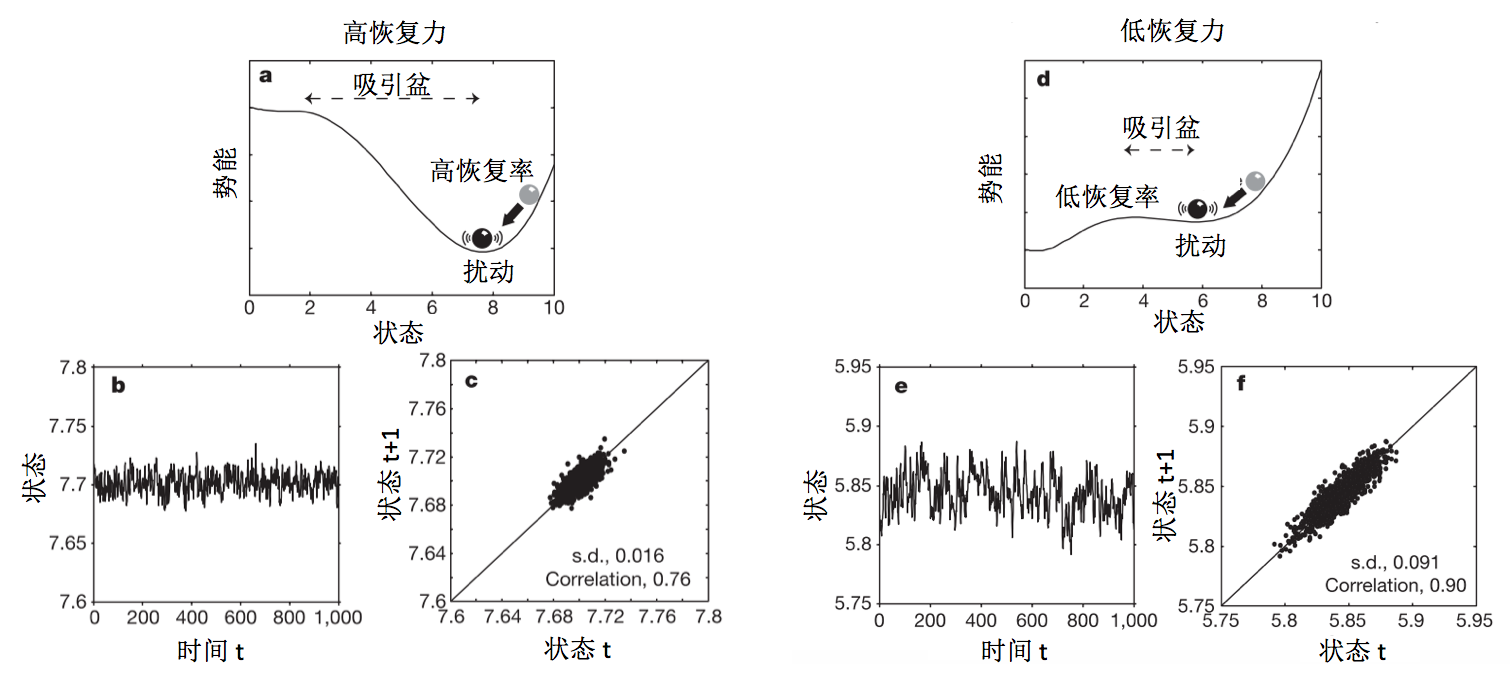
\includegraphics[scale=0.5]{figures/csd-early-warning-signal.png}
\caption{系统临近临界相变状态的特征示意图\cite{scheffer2009early}}
\label{fig:csd-early-warning-signal}
\end{figure}

临界相变点存在是动态系统固有的非线性和随机性导致的结果\cite{bar1997dynamics,endy2005foundations}。
一方面,以上针对预测临界相变点的早期预警特征均以系统的固有随机波动信号,即系统的随机不确定性,为基础。随机不确定性是随机动力学的显著特性\cite{scheffer2001catastrophic},并且“复杂系统理论适用于研究随机动力学系统的临界相变分析”这一论断已得到了大量研究证实\cite{van2007slow,longtin2010stochastic,carpenter2011early}。
另一方面,虽然工业系统似乎与生态系统有所不同,但类似于喷气发动机,机车和轴承这样的工程系统都属于动态系统,并且在复杂的内部因素和环境因素相互作用下表现出非线性行为和随机波动性\cite{strogatz2018nonlinear,cotilla2012predicting}。再者,工业系统的基础是物理学系统\cite{lee2015cyber},物理学系统由于受到外部干扰,例如温度、气候和人为操作等不确定性噪声的影响可增加系统的随机性,以及系统自身的计算复杂性和制造误差,使其普遍存在随机不确定性\cite{wolfram1985origins}。

综上所述,本文认为基于复杂系统随机不确定性分析预测临界相变点的理论可支持本文针对工业系统的失效分析,进而为工业系统的失效机理和普适性{\heiti 早期预警特征}学习提供新思路。再者,此过程只需依赖少量失效敏感时间序列进行学习,可有效应对故障数据小样本、不完备特性的挑战。

%中挖掘出来并且可以为预测潜在自然灾难提供解决方案\cite{scheffer2012anticipating}


% 结构特征
(2)复杂系统临界相变的结构特征

如图\ref{fig:csd-early-warning-structure},复杂系统的结构特征可分为两种,即复杂系统模块间的异构性和复杂系统模块间联系的同构性。其中异构性特征适用于各局部之间相关性不强的系统,而同构性特征适用于各局部之间存在强关联的系统。基于结构特征的改变可对系统临界相变进行预测。分析过程中,可将复杂系统抽象成由各局部构成的复杂网络,每个节点都存在多态性并且与相邻节点有着相互作用关系,比如生态系统中的共生关系、捕猎关系等。若系统中有局部节点发生状态变迁,这样的改变将会传递给相邻节点,以此递归极有可能产生大范围的级联反应,类似于多米诺骨牌效应,最终导致复杂系统整体结构产生变化。2016年,Gao 等人在《Nature》上发表的文章,基于生态系统物种间的关联关系构建相关性结构特征,对系统的变迁进行了很好的预测\cite{gao2016universal}。理论上来说这样的结构特征普遍存在于具有复杂耦合关系的系统中。
\begin{figure}[H]
\centering
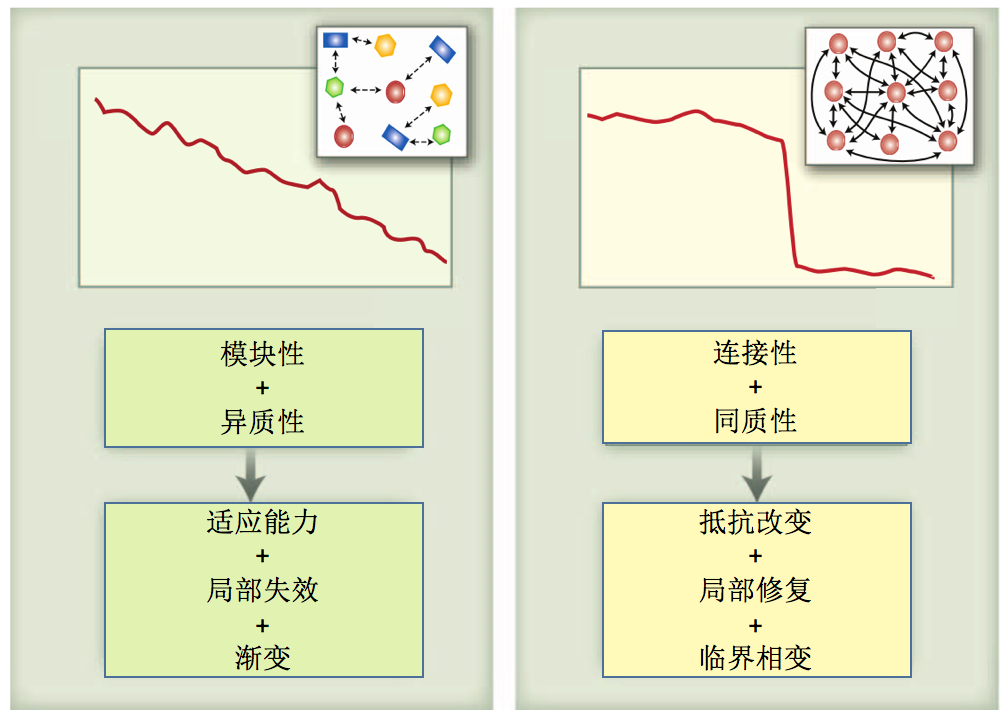
\includegraphics[scale=0.5]{figures/csd-early-warning-structure.png}
\caption{系统临近临界相变点的结构特征\cite{scheffer2012anticipating}}
\label{fig:csd-early-warning-structure}
\end{figure}

在工业系统中,各部件之间或多或少存在相互影响,如何从传感器采集的时序数据中构建相关性结构不变式已经得到广泛关注与研究。在2006年,Jiang 等人通过抽象时序数据之间的关联关系,构建了系统正常状态下的网络结构不变式,当系统局部失效时,结构不变性将会失效,基于此可预测系统异常或故障\cite{jiang2006discovering}。2015年,Han 等人通过构建复杂物理系统的相关性结构特征,对系统级的状态变迁进行了很好的识别\cite{han2015time}。

基于广泛调研与实际观察发现,复杂工业系统各局部的运行机制以及趋势往往存在较大差异,而其与自身历史以及与其他部件间的关联关系可以在给定状态下保持一致,或在可允许范围内轻微波动。综上所述,复杂系统结构特征可以作为{\heiti 高维多模态物理信号建模}的基础,进而有效的支持系统级的健康分析。

\section{生成式对抗网络}
\label{sec:gan-review}

% 深度学习的强大,但
神经网络在特征学习方面取得突破进展\cite{lecun2015deep},比如以绝对优势赢得2012年ImageNet图片分类比赛的深度卷积神经网络AlexNet\cite{krizhevsky2012imagenet}。其他对专家知识依赖很强的领域,比如生物\cite{webb2018deep}、医疗\cite{mirowski2008comparing}、工业\cite{tsui2015prognostics}等领域也纷纷引入神经网络探寻突破,其中,2008年,Mirowski 等人将卷积神经网络与传统机器学习方法逻辑斯蒂回归和支持向量机作比较,基于颅内脑电图扫描器采集的信号来预测癫痫发作,实验结果为:卷积神经网络的误报率最低,基于21个病例进行实验,只有一个误报,而SVM有10个误报\cite{mirowski2008comparing}。

% 大多为判别式模型。存在很多局限,难以进行广泛应用。
以上突破进展大多为基于判别式模型的监督式学习,需要大量标记数据作为训练集,然而获取高质量的标记数据仍是难题。对此,无监督式学习逐渐成为焦点\cite{lecun2015deep}。其中对数据底层分布进行学习的生成式模型是实现无监督式学习的主要方法,目前最主流的生成式模型有全可视信念网络(Fully Visible Belief Network, FVBN)\cite{frey1998graphical}、变分自编码机(Variational AutoEncoder, VAE)\cite{russakovsky2015imagenet}和生成式对抗网络(GAN)\cite{goodfellow2014generative}。GAN 因具有以下优势而倍受青睐:(a) 计算高效:GAN 可以并行生成样本,相比之下FVBN只能串行生成样本效率很低;GAN的训练过程基于快速的反向传播和梯度下降方法,不需要进行马尔可夫链蒙特卡洛(Markov Chain Monte Carlo, MCMC)估计和统计推理(Inference)等耗时的运算,相比之下玻尔兹曼机对MCMC的依赖正面临着计算困难的问题\cite{salakhutdinov2010efficient}。(b) 统计优势:GAN 由生成器和判别器组成,其中生成器负责学习数据的分布,其训练优化由判别器驱动,避免了直接复 制数据的风险,即对过拟合具有天然的抵抗能力。(c)可以学习复杂分布:GAN 由基于神经网络的复杂函数构成,可以学习非常复杂的分布。(d)局限性少:GAN不需要像VAE那样设计变分约束,其基本框架已保证训练过程的全局收敛性;GAN 对生成函数的限制很少,相比之下玻尔兹曼机需要精心设计MCMC过程存在诸多局限。(e)大量实践表明,相比其他主流生成式模型所生成的样本,GAN 生成样本的质量更高。当然GAN也有不足,主要表现为以下两个方面:(a)GAN 的生成器可用于数据生成,但没有显示的表达式。(b)训练过程不稳定,判别器的更新必须要与生成器同步,否则会导致模式崩溃(Mode Collapses),即生成器所表示的分布只能收敛于真实数据集分布的少量模式,缺乏多样性。

GAN 为无监督式学习开辟了新道路,已得到广泛研究和应用,随着不断发展其劣势已逐步得到攻克\cite{radford2015unsupervised},然而鲜有针对时间序列数据的成果,因此本文基于GAN研究{\heiti 通用的无监督式时间序列特征学习}方法具有重要意义。

% 以上优势是我自己根据 tutorial 和 primitive paper 进行总结的结果。

% 来自goodfellow的tutorial
% (1)GAN 可以并行的生成样本,相比于FVBN串行生成样本的方式更高效;(2)GAN 的生成函数限制很少,相比于对马尔可夫过程具有强依赖的玻尔兹曼机(Boltzmann machines)\cite{salakhutdinov2010efficient}更灵活;(3)GAN 的运算不需要类似于玻尔兹曼机运算时的马尔可夫过程,因此更快更高效;(4)GAN不需要像VAE那样设计变分约束,其基本框架已保证训练过程的全局收敛性;(5)大量实践表明,相比于主流生成式模型所生成的样本,GAN 生成样本的质量更高。

% 无监督式学习旨在基于更容易获取的无标记数据学习具有强泛化能力的模型,限制性玻耳兹曼机(Restricted Boltzmann Machine)\cite{salakhutdinov2010efficient}、自动编码机(Auto-Encoder)\cite{vincent2008extracting}和概率图模型(Probability Graph Model)\cite{lee2009convolutional}等都是实现无监督式学习的重要模型,并且大多为学习数据隐含分布的生成式模型。另外,2014 年 Ian J. Goodfellow 等人创造性的提出生成式对抗网络为无监督式学习开辟了新道路\cite{goodfellow2014generative}。
% 【LeCun认为这是近10年来神经网络领域最重要的突破。】

% 介绍 GAN 的定义
(1)生成式对抗网络简介

图\ref{fig:gan-gan}(左)为生成式对抗网络(GAN)的基本结构,其核心由两个神经网络构成,即生成器(Generator, G)和判别器(Discriminator,D)。生成器负责学习数据的分布,基于输入的噪音 \emph{z} 生成逼真的假样本\emph{X'};判别器负责判断输入数据的真假,从输入数据中识别真实样本\emph{X}。GAN的训练过程是生成器和判别器两者间的博弈,生成器基于判别器的反馈不断优化以生成尽可能逼真的样本为目标;与此同时判别器不断提高自身的判别能力来辨别越来越逼真的假样本。原文以造假币的罪犯(生成器)和警察(判别器)之间的博弈作为类比,造假币的罪犯不断提高自身技能以生成逼真的假币为目标,同时警察不断提升自身侦查力以准确地判别钱币真伪为目标。这样的博弈一值持续直到警察(判别器)无法辨别钱币(样本)真伪为止。假设有服从分布$P_{data}$的真实数据集和服从分布$P_{z}$的噪音\emph{z}作为模型输入,GAN的基本结构和训练过程具体的定义如下:
\begin{figure}[H]
\centering
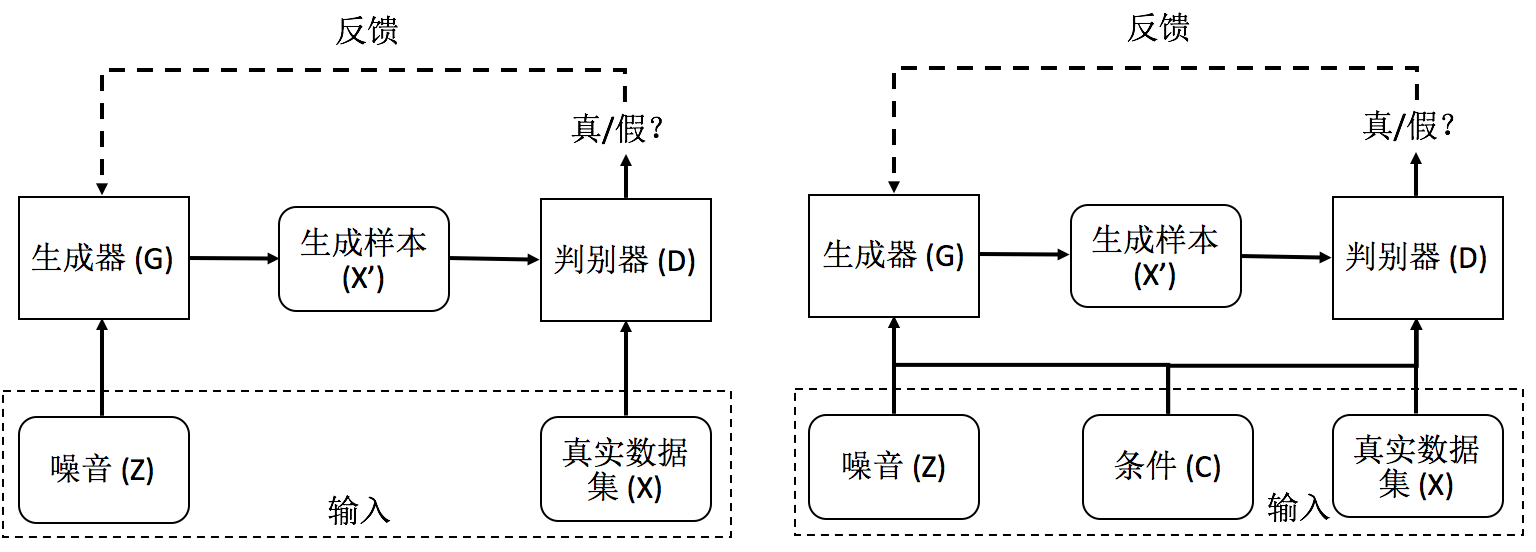
\includegraphics[scale=0.5]{gan-gan.png}
\caption{(左)生成式对抗网络,(右)条件生成式对抗网络}
\label{fig:gan-gan}
\end{figure}

1. 生成器:生成器是以$\theta_{g}$为参数的可导函数,以噪音\emph{z}为先验,通过映射$G(z;\theta_{g})$来学习真实数据分布$P_{data}$,即$G(z;\theta_{g})$实现噪音\emph{z}到样本$x$的映射,并且$G(z;\theta_{g})$可看作分布$P_{g}$表示对$P_{data}$的近似估计。

2. 判别器:判别器是以$\theta_{d}$为参数的可导函数$D(x;\theta_{d})$,对输入样本$x$的真假进行判别(真表示样本$x$来自$P_{data}$,否则表示样本来自$P_{g}$)。判别器实际上是监督式学习中的二分类器,判别器的输出$D(x)$为[0,1]区间上的实数,表示输入样本$x$为真的概率,即表示样本\emph{x}来自$P_{data}$而非$P_{g}$的概率。

3. GAN的训练:GAN的训练过程是由等式\ref{eq:gan-objective-function}定义的最大最小化博弈,该函数基于分类器交叉熵函数来定义,以此为目标函数判别器和生成器通过随机梯度下降和反向传播优化方法进行迭代更新。一方面判别器作为二分类器,以准确判别样本真伪为目标,即最大化真样本的概率并最小化假样本的概率,对应等式\ref{eq:gan-objective-function}的内层最大化过程;另一方面生成器需要基于判别器的反馈进行更新,对应等式\ref{eq:gan-objective-function}外层的最小化过程,即最小化$log(1-D(G(z)))$。等式\ref{eq:gan-objective-function}有全局最优解$P_{g}=P_{data}$,此时判别器无法分辨样本真伪也就不会再产生误差进而训练过程因达到纳什均衡而停止。理论上只要给予GAN足够的能力和训练时间就可达到纳什均衡,具体证明可参考原文\cite{goodfellow2014generative}。
\begin{equation}
\label{eq:gan-objective-function}
  \min_{G}\max_{D} V(D,G) = \mathbb{E}_{x \sim P_{data}(\bf{x})}[log(D(x))] + \mathbb{E}_{z \sim P_{z}(\bf{z})}[log(1-D(G(z)))]
\end{equation}

目标函数\ref{eq:gan-objective-function}便于理论分析,但在实际应用中不总是能产生足够的梯度来优化生成器。在训练初期,生成器的能力很弱,因此其生成的样本质量很差,这样一来判别器很容易辨识生成器生成的假样本,即$D(G(z))$很小,小到接近于0,进而导致$log(1-D(G(z)))$逼近0,以至于梯度消失,此时判别器对生成器只能产生近乎可忽略的微小反馈。因此在实际应用中,对生成器的训练不直接最小化$log(1-D(G(z)))$而是启发性的以最大化$log(D(G(z))$为目标,这样的修改不会影响模型的收敛性并且可以保证生成器在训练初期可得到更大的梯度进行迭代更新。

% % review 当前 GAN 的发展情况
(2)生成式对抗网络研究现状

1. 在结构改进方面

针对GAN训练不稳定的问题,2014年,Mirza 等人提出条件生成式对抗网络(Conditional GAN, CGAN)学习数据的条件概率分布\cite{mirza2014conditional},如图\ref{fig:gan-gan}(右),基于原始GAN加入条件先验(比如样本标记)以限制GAN的训练过程使其不再那么天马行空。在有先验的情况下GAN可以很直接的扩展为CGAN,因此GAN和CGAN通常成对出现。
%值得注意的是,给定的先验条件可以是除样本标记以外的假设或约束。
2015年,Denton 等人基于拉普拉斯算子的金字塔(LAplacian Pyramid)框架融合多个GAN以实现图片数据生成,模型简称为LAPGAN\cite{denton2015deep}。LAPGAN通过若干个基于卷积神经网络的GAN生成多个不同像素的图片,然后融合以上输出结果得到最终的生成样本图片。
2015年,Radford 等人提出深度卷积生成式对抗网络(Deep Convolutional GAN, DCGAN)\cite{radford2015unsupervised},使生成样本的质量有了质的飞跃,此后的大多成果都基于DCGAN进行改进。值得注意的是,虽然LAPGAN也使用卷积神经网络作为基础,但与LAPGAN级联融合不同的是DCGAN改进了生成器中卷积神经网络的基本操作,第一次实现单次生成高分辨率图片。DCGAN几个核心的改进为(a)将判别器的池化层替换为跨步卷积(Strided Convolutions),将生成器的池化层替换为小数跨步卷积(Fractional-Strided Convolutions);(b)生成器和判别器都使用批规范化(Batch Normalization);(c)去掉传统深度神经网络中的全连接隐藏层;(d)对生成器的激活函数作如下设置:除了输出层使用Tanh激活函数以外所有单元都使用ReLU作为激活函数;(e)判别器的所有单元都使用LeakyReLU作为激活函数。

2. 在理论改进方面

有部分研究聚焦于GAN的目标函数和训练方式,尝试对GAN的基础理论进行改进。2016年,Chen 等人提出InfoGAN(Information GAN)实现了完全无监督式学习\cite{chen2016infogan},基于信息论改进GAN的目标函数,通过最大化固定大小的噪音子集和观察样本之间的互信息来鼓励GAN学习可解释且有意义的特征。2017年,Arjovsky 等人提出WGAN(Wasserstein GAN)\cite{arjovsky2017wasserstein},从理论上对GAN的核心困难作出重大改进,主要贡献有:(a)解决了GAN训练不稳定问题;(b)设计瓦瑟斯坦距离(Wasserstein Distances) 作为优化新指标。

3. 在应用探索方面

基于GAN的应用已取得很多重要突破,比如基于GAN实现图片翻译\cite{isola2017image} 、基于GAN实现图片分辨率提升\cite{ledig2016photo} 、基于GAN实现文本到图片的翻译\cite{reed2016generative} 。另外,2016年,Salimans 等人针对GAN的训练问题提出了多种启发式的改进\cite{salimans2016improved},所涉及的方法有特征匹配(Feature matching)、小批量辨识(Minibatch discrimination)、单边标记平滑(One-sided label smoothing)和虚拟批规范化(Virtual batch normalization)。

综上所述,GAN已得到广泛应用和验证。然而现有突破大多局限于计算机视觉和自然语言处理领域,鲜有针对时间序列数据的研究。2018年,Creswell等人为信号处理领域作了有关GAN的研究综述,但鲜有针对时间序列数据的成果\cite{creswell2018generative}。本文至今只关注到医疗领域有相关初探性研究\cite{esteban2017real,yahi2017generative,choi2017generating},然而他们提出的模型都只在一个医疗时间序列数据集上进行验证,不具备普遍适用性。
% !TEX root = ../main.tex

\chapter{基于符号回归的系统结构特征学习与应用}
\label{chap:symbolic-regression}

\section{引言}
\label{sec:sr-intro}

铁路运输具有规模大、经济、节能等优势使其在人类社会中扮演着重要角色\cite{2015年交通运输行业发展统计公报}。高速列车是典型的工业系统,本章主要针对以轴温为代表的设备正常状态数据——高速列车轴承温度正常状态数据,开展数据驱动的机理挖掘研究。
%以中国铁路运输为例,支持中国25\%的运输量,能源消耗仅占所有运输方式总消耗的6\%\cite{2015年交通运输行业发展统计公报}

% PHM 技术在实际应用中的局限。
故障预测是 PHM 的核心要义,基于模型的故障预测方法,机理知识清晰、预测精度高,然而局限于系统机理透明并且对精度要求很高的领域;
数据驱动的故障预测方法,具有良好的灵活性便于实际应用,然而现有方法大多针对任务直接建模,缺乏对系统机理的认识\cite{lee2014prognostics,彭宇2010故障预测与健康管理技术综述}。再者,PHM 技术在机车系统中的应用仍存在诸多挑战:(a)现代机车已演变成高度复杂的工程机械,其正常运行需要依赖多个学科的统一,涉及力学、热力学、机电、电子、计算机和控制工程;(b)不同的运输目标和环境要求机车模型必须具备多样化特性,实际上机车服务年限已长达30年,系统化的PHM方案必须能应对多种机车组的不同需求;(c)制造业的全球化进程和复杂的设备所有权关系使建立全面的知识库面临巨大困难。
%(1)现代机车已演变成高度复杂的工程机械,其正常运行需要依赖多个物理学科的统一,涉及力学( Mechanics)、热力学(Thermodynamics)、机电(Electromechanics)、电子(Electronics)、计算机(Computers)和控制工程(Control engineering)。

一方面,本文通过实际调研发现,来自不同传感器和/或不同车轴的信号存在强相关性。如图\ref{fig:csd-early-warning-structure},复杂系统的结构特征分为两种,其中同构性特征适用于各局部之间存在强关联的系统\cite{jiang2006discovering,han2015time}。另一方面,符号回归系统辨识方法已受到广泛关注\cite{schmidt2009distilling,la2016automatic,mcconaghy2011ffx,fortin2012deap},具有纯数据驱动、对非线性系统的抽象能力、可同时实现结构选择和参数学习等诸多优势,并且其所学系统方程具备良好的系统结构表达能力。

综上所述,本章首先提出基于符号回归的系统结构特征学习方法,并融合确定性优化算法和遗传算法完成训练,由此揭示系统的底层物理机理。然后将所学系统结构特征作为健康基线,设计在线实时异常检测框架。
  
%We prove that modern data mining techniques are able to identify the internal dynamics of bearing through the temperature data and perform accurate prediction.

%In this work, we develop a hot-axle prediction and analysis framework. The framework is deployed in the locomotive monitoring data center to perform online fault prediction and diagnosis. It takes the multivariate sensor time series as input. The details of sensor data are listed in Table 1

%Different from existing data driven PHM studies, which typically use experimental data to extract patterns for anomaly detection/prediction under the guidance of domain knowledge, our framework performs online and off-line fault prediction by exploiting sensor data collected during regular operations. We prove that modern data mining techniques are able to identify the internal dynamics of bearing through the temperature data and perform accurate prediction

\section{数据采集}

%axle:轮轴(车轴),bearing:轴承

(1)数据采集装置

% 并且近年来已有研究工作关注热轮轴温度的预测问题\cite{ma2016prediction,yi2015faults,amini2016wayside},在一定程度上说明温度数据对系统性能的敏感性
% “中国机车远程监测与诊断系统”
如图\ref{fig:sr-data-collect}是机车和数据采集环境。实际工程中温度传感器已得到广泛部署,温度数据最为丰富。一辆机车有6个轮轴,每个轮轴配置8个传感器,这些传感器都统一配置为温度传感器。每个轮轴的8个传感器被部署于不同位置,其中2个分别放置于轮轴两端以感知环境温度,剩下的6个传感器均匀的分配到轮轴的2个轴承上。每个轴承有3个传感器,分别部署在轴承的左上方、上方和右上方。除了关键的轴承温度外,本文还采集了火车管道压力、停车制动压力、平衡油缸压力、火车管流和机车运行速度数据,具体的数据说明见表\ref{tab:sr-variables}。

\begin{figure}[H]
\centering
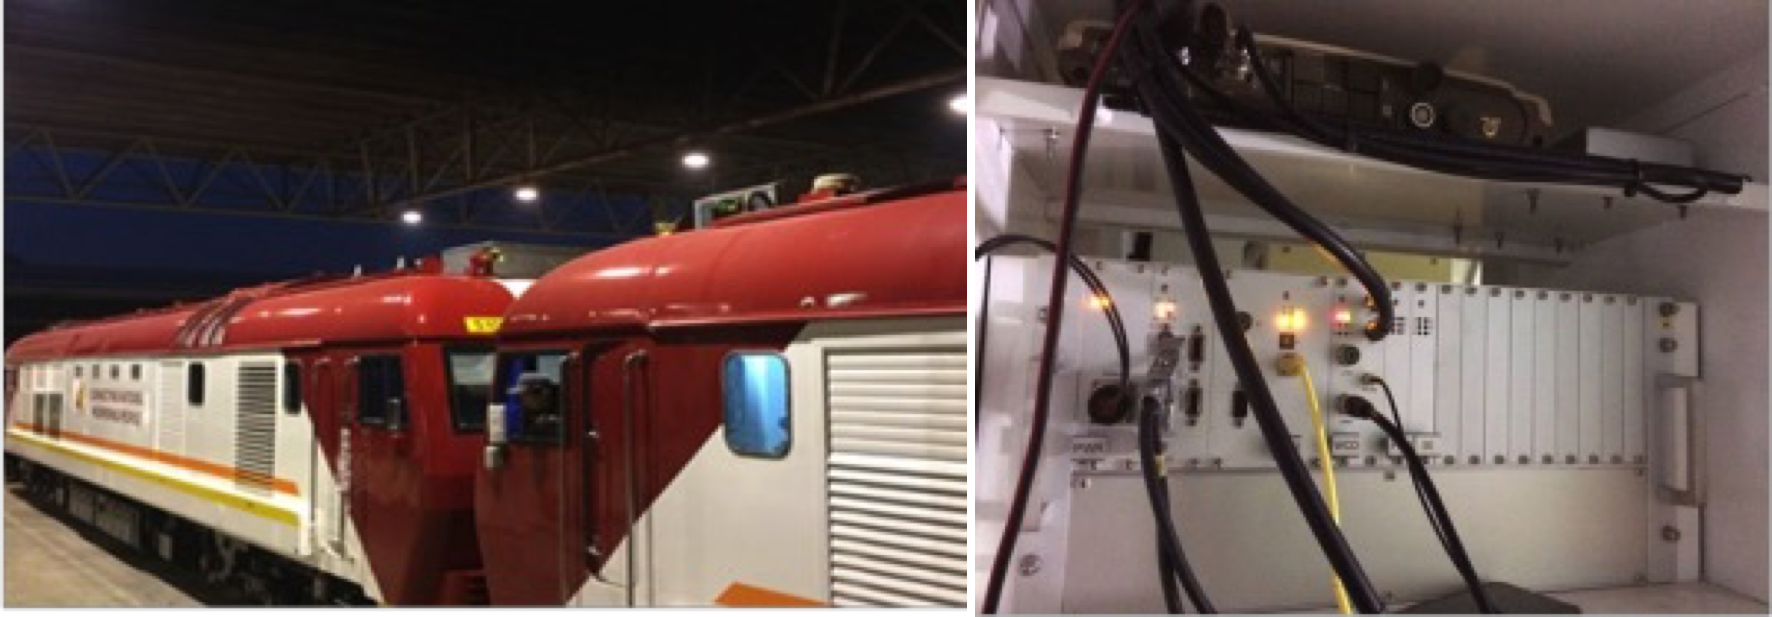
\includegraphics[scale=0.5]{figures/sr-data-collect.png}
\caption{机车和数据采集设备}
\label{fig:sr-data-collect}
\end{figure}

\begin{table}[htbp]
  \centering
  \caption{高速列车走行部的多元时间序列数据}
  \label{tab:sr-variables}
  \begin{tabular}{cc}
    \toprule
    {\heiti 变量名} & {\heiti 描述} \\\midrule[1pt]
    ZD\_LCG & 火车管道压力 \\
      ZD\_TFG & 停车制动压力 \\
      ZD\_JHG & 平衡油缸压力 \\
      ZD\_LLJ & 火车管流 \\
      ZD\_SPEED & 机车运行速度 \\
      ZD\_HW\_N\_1 & 轴承 N 左边的环境温度 \\
      ZD\_HW\_N\_2 & 轴承 N 右边的环境温度 \\
      ZD\_WD\_N\_Y & 轴承 N 在位置 Y 的温度 
    \\\bottomrule
  \end{tabular}\\[1.5pt]
\end{table}

(2)数据分析

1. 数据预处理

本文数据预处理主要由三部分组成。(a)数据集成:汇总不同维度的传感器数据并进行时间对标以保证数据的一致性。(b)数据清洗:本文首先基于少量先验知识去掉明显冗余的数据。针对传感器在数据采集过程中由于受到复杂环境的影响,存在数据丢失和噪音的情况,本文通过平滑处理方法消除干扰噪音(比如去除固定幅度和时间间隔的周期性波动噪音)。(c)重采样:实际采样频率因复杂环境因素不同而不同、再者数据存在缺失和噪音,无法满足符号回归方法中时间序列等间隔采样的前提假设
。对此本文采用适当的重采样技术对传感器时间序列进行预处理以保证各采样点之间保持相等的时间间隔\cite{good2006resampling},通过多次实验验证发现高斯插值对数据处理的效果最好。
\begin{figure}[H]
\centering
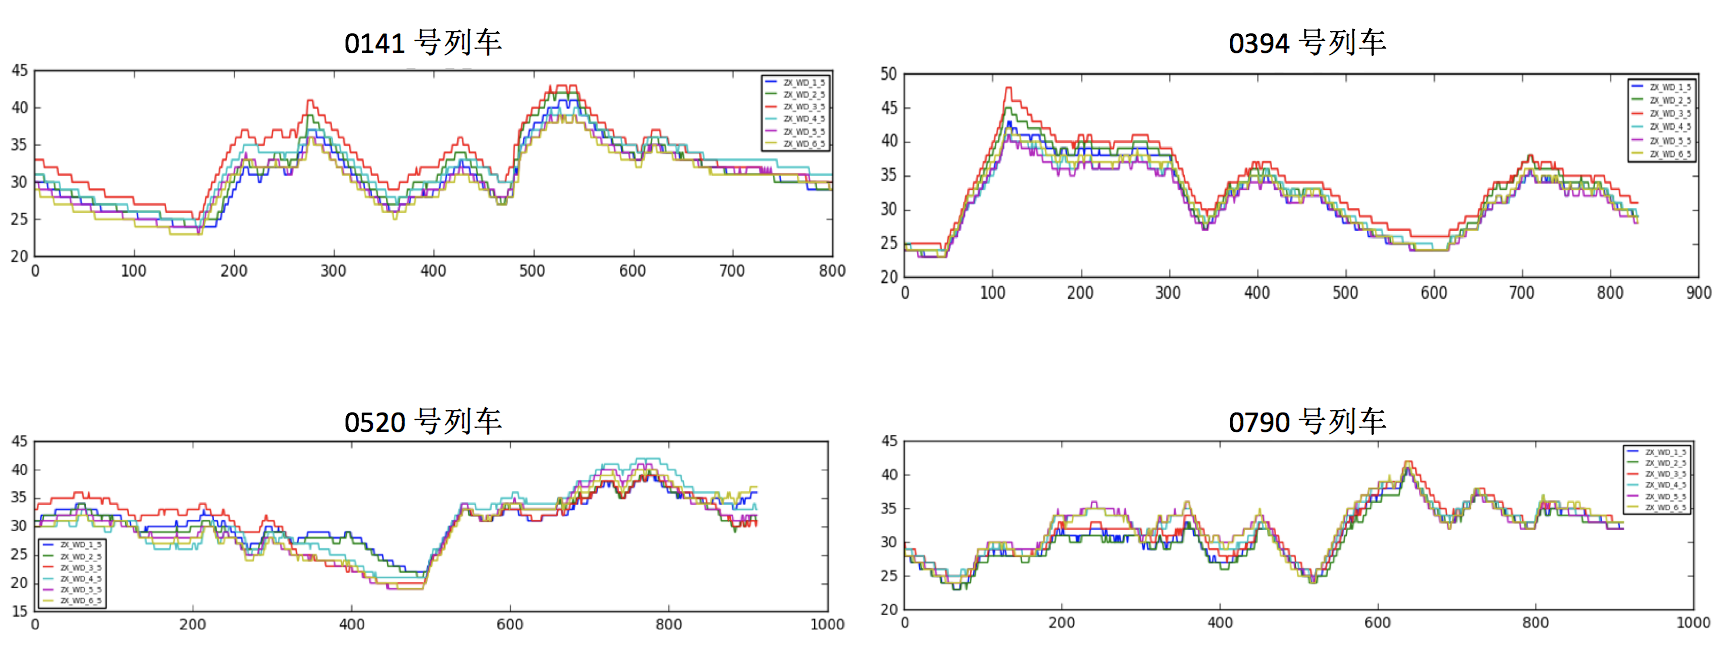
\includegraphics[scale=0.5]{figures/sr-data-temp.png}
\caption{不同高速列车不同观测点的温度数据}
\label{fig:sr-data-temp-corr}
\end{figure}  

2. 数据探索

本文对若干机车组三个月的温度数据进行探索,利用多种可视化方法或工具对数据进行理解、通过先进的时间序列分析方法检查温度数据的稳定性和相关性,具体方法细节参考Bisgaard 等人的著作\cite{bisgaard2011time}。主要有以下发现:
\begin{itemize}
  \item 温度数据的采样率在1/10Hz到10Hz之间。
  \item 环境和车轴温度具有时变和不稳定的性质。事实上,轴承的内部动态性会根据不同的工作模式而改变。
  \item 轴承内部温度由\ref{eq:data-temp-generate}解析式决定\cite{陈德生2003列车轴温规律及红外线轴温探测方式的研究}。车轴的最大稳定温度为$t_{stable}$,由以下几个因素决定,车轴直径和车轮直径的比值 $(\frac{D_{axle}}{D_{wheel}})$,车轴盒压力 (\emph{P}),机车速度 (\emph{V}),摩擦因子(\emph{f}),和散热能力$(\sum {\alpha_{i}F_{i}})$的倒数。车轴盒表面的温度上升速度为\emph{m},由散热能力$(\sum {\alpha_{i}F_{i}})$和热吸收能力$\sum {C_{i}P_{i}}$的比值决定。$t_{raise}$表示温度上升遵循指数方程。
  \item 轴承内部状态通常无法直接探测。不同位置感知的温度数据由影响轴承状态的多种因素决定,包括但不仅限于机车的工作状态(比如,运行速度和牵引水平),传感器和轴承的相对位置,环境因素(比如环境温度和路线特点),以及其他多种外部干扰因素(比如空调系统的散热)。总的来说,来自不同传感器和/或不同车轴的数据存在强相关性但相关的模式会因工作状态的改变而变化。如图\ref{fig:sr-data-temp-corr}所示,不同列车的车轴温度数据形状各异,但不同轴位点之间的温度数据存在强相关性。
  \item 传感器数据存在高噪的特性。传感器工作过程中会受到多个噪音源的影响,比如来自车载空调系统的排气口的影响。
  \item 轴承失效模式具有高度复杂性。在当前的机车上,当传感器测量值超过预设阈值时车载监控系统将产生失效报告。然而,这样基于域值的方案无法用于预防性维修。此外,一个固定的域值无法覆盖所有失效模式。事实上,温度梯度的上升和多种温度亚域值峰值可以反应系统失效。
\end{itemize}
\begin{equation}
\label{eq:data-temp-generate}
\left\{\begin{array}{l}
t_{stable} = \frac{D_{axle}\ast P\ast f \ast V}{D_{wheel}\ast \sum \alpha_{i}F_{i}}  \\[0.2cm]
t_{raise} = t_{stable}\ast (1-e^{-m\tau}) \\[0.2cm]
t_{sink} = t_{stable} \ast e^{-m\tau} \\[0.2cm]
m = \frac{\sum \alpha_{i}f_{i}}{\sum C_{i}P_{i}}
\end{array}\right.
\end{equation}

\section{系统结构特征学习}
\label{sec:sr-feature}

(1)符号和变量定义

\begin{itemize}

  \item 令小写字母黑体表示向量,即$\mathbf{a,b,c,d,...,x,y,z}$。

  \item 令大写字母黑体表示矩阵,即$\mathbf{A,B,C,D,...,X,Y,Z}$。

  \item 假设数据采样点为$\mathbf{t}=[t_{1},t_{2},...,t_{n}]$,以时间为单位非递减有序,默认等间隔。

  \item 假设一次采样结果为$(\mathbf{X},\mathbf{y})$,其中$\mathbf{X}$为{\heiti 因变量},$\mathbf{y}$为{\heiti 目标变量}。
  因变量$ \mathbf{X} \in R^{n\times m} $定义为\ref{equ:sr-object-func-x},是\emph{n}行和\emph{m}列矩阵,\emph{n}行表示对应$\mathbf{t}$的\emph{n}个时刻的观测结果,\emph{m}列表示\emph{m}个不同观测变量。
  目标变量$\mathbf{y}$定义为\ref{equ:sr-object-func-y},是对应$\mathbf{t}$的\emph{n}个时刻的观测结果。

  \item 假设有{\heiti 运算子}集合$\mathbf{P}$,定义如\ref{equ:sr-ops},其中每个元素表示一个基本的算数运算。当前运算包括:
  加法运算$add(\mathbf{x,y})$表示两个输入向量的和,即返回$\mathbf{x}+\mathbf{y}$;
  减法运算$sub(\mathbf{x,y})$,表示两个输入向量的差,即返回$\mathbf{x}-\mathbf{y}$;
  乘法运算$mul(\mathbf{x,y})$,表示两个输入向量的点积,即返回$\mathbf{x} * \mathbf{y}$;
  除法运算$divide(\mathbf{x,y})$,表示两个输入向量的商,即返回$\mathbf{x}/\mathbf{y}$;
  正弦运算$sin(\mathbf{x})$,返回输入向量的正弦运算结果;
  余弦运算$cos(\mathbf{x})$,返回输入向量余弦运算结果;
  对数运算$log(\mathbf{x}, i) $,返回输入向量的对数运算结果,即返回$log_{i}(\mathbf{x})$;
  幂运算$pow(\mathbf{x}, i)$,返回输入向量的幂运算结果,即返回$\mathbf{x}^{i}$;
  取最大值运算$max(\mathbf{x})$,返回输入向量的最大值;
  取最小值运算$min(\mathbf{x})$,返回输入向量的最小值。
  \item 基函数向量$\mathbf{\Psi}$,定义如\ref{equ:sr-basefunc},一共有$n_{b}$个元素,其中每个元素$\varphi_{i}$表示一个{\heiti 基函数},基函数是由运算子集合$\mathbf{P}$中若干个运算子构成的线性或非线性复杂函数。

\end{itemize}
\begin{subequations}
\begin{align}
\mathbf{X} &= \begin{bmatrix}
x_{1}(t_{1}) & x_{2}(t_{1}) & ... & x_{m}(t_{1}) \\ 
x_{1}(t_{2}) & x_{2}(t_{2})  & ...  & x_{m}(t_{2}) \\ 
... & ... & ...  & ... \\ 
x_{1}(t_{n}) & x_{2}(t_{n})  & ...  & x_{m}(t_{n}) 
\end{bmatrix} = [x_{1}(\mathbf{t}), x_{2}(\mathbf{t}), ..., x_{m}(\mathbf{t})] = [\mathbf{x_{1}}, \mathbf{x_{2}}, ..., \mathbf{x_{m}}] \label{equ:sr-object-func-x} \\
\mathbf{y} &= [y(t_{1}), y(t_{2}), ..., y(t_{n})]^{T} \label{equ:sr-object-func-y}\\
\mathbf{P} &= \begin{bmatrix}
add(\mathbf{x,y}) & sub(\mathbf{x,y}) & mul(\mathbf{x,y}) & divide(\mathbf{x,y}) \\ 
sin(\mathbf{x}) & cos(\mathbf{x}) & log(\mathbf{x}, i) & pow(\mathbf{x}, i) \\ 
max(\mathbf{x})& min(\mathbf{x}) & ... & ...  \\ 
\end{bmatrix} \label{equ:sr-ops} \\
\mathbf{\Psi} &= [\varphi_{1}, \varphi_{2}, ..., \varphi_{n_{b}}] \label{equ:sr-basefunc} 
\end{align}
\end{subequations}

(2)基于符号回归的系统结构特征学习的框架

\begin{figure}[H]
\centering
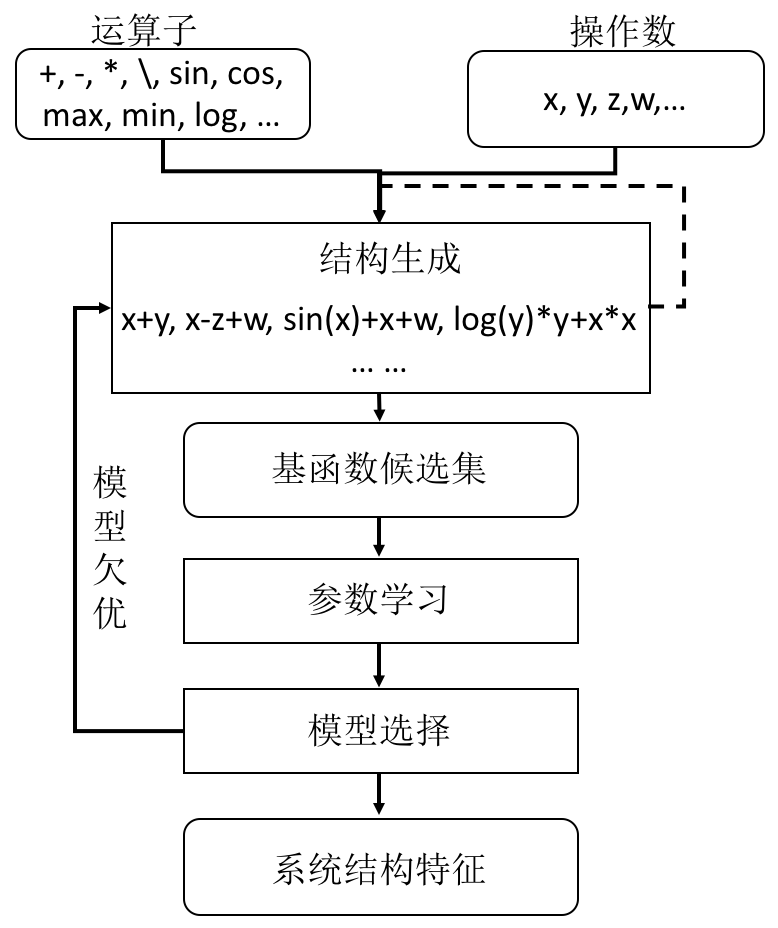
\includegraphics[scale=0.5]{figures/sr-anomaly-framework-feature.png}
\caption{基于符号回归的系统结构特征学习框架}
\label{fig:sr-feature}
\end{figure}

图\ref{fig:sr-feature}是基于符号回归的系统结构特征学习框架,具体流程如下:
\begin{enumerate}[1.]
  \item 初始化:设定运算子集合$\mathbf{P}$,定义为\ref{equ:sr-ops},作为基函数集合$\mathbf{\Psi}$的初始值。输入因变量$\mathbf{X}$作为操作数,以及对应的目标变量$\mathbf{y}$作为评估指标计算的参考。
  \item 结构生成:从基函数集$\mathbf{\Psi}$优选若干个基函数作为运算子或操作数组合形成新的更复杂的基函数,并将其加入到当前基函数集合中。由此循环迭代,通过结构评价指标控制基函数集的大小和质量,当迭代触发域值时停止,并将基函数集合输入到下一环节。
  \item 参数学习:对输入的基函数集$\mathbf{\Psi}$进行融合,即通过回归模型\ref{equ:sr-object-func}对目标变量进行估计,通过计算估计量$\mathbf{\hat{y}}$和实际观测量$\mathbf{y}$的误差来进行模型参数学习。即对模型\ref{equ:sr-object-func}的参数$\{a_{i}\},i=1,...,n_{b}$和$\mathbf{b}$进行学习。
  \item 模型选择:通过模型评价指标对模型$f(\mathbf{X})$的质量进行评价,从而作出是否接受当前学习结果的决策,若对学习结果不满意则返回第2步,甚至可以返回第1步对模型输入进行调整。若对学习结果满意,则将当前模型输出。
  \item 结束:最后框架的输出为一个或若干个优选的模型,定义为\ref{equ:sr-models},并给出各模型的评价。这些模型可以表达系统的底层动态特性和运行机理,还可以为后期其他任务提供支持。
\end{enumerate}
\begin{subequations}
\begin{align}
\mathbf{\hat{y}} &= f(\mathbf{X}) = \mathbf{b} + \sum_{i=1}^{n_{b}}a_{i} \ast \mathbf{\Psi}_{i}(\mathbf{X}) =  \mathbf{b} + \sum_{i=1}^{n_{b}}a_{i} \ast \mathbf{\Psi}_{i}(\mathbf{\mathbf{x_{1}}, \mathbf{x_{2}}, ..., \mathbf{x_{m}}}) \label{equ:sr-object-func} \\
\mathbf{M} &= [f_{1}, f_{2}, ..., f_{n_m}] \label{equ:sr-models} 
\end{align}
\end{subequations}

(3)基于符号回归的系统结构特征学习的训练优化算法

本文融合 FFX\cite{mcconaghy2011ffx} 和 Deap\cite{fortin2012deap}作为框架中结构生成以及参数学习引擎。前者用于生成初始解,而后者则用于对FFX产生的结果进行修剪以形成更简化的模型。核心思想如下:

首先执行 FFX 算法获取初始解,有以下 3 步:
\begin{enumerate}[1.]
      \item 通过确定性的方式产生一个大规模的基函数集。
      \item 识别最优的基函数并使用路径规整学习进行参数学习。
      \item 通过最小化错误率和复杂度的目标过滤掉冗余候选函数。
\end{enumerate}

将 FFX 输出的最优模型集进行解析,由此得到基函数集作为Deap 遗传编程的初始输入,然后循环执行以下3个步骤,直到收敛为止:
\begin{enumerate}[1.]
      \item 繁殖步:基于当前候选集产生新的候选集(即子孙)并通过突变和交叉操作保证种群的多样性。
      \item 评估步:对上一步产生的子孙进行评估。
      \item 选择步:基于上一步的评估结果选择优秀的子孙构成下一代的种群。
\end{enumerate}

(4)基于符号回归的系统结构特征学习的评价指标

1. 参数学习模块:以最小化误差平方和为优化目标,即最小化等式\ref{equ:sr-loss-rmse}。

2. 模型选择模块,不同于一般的回归方法,本文同时考虑模型准确率和模型可解释性,分别由准确率因子和理解性因子度量。准确率因子为估计值和真实值的误差平方和,定义为等式\ref{equ:sr-loss-rmse}。理解性因子由模型规模度量,定义为\ref{equ:sr-loss-complexity},由基函数个数表示,基函数越多说明函数越复杂进而表明可解释性越差。综上可得最终的模型选择度量指标\ref{equ:sr-loss},其中参数$\lambda$用于平衡两个因素的重要程度。
\begin{subequations}
\begin{align}
L &= RMSE + \lambda C \label{equ:sr-loss} , \lambda \in [0,1]\\
RMSE &= \sqrt{\frac{\sum_{i=1}^{n} (\hat{y_{t_{i}}} - y_{t_{i}})^{2}}{n} } \label{equ:sr-loss-rmse} \\
C &= size(f(\mathbf{X})) \label{equ:sr-loss-complexity}
\end{align}
\end{subequations}

\section{系统结构特征应用}
\label{sec:sr-application}

一方面,系统结构特征揭示了多信号间的相互作用关系,可直接支持用户理解系统的运行机理;另一方面,系统结构特征是系统状态的直接反映,通过正常运行数据学习的结构表达式可作为系统的健康基线,支持在线实时异常检测。再者,值得一提的是系统结构特征还支持了本文第\ref{chap:critical-transection}章的动态系统稳定性分析。

在当前的机车上,温度上升遵循指数方程是异常检测的主要依据,当传感器测量值超过预设阈值时车载监控系统将产生失效报告。然而轴承失效模式具有高度复杂性,基于固定阈值的异常检测难以具备复杂环境的自适应能力。由此,本文将通过正常运行数据离线学习的结构表达式作为系统运行的健康基线,设计在线实时异常检测框架,如图\ref{fig:sr-application},主要有以下内容:

(1) 数据采集

列车运行过程产生的数据主要通过传感器进行采集。有两个主要的数据流向,一方面,采集的数据将会被传输到数据中心的数据库中进行有效存储;另一方面,实时感知数据将会作为在线实时异常检测的输入。

(2) 在线实时异常检测
\begin{enumerate}[1.]
    \item 获取系统结构模型的生成数据作为健康基线:通过基于符号回归的系统结构特征学习框架提供的最优系统结构模型$f_{best}$,即通过等式\ref{equ:sr-predict},估计最近$w$个时刻内的信号轨迹$\mathbf{\hat{y}}$作为健康基线。
    \item 获取实时感知数据:通过传感器获取最近$w$个时刻内的实时监测数据$\mathbf{y}$。
    \item 残差生成:$\mathbf{\hat{y}}$和$\mathbf{y}$被同时输送到残差生成器,残差生成器通过等式\ref{equ:sr-residual}计算系统实时偏差。
    \item 误差估计:本文采用平均误差,定义为\ref{equ:sr-metrics},主要基于以下考虑:(a)由轴承内部温度解析式\ref{eq:data-temp-generate}可知,系统失效时轴承温度升高$t_{raise}$遵循指数方程,平均误差足以发现异常;(b)整个在线异常检测框架需要满足实时计算,实际项目仍难以支持过于复杂的评估方法,可待将来进一步优化。
    \item 异常决策:基于误差估计的结果,通过等式\ref{equ:sr-loss-alarm}作出是否报警的决策,其中$\alpha$为报警域值,根据实际应用需求而定。
\end{enumerate}

(3) 系统结构模型更新

%整个在线框架的时间瓶颈主要在于传输延时,这是整个实际项目的系统化工程,本文不作展开。
基于符号回归的系统结构特征学习框架,可以从数据中心的数据库中获取最新的历史正常运行数据对在线模型进行定期更新,形成异常检测框架的闭环,使其具有对复杂环境的自适应能力。
\begin{subequations}
\begin{align}
\mathbf{\hat{y}} &= f_{best}(\mathbf{X}) = [y_{t_{1}}, y_{t_{2}}, ..., y_{t_{w}}] \label{equ:sr-predict}\\
\mathbf{r} &= \hat{\mathbf{y}_{t_{i}}} - \mathbf{y}_{t_{i}}, i=1,2,...,w \label{equ:sr-residual} \\
\gamma  &= \sqrt{\frac{\sum_{i=1}^{w} \mathbf{r}_{i}^{2}}{w} } \label{equ:sr-metrics} \\
alarm &= \begin{cases}
 1 &  \gamma \geqslant \alpha   \\ 
 0 &   \gamma  < \alpha
\end{cases} \label{equ:sr-loss-alarm}
\end{align}
\end{subequations}

\begin{figure}[H]
\centering
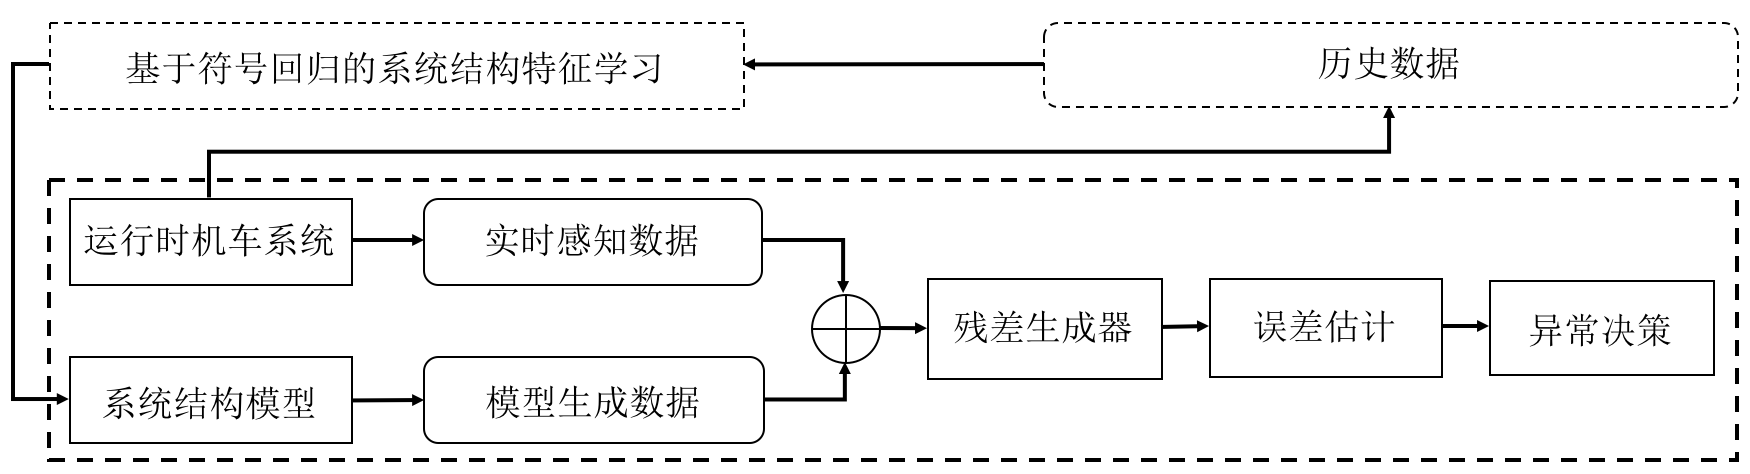
\includegraphics[scale=0.5]{figures/sr-anomaly-framework-application.png}
\caption{基于系统结构特征的在线实时异常检测框架}
\label{fig:sr-application}
\end{figure}

\section{实验结果与分析}
\label{sec:sr-experiment}

% 当年算法实验的参数
% 软件环境
% (1) myeclipse-10.0
% (2) jdk-7u7-windows-x64
% (3) windows7旗舰版,64bit
%  硬件环境
% (1) CPU:AMD A6-4455M (双核)
% (2) 主板:联想 Lenovo IdeaPad S405 (AMD A75/A70M (Hudson-D3/M3))
% (3) 内存:8 GBytes
% (4) 显卡:ATI/AMD Radeon HD 7500G, 512 MB of DDR3 SDRAM
% (5) 硬盘:希捷 ST500LT012-9WS142

实验硬件的主要参数:CPU,Intel(R) Xeon(R) CPU E5-2682,16核,2.50GHz;内存,235GB。代码使用 Python 3.6.0 实现,结合FFX和Deap工具包作为结构和参数学习引擎,FFX用于生成初始解,Deap用于对初始解进行剪枝。

数据采集自HXD3型电力机车,环境如图\ref{fig:sr-data-collect},数据说明见表\ref{tab:sr-variables}。本文在 1000 次正常运行过程中采集的数据集上进行交叉验证(针对一次运行,前50\%的数据作为训练集,后50\%作为验证集),学习6个轴温的结构特征,标号分别为 ZX\_WD\_1,ZX\_WD\_2,ZX\_WD\_3,ZX\_WD\_4,ZX\_WD\_5,ZX\_WD\_6。比如针对ZX\_WD\_1的学习,输入ZX\_WD\_1作为目标变量,因变量是表\ref{tab:sr-variables}中除了ZX\_WD\_1外的所有信号,初始基函数集定义为\ref{equ:sr-ops};对于Deap中遗传算法的参数,种群大小为500,突变率为50\%,交叉率为100\%;训练迭代次数是100次;评价指标定义为\ref{equ:sr-loss},$\lambda=1$,同时考虑误差因子和复杂度因子。

实验展示一次运行的结果。
\begin{itemize}
  \item 表\ref{tab:sr-ffx-1}至表\ref{tab:sr-ffx-6}给出了由 FFX 学习的最好的(得分最高的)8个结构特征,分别对应6个轴温数据。从实验结果可以看到,结构特征表达式具有一定的可解释性但仍相当复杂;并且训练误差和测试误都维持在较低的水平,说明结构特征对数据具有良好的拟合能力。图\ref{fig:ffx_zx_wd}给出了基于最优结构特征的模拟结果,针对每个轴温数据,给出了真实值、预测值和误差,可以看到由结构表达式生成的预测值对真实值具有较好的拟合效果。
  \item 表\ref{tab:sr-deap-1}至表\ref{tab:sr-deap-6}是经过 Deap剪枝后的结果,表中所列结构表达式为所有输出,可以看到相比于初始解,复杂度更低更便于理解,并且训练误差和测试误差都维持在较低水平。图\ref{fig:deap_zx_wd}给出了基于最优结构特征的模拟结果,相比于初始解能更好的表达数据的轨迹。
\end{itemize}

实验结果表明本文方法可有效学习多元信号间的线性/非线性关联关系,即结构特征;所学结构特征具有良好的解释性,对真实数据的运行轨迹具有很好的拟合效果。需要注意的是本文方法仍存在产生冗余运算子的情况,有进一步改进的空间,对此,Schmidt 等人已有初步尝试\cite{schmidt2009distilling},值得深入。

\begin{center}
\begin{longtable}[c]{p{9cm}<{\centering}*{3}{c}}
\caption{基于FFX针对ZX\_WD\_1学习的前8个最优结构特征}
\label{tab:sr-ffx-1}\\
\toprule[1.5pt]
模型 & 测试误差 & 训练误差 & 复杂度 \\\midrule[1pt]
\endfirsthead
\multicolumn{4}{c}{续表~\thetable\hskip1em 基于FFX针对ZX\_WD\_1学习的前8个最优结构特征}\\
\toprule[1.5pt]
模型 & 测试误差 & 训练误差 & 复杂度 \\\midrule[1pt]
\endhead
\hline
\multicolumn{4}{r}{续下页}
\endfoot
\endlastfoot
      35.0 & 1.354576 & 1.355095 & 0 \\
      $25.5 + 0.00904*ZX\_WD\_5 * ZX\_WD\_6$ & 0.913770 & 0.914579 & 1 \\
      $8.74 + 0.519*ZX\_WD\_6 + 0.291*ZX\_WD\_5$ & 0.753903 & 0.754591 & 2 \\
      $6.03 + 0.539*ZX\_WD\_6 + 0.332*ZX\_WD\_5 + 0.0223*ZX\_HW\_2$ & 0.694735 & 0.695431 & 3 \\
      $14.2 / (1.0 - 0.00703*ZX\_WD\_6 - 0.00690*ZX\_WD\_5 - 0.00302*ZX\_WD\_4 - 0.00103*ZX\_HW\_2)$ & 0.427490 & 0.427225 & 4 \\
      $(14.6 - 0.0243*ZX\_HW\_1) / (1.0 - 0.00706*ZX\_WD\_5 - 0.00704*ZX\_WD\_6 - 0.00297*ZX\_WD\_4 - 0.00125*ZX\_HW\_2)$ & 0.421005 & 0.420607 & 5 \\
      $-42.2 + 13.4*log10(ZX\_WD\_5) * log10(ZX\_WD\_6) + 9.72*log10(ZX\_WD\_5) * log10(ZX\_WD\_4) + 8.08*log10(ZX\_WD\_5) * log10(ZX\_HW\_2) + 0.691*log10(ZX\_WD\_2) * log10(ZX\_WD\_6) + 0.00511*ZX\_WD\_6^{2} - 0.00176*ZX\_HW\_1^{2}$ & 0.409125 & 0.409015 & 6 \\ 
      $32.6 - 0.557*max(0,33.2-ZX\_WD\_5) + 0.255*max(0,ZX\_WD\_6-31.3) - 0.235*max(0,36.0-ZX\_WD\_4) + 0.212*max(0,ZX\_WD\_6-30.8) - 0.131*max(0,36.1-ZX\_HW\_2) + 0.101*max(0,ZX\_WD\_5-32.0) + 0.0911*max(0,ZX\_WD\_6-31.9) + 0.0778*ZX\_WD\_6 + 0.0591*max(0,ZX\_WD\_2-37.6)$ & 0.397894 & 0.398467 & 9 \\
\bottomrule[1.5pt]
\end{longtable}
\end{center}

\begin{longtable}[c]{p{9cm}<{\centering}*{3}{c}}
\caption{基于FFX针对ZX\_WD\_2学习的前8个最优结构特征}\label{tab:sr-ffx-2}\\
\toprule[1.5pt]
模型 & 测试误差 & 训练误差 & 复杂度 \\\midrule[1pt]
\endfirsthead
\multicolumn{4}{c}{续表~\thetable\hskip1em 基于FFX针对ZX\_WD\_2学习的前8个最优结构特征}\\
\toprule[1.5pt]
模型 & 测试误差 & 训练误差 & 复杂度 \\\midrule[1pt]
\endhead
\hline
\multicolumn{4}{r}{续下页}
\endfoot
\endlastfoot
      37.5 & 1.249001 & 1.249430 & 0 \\
      $33.6 + 0.00339*ZX\_WD\_4 * ZX\_WD\_5$ & 1.114234 & 1.114899 & 1 \\
      $22.5 + 0.00923*ZX\_WD\_4 * ZX\_WD\_5 + 0.00380*ZX\_WD\_3 * ZX\_WD\_5$ & 0.842994 & 0.844262 & 2 \\
      $17.9 / (1.0 - 0.00748*ZX\_WD\_5 - 0.00444*ZX\_WD\_4 - 0.00341*ZX\_WD\_3)$ & 0.806176 & 0.807632 & 3 \\
      $20.9 + 0.00870*ZX\_WD\_4 * ZX\_WD\_5 + 0.00399*ZX\_WD\_3 * ZX\_WD\_5 + 0.00286*ZX\_WD\_4 * ZX\_HW\_2 - 3.78e-6*ZD\_TFG^{2}$ & 0.757751 & 0.759322 & 4 \\
      $-15.2 + 13.8*log10(ZX\_WD\_5) * log10(ZX\_WD\_4) + 7.53*log10(ZX\_WD\_5) * log10(ZX\_WD\_3) + 0.00250*ZX\_HW\_2^{2} + 0.00147*ZX\_WD\_4^{2} - 5.22e-6*ZD\_TFG^{2}$ & 0.740418 & 0.741918 & 5 \\
      $-14.2 + 13.1*log10(ZX\_WD\_5) * log10(ZX\_WD\_4) + 7.59*log10(ZX\_WD\_5) * log10(ZX\_WD\_3) + 0.00293*ZX\_HW\_2^{2} + 0.00163*ZX\_WD\_4^{2} - 0.000125*ZD\_JHG - 5.62e-6*ZD\_TFG^{2}$ & 0.734446 & 0.735908 & 6 \\
      $20.5 + 0.00813*ZX\_WD\_4 * ZX\_WD\_5 + 0.00373*ZX\_WD\_3 * ZX\_WD\_5 + 0.00320*ZX\_WD\_4 * ZX\_HW\_2 + 0.00108*ZX\_HW\_2^{2} + 0.000383*ZX\_WD\_3 * ZX\_HW\_2 - 0.000157*ZD\_JHG - 5.69e-6*ZD\_TFG^{2}$ & 0.731474 & 0.732970 & 7 \\ 
\bottomrule[1.5pt]
\end{longtable}

\begin{longtable}[c]{p{9cm}<{\centering}*{3}{c}}
\caption{基于FFX针对ZX\_WD\_3学习的前8个最优结构特征}\label{tab:sr-ffx-3}\\
\toprule[1.5pt]
模型 & 测试误差 & 训练误差 & 复杂度 \\\midrule[1pt]
\endfirsthead
\multicolumn{4}{c}{续表~\thetable\hskip1em 基于FFX针对ZX\_WD\_3学习的前8个最优结构特征}\\
\toprule[1.5pt]
模型 & 测试误差 & 训练误差 & 复杂度 \\\midrule[1pt]
\endhead
\hline
\multicolumn{4}{r}{续下页}
\endfoot
\endlastfoot
      36.6 & 0.949297 & 0.949557 & 0 \\
      $6.55 + 0.843*ZX\_WD\_4$ & 0.402844 & 0.401142 & 1 \\
      $4.39 + 0.878*ZX\_WD\_4 + 0.0282*ZX\_HW\_1$ & 0.395118 & 0.393432 & 2 \\
      $(19.0 - 0.00995*ZX\_WD\_5) / (1.0 - 0.0125*ZX\_WD\_4 - 0.00135*ZX\_HW\_1)$ & 0.393192 & 0.391551 & 3 \\
      $(19.4 - 0.0342*ZX\_WD\_5) / (1.0 - 0.0123*ZX\_WD\_4 - 0.00169*ZX\_HW\_1 - 0.000162*ZX\_WD\_2)$ & 0.389710 & 0.388109 & 4 \\
      $4.12 + 0.891*ZX\_WD\_4 + 0.0744*ZX\_HW\_1 - 0.0733*ZX\_WD\_5 + 0.0177*ZX\_WD\_2 - 0.00114*ZD\_LLJ$ & 0.386751 & 0.385115 & 5 \\
      $17.7 / (1.0 - 0.0122*ZX\_WD\_4 - 0.00192*ZX\_HW\_1 - 0.00125*max(0,33.6-ZX\_WD\_5) - 0.000561*max(0,35.9-ZX\_WD\_1) - 0.000312*ZX\_WD\_2 - 0.000132*ZX\_WD\_6)$ & 0.385381 & 0.383703 & 6 \\
      $3.51 + 0.920*ZX\_WD\_4 + 0.126*ZX\_HW\_1 - 0.120*ZX\_WD\_5 + 0.0374*ZX\_WD\_2 - 0.0306*ZX\_HW\_2 - 0.00734*ZX\_WD\_1 - 0.00178*ZD\_LLJ$ & 0.381686 & 0.380206 & 7 \\
\bottomrule[1.5pt]
\end{longtable}

\begin{longtable}[c]{p{9cm}<{\centering}*{3}{c}}
\caption{基于FFX针对ZX\_WD\_4学习的前8个最优结构特征}\label{tab:sr-ffx-4}\\
\toprule[1.5pt]
模型 & 测试误差 & 训练误差 & 复杂度 \\\midrule[1pt]
\endfirsthead
\multicolumn{4}{c}{续表~\thetable\hskip1em 基于FFX针对ZX\_WD\_4学习的前8个最优结构特征}\\
\toprule[1.5pt]
模型 & 测试误差 & 训练误差 & 复杂度 \\\midrule[1pt]
\endhead
\hline
\multicolumn{4}{r}{续下页}
\endfoot
\endlastfoot
     35.6 & 0.930301 & 0.931435 & 0 \\
      $23.4 + 0.333*ZX\_WD\_3$ & 0.656427 & 0.657099 & 1 \\
      $21.0 + 0.218*ZX\_WD\_3 * log10(ZX\_WD\_1) + 0.00185*ZX\_HW\_2 * ZX\_WD\_3$ & 0.453389 & 0.453613 & 2 \\
      $16.3 + 0.260*ZX\_WD\_3 * log10(ZX\_WD\_1) + 0.00299*ZX\_HW\_2 * ZX\_WD\_3 + 0.000653*ZX\_WD\_3^{2}$ & 0.335498 & 0.335179 & 3 \\
      $3.34 + 0.610*ZX\_WD\_3 + 0.124*ZX\_HW\_2 + 0.108*ZX\_WD\_1 + 0.0504*ZX\_WD\_2$ & 0.308872 & 0.308640 & 4 \\
      $13.0 + 1.68*log10(ZX\_WD\_3) * log10(ZX\_WD\_1) + 0.173*ZX\_WD\_3 * log10(ZX\_WD\_1) + 0.00352*ZX\_HW\_2 * ZX\_WD\_3 + 0.00258*ZX\_WD\_3^{2} + 0.000618*ZX\_WD\_2^{2}$ & 0.308366 & 0.308182 & 5 \\
      $3.26 + 0.616*ZX\_WD\_3 + 0.132*ZX\_HW\_2 + 0.113*ZX\_WD\_1 + 0.0526*ZX\_WD\_2 - 0.0209*ZX\_HW\_1 + 0.000356*ZD\_LLJ$ & 0.307278 & 0.307066 & 6 \\
      $3.36 + 0.621*ZX\_WD\_3 + 0.143*ZX\_HW\_2 + 0.117*ZX\_WD\_1 + 0.0538*ZX\_WD\_2 - 0.0464*ZX\_HW\_1 - 0.000745*ZD\_SPEED + 0.000611*ZD\_LLJ$ & 0.306412 & 0.306220 & 7 \\
\bottomrule[1.5pt]
\end{longtable}

\begin{longtable}[c]{p{9cm}<{\centering}*{3}{c}}
\caption{基于FFX针对ZX\_WD\_5学习的前8个最优结构特征}\label{tab:sr-ffx-5}\\
\toprule[1.5pt]
模型 & 测试误差 & 训练误差 & 复杂度 \\\midrule[1pt]
\endfirsthead
\multicolumn{4}{c}{续表~\thetable\hskip1em 基于FFX针对ZX\_WD\_5学习的前8个最优结构特征}\\
\toprule[1.5pt]
模型 & 测试误差 & 训练误差 & 复杂度 \\\midrule[1pt]
\endhead
\hline
\multicolumn{4}{r}{续下页}
\endfoot
\endlastfoot
     32.1 & 0.868038 & 0.867657 & 0 \\
      $22.2 + 0.283*ZX\_WD\_1$ & 0.571645 & 0.571623 & 1 \\
      $18.5 + 0.330*ZX\_WD\_1 + 0.0625*ZX\_HW\_1$ & 0.503551 & 0.503674 & 2 \\
      $18.3 / (1.0 - 0.00542*ZX\_WD\_1 - 0.00493*ZX\_HW\_1 - 0.00213*ZX\_WD\_2)$ & 0.409921 & 0.410352 & 3 \\
      $31.4 + 0.316*max(0,ZX\_WD\_1-33.8) + 0.141*max(0,ZX\_HW\_1-32.3) + 0.129*max(0,ZX\_WD\_1-34.3) + 0.121*max(0,ZX\_HW\_1-31.8)$ & 0.398462 & 0.398821 & 4 \\
      $31.4 + 0.318*max(0,ZX\_WD\_1-33.8) + 0.222*max(0,ZX\_HW\_1-32.3) + 0.145*max(0,ZX\_WD\_1-34.3) + 0.0893*max(0,ZX\_HW\_1-31.8) - 0.0554*max(0,36.8-ZX\_WD\_2)$ & 0.377175 & 0.377608 & 5 \\
      $17.3 / (1.0 - 0.00577*ZX\_WD\_1 - 0.00521*ZX\_HW\_1 - 0.00403*max(0,35.0-ZX\_WD\_4) - 0.00299*max(0,33.3-ZX\_HW\_2) - 0.00143*ZX\_WD\_2 - 0.00107*ZX\_WD\_6)$ & 0.354132 & 0.354684 & 6 \\
      $31.4 + 0.342*max(0,ZX\_WD\_1-33.8) + 0.223*max(0,ZX\_HW\_1-32.3) + 0.146*max(0,32.3-ZX\_HW\_2) + 0.118*max(0,ZX\_HW\_1-31.8) + 0.106*max(0,ZX\_WD\_1-34.3) - 0.0740*max(0,36.8-ZX\_WD\_2) + 0.0600*max(0,35.0-ZX\_WD\_4) - 0.0396*max(0,36.5-ZX\_WD\_1)$ & 0.349669 & 0.350131 & 8 \\
\bottomrule[1.5pt]
\end{longtable}

\begin{longtable}[c]{p{9cm}<{\centering}*{3}{c}}
\caption{基于FFX针对ZX\_WD\_6学习的前8个最优结构特征}\label{tab:sr-ffx-6}\\
\toprule[1.5pt]
模型 & 测试误差 & 训练误差 & 复杂度 \\\midrule[1pt]
\endfirsthead
\multicolumn{4}{c}{续表~\thetable\hskip1em 基于FFX针对ZX\_WD\_6学习的前8个最优结构特征}\\
\toprule[1.5pt]
模型 & 测试误差 & 训练误差 & 复杂度 \\\midrule[1pt]
\endhead
\hline
\multicolumn{4}{r}{续下页}
\endfoot
\endlastfoot
    32.5 & 0.895700 & 0.895482 & 0 \\
      $24.2 + 0.239*ZX\_WD\_1$ & 0.619888 & 0.619435 & 1 \\
      $20.2 + 0.300*ZX\_WD\_1 + 0.0527*ZX\_HW\_2$ & 0.511317 & 0.510716 & 2 \\
      $11.3 + 0.388*ZX\_WD\_1 + 0.122*ZX\_HW\_1 + 0.108*ZX\_HW\_2$ & 0.363861 & 0.362749 & 3 \\
      $8.84 + 0.404*ZX\_WD\_1 + 0.147*ZX\_HW\_1 + 0.112*ZX\_HW\_2 + 0.0257*ZX\_WD\_3$ & 0.351119 & 0.350121 & 4 \\
      $20.6 + 0.00430*ZX\_HW\_1 * ZX\_WD\_1 + 0.00323*ZX\_HW\_2 * ZX\_WD\_1 + 0.00161*ZX\_WD\_1^{2} + 0.000915*ZX\_WD\_3 * ZX\_WD\_1 + 4.54e-8*ZD\_JHG^{2}$ & 0.350564 & 0.349649 & 5 \\
      $8.45 + 0.407*ZX\_WD\_1 + 0.152*ZX\_HW\_1 + 0.110*ZX\_HW\_2 + 0.0309*ZX\_WD\_3 + 0.000971*ZD\_SPEED + 0.000796*ZD\_LLJ$ & 0.349222 & 0.348054 & 6 \\
      $8.37 + 5.21*log10(ZX\_HW\_1) * log10(ZX\_HW\_2) + 2.64*log10(ZX\_HW\_1) * log10(ZX\_WD\_3) - 0.959*log10(ZX\_WD\_2) + 0.00596*ZX\_WD\_1^{2} + 0.00206*ZD\_SPEED + 0.00197*ZD\_LLJ + 2.25e-7*ZD\_LCG^{2}$ & 0.344627 & 0.343397 & 7 \\
\bottomrule[1.5pt]
\end{longtable}

\begin{longtable}[c]{p{4.3cm}<{\centering}p{4.3cm}<{\centering}*{3}{c}}
\caption{基于Deep剪枝后的ZX\_WD\_1最优结构特征}\label{tab:sr-deap-1}\\
\toprule[1.5pt]
原模型 & 简化模型 & 测试误差 & 训练误差 &  复杂度\\\midrule[1pt]
\endfirsthead
\multicolumn{5}{c}{续表~\thetable\hskip1em 基于Deep剪枝后的ZX\_WD\_1最优结构特征}\\
\toprule[1.5pt]
原模型 & 简化模型 & 测试误差 & 训练误差 &  复杂度 \\\midrule[1pt]
\endhead
\hline
\multicolumn{5}{r}{续下页}
\endfoot
\endlastfoot
      sqrt(ZD\_TFG) & $sqrt(ZD\_TFG)$ & 10.039514 & 10.036110 & 2 \\
      Add(2.422, ZX\_WD\_6) & $ZX\_WD\_6 + 2.422$ & 0.670062 & 0.670128 & 3 \\
      Sub(ZX\_WD\_4, cos(ZX\_WD\_5)) & $ZX\_WD\_4 - cos(ZX\_WD\_5)$ & 0.643303 & 0.642128 & 4 \\
\bottomrule[1.5pt]
\end{longtable}

\begin{longtable}[c]{p{4.3cm}<{\centering}p{4.3cm}<{\centering}*{3}{c}}
\caption{基于Deep剪枝后的ZX\_WD\_2最优结构特征}\label{tab:sr-deap-2}\\
\toprule[1.5pt]
原模型 & 简化模型 & 测试误差 & 训练误差 &  复杂度\\\midrule[1pt]
\endfirsthead
\multicolumn{5}{c}{续表~\thetable\hskip1em 基于Deep剪枝后的ZX\_WD\_2最优结构特征}\\
\toprule[1.5pt]
原模型 & 简化模型 & 测试误差 & 训练误差 &  复杂度 \\\midrule[1pt]
\endhead
\hline
\multicolumn{5}{r}{续下页}
\endfoot
\endlastfoot
      sqrt(ZD\_TFG) & $sqrt(ZD\_TFG)$ & 12.576153 & 12.572426 & 2 \\
      Add(1.0, ZX\_WD\_3) & $ZX\_WD\_3 + 1.0$ & 0.981440 & 0.981503 & 3 \\
      Add(ZX\_WD\_3, 1.0) & $ZX\_WD\_3 + 1.0$ & 0.981440 & 0.981503 & 3 \\
      Add(ZX\_WD\_5, sqrt(ZX\_WD\_5)) & $sqrt(ZX\_WD\_5) + ZX\_WD\_5$ & 0.953105 & 0.953624 & 4 \\
      Add(sqrt(ZX\_WD\_5), ZX\_WD\_5)  & $sqrt(ZX\_WD\_5) + ZX\_WD\_5$ & 0.953105 & 0.953624 & 4 \\
\bottomrule[1.5pt]
\end{longtable}

\begin{longtable}[c]{p{4.3cm}<{\centering}p{4.3cm}<{\centering}*{3}{c}}
\caption{基于Deep剪枝后的ZX\_WD\_3最优结构特征}\label{tab:sr-deap-3}\\
\toprule[1.5pt]
原模型 & 简化模型 & 测试误差 & 训练误差 &  复杂度\\\midrule[1pt]
\endfirsthead
\multicolumn{5}{c}{续表~\thetable\hskip1em 基于Deep剪枝后的ZX\_WD\_3最优结构特征}\\
\toprule[1.5pt]
原模型 & 简化模型 & 测试误差 & 训练误差 &  复杂度 \\\midrule[1pt]
\endhead
\hline
\multicolumn{5}{r}{续下页}
\endfoot
\endlastfoot
      sqrt(ZD\_TFG) & $sqrt(ZD\_TFG)$ & 11.578368 & 11.573686 & 2 \\
      Add(ZX\_WD\_4, 1.0) & $ZX\_WD\_4 + 1.0$ & 0.402275 & 0.400682 & 3 \\
      Add(1.0, ZX\_WD\_4) & $ZX\_WD\_4 + 1.0$ & 0.402275 & 0.400682 & 3 \\
\bottomrule[1.5pt]
\end{longtable}

\begin{longtable}[c]{p{4.3cm}<{\centering}p{4.3cm}<{\centering}*{3}{c}}
\caption{基于Deep剪枝后的ZX\_WD\_4最优结构特征}\label{tab:sr-deap-4}\\
\toprule[1.5pt]
原模型 & 简化模型 & 测试误差 & 训练误差 &  复杂度\\\midrule[1pt]
\endfirsthead
\multicolumn{5}{c}{续表~\thetable\hskip1em 基于Deep剪枝后的ZX\_WD\_4最优结构特征}\\
\toprule[1.5pt]
原模型 & 简化模型 & 测试误差 & 训练误差 &  复杂度 \\\midrule[1pt]
\endhead
\hline
\multicolumn{5}{r}{续下页}
\endfoot
\endlastfoot
      sqrt(ZD\_TFG) & $sqrt(ZD\_TFG)$ & 10.619709 & 10.616273 & 2 \\
      Add(3.0450, ZX\_WD\_6) & $ZX\_WD\_6 + 3.0450$ & 0.633333 & 0.633819 & 3 \\
      sqrt(Mul(ZX\_WD\_3, ZX\_HW\_2)) & $sqrt(ZX\_HW\_2*ZX\_WD\_3)$ & 0.435390 & 0.435666 & 4 \\
      Add(cos(log(ZX\_WD\_3)), ZX\_WD\_3) & $ZX\_WD\_3 + cos(log(ZX\_WD\_3))$ & 0.409323 & 0.407365 & 5 \\
      Sub(ZX\_WD\_3, cos(Div(ZX\_WD\_3, ZD\_JHG))) & $ZX\_WD\_3 - cos(ZX\_WD\_3/ZD\_JHG)$ & 0.407747 & 0.403063 & 6 \\
\bottomrule[1.5pt]
\end{longtable}

\begin{longtable}[c]{p{5cm}<{\centering}p{4.3cm}<{\centering}*{3}{c}}
\caption{基于Deep剪枝后的ZX\_WD\_5最优结构特征}\label{tab:sr-deap-5}\\
\toprule[1.5pt]
原模型 & 简化模型 & 测试误差 & 训练误差 &  复杂度\\\midrule[1pt]
\endfirsthead
\multicolumn{5}{c}{续表~\thetable\hskip1em 基于Deep剪枝后的ZX\_WD\_5最优结构特征}\\
\toprule[1.5pt]
原模型 & 简化模型 & 测试误差 & 训练误差 &  复杂度 \\\midrule[1pt]
\endhead
\hline
\multicolumn{5}{r}{续下页}
\endfoot
\endlastfoot
      sqrt(ZD\_TFG) & $sqrt(ZD\_TFG)$ & 7.196478 & 7.190211 & 2 \\
      Add(-0.4640, ZX\_WD\_6) & $ZX\_WD\_6 - 0.4640$ & 0.607207 & 0.607687 & 3 \\
      Add(ZX\_WD\_6, log(cos(sin(log(cos(ZD\_TFG)))))) & $ZX\_WD\_6 + log(cos(sin(log(cos(ZD\_TFG)))))$ & 0.594462 & 0.595329 & 9 \\
\bottomrule[1.5pt]
\end{longtable}

\begin{longtable}[c]{p{4cm}<{\centering}p{5.2cm}<{\centering}*{3}{c}}
\caption{基于Deep剪枝后的ZX\_WD\_6最优结构特征}\label{tab:sr-deap-6}\\
\toprule[1.5pt]
原模型 & 简化模型 & 测试误差 & 训练误差 &  复杂度\\\midrule[1pt]
\endfirsthead
\multicolumn{5}{c}{续表~\thetable\hskip1em 基于Deep剪枝后的ZX\_WD\_6最优结构特征}\\
\toprule[1.5pt]
原模型 & 简化模型 & 测试误差 & 训练误差 &  复杂度 \\\midrule[1pt]
\endhead
\hline
\multicolumn{5}{r}{续下页}
\endfoot
\endlastfoot
      sqrt(ZD\_TFG) & $sqrt(ZD\_TFG)$ & 7.613762 & 7.609814 & 2 \\
      Mul(ZX\_WD\_1, 0.9300) & $0.9300*ZX\_WD\_1$ & 0.595735 & 0.595721 & 3 \\
\bottomrule[1.5pt]
\end{longtable}

\begin{figure}[H]
\centering
\begin{subfigure}[t]{0.48\textwidth}
    \centering
    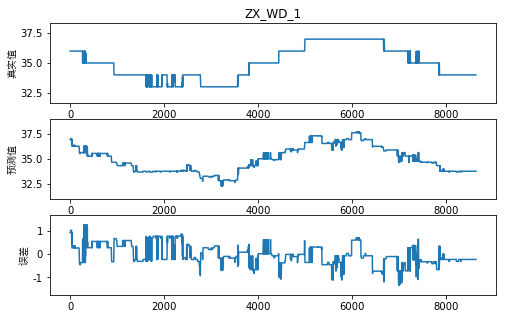
\includegraphics[scale=0.45]{figures/sr/ffx-zx_wd_1.png}
    %\caption{ZX\_WD\_1}
\end{subfigure}\hfill
\begin{subfigure}[t]{0.48\textwidth}
    \centering
    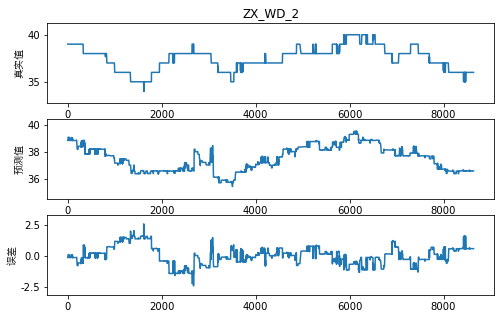
\includegraphics[scale=0.45]{figures/sr/ffx-zx_wd_2.png}
    %\caption{ZX\_WD\_2}
\end{subfigure}\\
\begin{subfigure}[t]{0.48\textwidth}
  \centering
  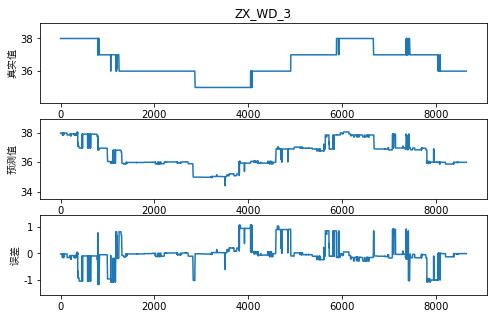
\includegraphics[scale=0.45]{figures/sr/ffx-zx_wd_3.png}
  %\caption{ZX\_WD\_3}
\end{subfigure}\hfill
\begin{subfigure}[t]{0.48\textwidth}
    \centering
    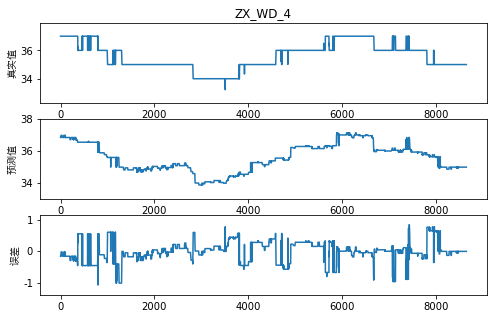
\includegraphics[scale=0.45]{figures/sr/ffx-zx_wd_4.png}
    %\caption{ZX\_WD\_4}
\end{subfigure}\\
\begin{subfigure}[t]{0.48\textwidth}
  \centering
  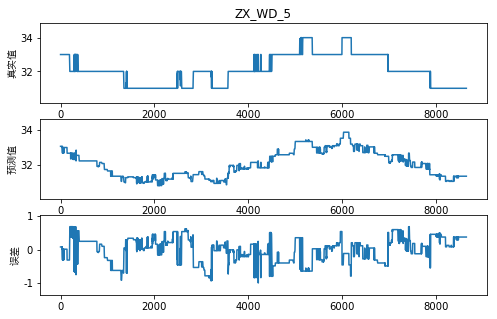
\includegraphics[scale=0.45]{figures/sr/ffx-zx_wd_5.png}
  %\caption{ZX\_WD\_5}
\end{subfigure}\hfill
\begin{subfigure}[t]{0.48\textwidth}
    \centering
    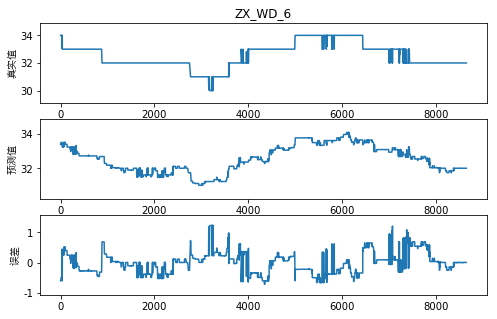
\includegraphics[scale=0.45]{figures/sr/ffx-zx_wd_6.png}
    %\caption{ZX\_WD\_6}
\end{subfigure}
\caption{基于FFX所学最优结构特征的模拟结果}
\label{fig:ffx_zx_wd}
\end{figure}

\begin{figure}[H]
\centering
\begin{subfigure}[t]{0.48\textwidth}
    \centering
    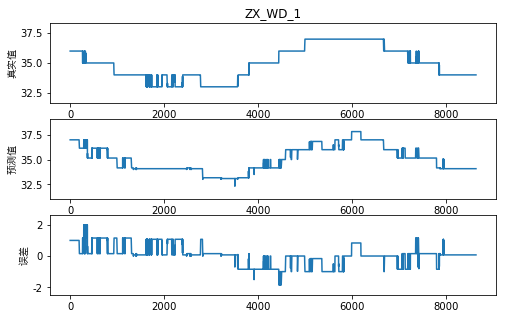
\includegraphics[scale=0.45]{figures/sr/deap-zw_wd_1.png}
    %%\caption{ZX\_WD\_1}
\end{subfigure}\hfill
\begin{subfigure}[t]{0.48\textwidth}
    \centering
    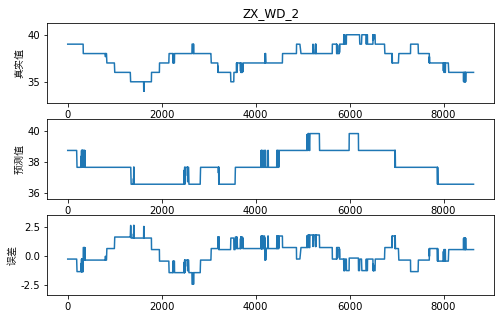
\includegraphics[scale=0.45]{figures/sr/deap-zw_wd_2.png}
    %%\caption{ZX\_WD\_2}
\end{subfigure}\\
\begin{subfigure}[t]{0.48\textwidth}
  \centering
  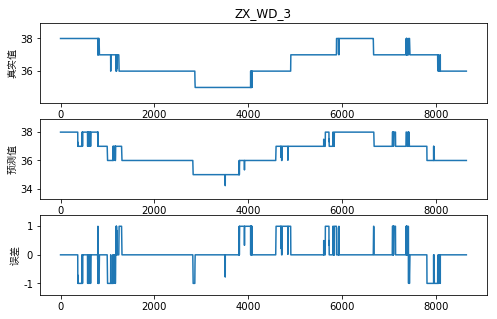
\includegraphics[scale=0.45]{figures/sr/deap-zw_wd_3.png}
  %%\caption{ZX\_WD\_3}
\end{subfigure}\hfill
\begin{subfigure}[t]{0.48\textwidth}
    \centering
    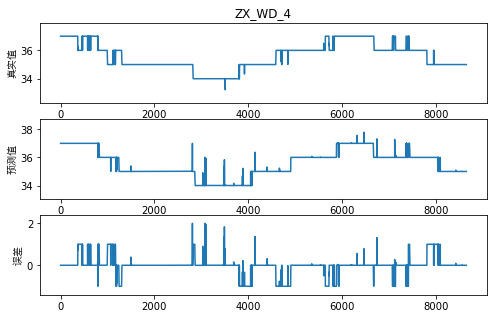
\includegraphics[scale=0.45]{figures/sr/deap-zw_wd_4.png}
    %%\caption{ZX\_WD\_4}
\end{subfigure}\\
\begin{subfigure}[t]{0.48\textwidth}
  \centering
  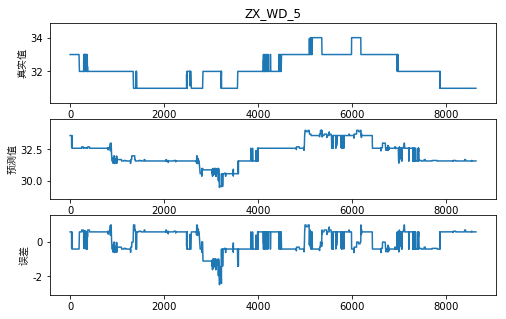
\includegraphics[scale=0.45]{figures/sr/deap-zw_wd_5.png}
  %%\caption{ZX\_WD\_5}
\end{subfigure}\hfill
\begin{subfigure}[t]{0.48\textwidth}
    \centering
    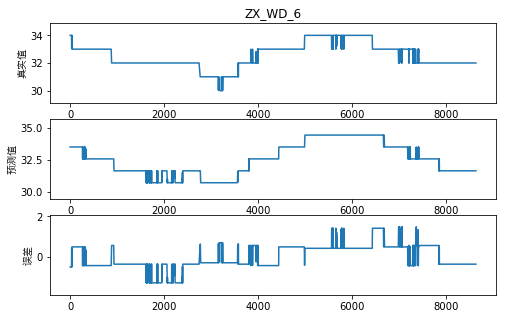
\includegraphics[scale=0.45]{figures/sr/deap-zw_wd_6.png}
    %%\caption{ZX\_WD\_6}
\end{subfigure}
\caption{基于Deap所学最优结构特征的模拟结果}
\label{fig:deap_zx_wd}
\end{figure}

\section{小结}

本章针对轴温为代表的设备正常状态数据开展机理挖掘研究。首先进行数据采集、预处理和分析工作。然后提出基于符号回归的系统结构特征学习方法,实验结果表明,所学结构特征具有很好的可解释性,表达了多元信号间的相互作用关系。最后将最优系统结构模型作为系统运行时的健康基线,设计了在线实时异常检测框架。实验结果表明系统结构模型对真实数据的运行轨迹具有很好的拟合能力,可作为系统正常状态的基准。值得一提的是基于符号回归的系统结构特征学习方法还支持了本文第\ref{chap:critical-transection}章的动态系统稳定性分析。


% !TEX root = ../main.tex

\chapter{基于临界相变理论的早期预警特征学习与应用}
\label{chap:critical-transection}

\section{引言}

% 临界相变的普适性,早期预警特征的存在性和普遍性
在社会生态系统中越来越普遍认为临界相变预示着复杂系统状态的急剧转变,其潜在灾难性可能导致复杂系统崩溃\cite{scheffer2009critical,scheffer2012anticipating}。尽管临界相变很难被预测,但由于全球都在关注生态系统的可持续发展,因此已有很多致力于识别临界相变早期预警特征的研究。近年来诸多研究已见证基于时间序列分析识别早期预警特征的可行性与有效性\cite{scheffer2009early,wang2012flickering,boettiger2012quantifying}。越来越多研究认识到多种复杂系统,比如生态\cite{scheffer2001catastrophic,rietkerk2004self,carpenter2011early}、哺乳动物的皮质神经元\cite{meisel2015critical}、气候\cite{lenton2008tipping}和经济市场\cite{may2008complex}等复杂系统,临近临界相变点时受到轻微扰动后很难恢复到平衡状态,并且表现如临界慢化现象\cite{scheffer2009early}和偏斜度增加\cite{guttal2008changing}这样的早期预警特征。

% 早期预警指标的潜在原因
复杂动态系统在临近一个特定域值时将会经历临界相变\cite{ladyman2013complex},这样的临界点存在是动态系统固有的非线性和随机性导致的结果\cite{bar1997dynamics,endy2005foundations}。虽然工业系统似乎与生态系统有所不同,但类似于喷气发动机,机车和轴承这样的系统都属于动态系统,并且在复杂的内部因素和环境因素相互作用下表现出非线性和随机波动性\cite{strogatz2018nonlinear,cotilla2012predicting}。比如由于车轮裂纹过度疲劳引起的德国高速列车重大事故\cite{oestern2000facts},直观地来看裂纹加快恶化以至于脱轨事件发生的过程与自然系统的临界相变非常相似。

% 工业系统面临的挑战
在工业系统中发现潜在故障极其具有挑战性。虽然系统的设计都基于定义良好的物理方程,然而系统内部组件之间和系统与工作环境之间存在复杂关系以至于很难甚至不可能穷尽所有的解析模型\cite{chan2007data},即使可以通过故障物理机制或可靠性分析来识别失效过程,但真实的工作状态和工作环境也很难完全复现。再者,生产过程的全球化成为了全面理解领域知识的阻碍,工业系统故障预测问题仍然是全球范围内的挑战。因此学习对领域知识依赖更少甚至不依赖的有效且通用的失效早期预警特征十分具有吸引力。

% 本文工作,这里要高度概括,放到设计部分。
综上所述,本文引入基于临界相变的状态分析理论,提出系统失效早期预警特征学习方法,并基于此提出关键跳变检测算法预测系统失效,此过程只需依赖少量失效敏感时间序列,可有效应对故障数据小样本、不完备特性的挑战。

\section{总体框架}
\label{sec:csd-framework}

如图\ref{fig:csd-framework},本章的总体内容结构,分为特征学习和特征应用两部分。其中特征学习包括随机波动信号挖掘、系统早期预警特征学习、系统失效与临界相变一致性检验。

(1)原生时间序列

本文基于4个来自不同系统的数据集展开研究和应用工作,这些系统包括柴油机车的制动管(气动系统),涡轮发动机(机械电子系统),IGBT(电力电子系统)和滚动轴承(机械系统)。柴油机车的制动管数据采集自本文所依托项目的商业运营机车,剩下的3个数据集是NASA预测卓越中心公开的基准数据集\cite{nasa2018}。所有的数据集都是通过传感器在系统从正常运行到失效过程中采集的单元或多元时间序列。详细介绍参见\ref{sec:csd-dataset}。

本文对数据及基于此的操作进行如下定义:以小写字母$x,y,z,...$表示时间序列。采样长度为\emph{n}的时间序列可表示为$x=\{x_{1}, x_{2}, ..., x_{n}\}$,其中$\{1,2,3,...,n\}$为下标也可看成采样时间点。$x_{t}$表示时刻$t$的观察值。$x(t)$表示从时刻\emph{t}开始到时间序列\emph{x}结尾的子序列。特别的当进行多子序列讨论时,比如对于任意整数 $i,j$ 并且$1 \leqslant  i,j \leqslant n, i \neq j$,有子序列$x(i),x(j)$,此时$x(i),x(j)$自动对齐,即较长的子序列从后往前进行截断以保证与较短子序列的长度一致,形式化的定义如下,不失一般性假设$i<j$,令$k=j-i$,那么$x(i)=\{x_{i}, ..., x_{n-k}\}, x(j) = \{x_{j}, ..., x_{n}\}$。

(2)随机波动信号挖掘

%传感器信号是以离散方式采集的时间序列,往往是一个或多个观测信号叠加的结果。
在复杂生态系统中,去趋势\cite{wang2012flickering}的操作通常用于抽取时间序列的随机波动部分以支持早期预警特征分析\cite{cotilla2012predicting}。基于时间序列的可列可加性,本文设计了随机波动信号挖掘(Fluctuation Mining, FM)框架,以保证提取的随机波动信号不存在与系统设计操作的直接关联性。首先对时间序列中的多个工作态进行识别与分离,然后通过相关性分析和/或少量专家知识识别失效敏感的工作态信号,最后通过物理方程或统计方程对操作趋势进行拟合剥离,而余下成分通过验证后则为系统固有随机波动信号。详细介绍参见\ref{sec:fluctuation-mining}。

(3) 系统失效早期预警特征学习

基于上一步挖掘的系统固有随机波动信号以及“系统失效与复杂系统临界相变一致”的假设,进行系统失效早期预警特征学习,研究早期预警特征是否可以被发现。首先基于系统的随机波动信号计算反应时间序列特性的滑动方差(Variance)、滑动自相关(Autocorrelation(1))和滑动偏斜度(Skewness);然后采用肯德尔(Kendall)趋势检验和敏感性分析进行有效性和鲁棒性进行检验。
详细介绍参见\ref{sec:csd-early-warning-mining}。
% 实验结果显示:所有系统,虽然属于不同工程系统类别,但临近失效过程中一致出现了CSD和偏斜度增加的早期预警特征,暗示了早期预警特征可作为系统失效的前兆。

(4) 系统失效与临界相变一致性检验

基于系统的原生时间序列检验假设——“系统失效与复杂系统临界相变一致”。若威尔科克森检验(Wilcoxon test)\cite{bisgaard2011time}、核密度估计\cite{bisgaard2011time}、基于赤池信息量准则(Akaike Information Criterion, AIC)的ARIMA模型分析和动态系统稳定性分析\cite{brunton2016discovering}均验证系统失效前后发生状态变迁,则证明系统失效与临界相变是一致的。详细介绍参见\ref{sec:csd-existence-test}。
% 实验结果表明被研究的系统在失效过程中确实经历了状态的突然转变,强有力的证明了工程系统失效和临界相变的一致性,进一步证明临界相变早期预警特征对系统失效预测的适用性。

(5) 系统失效(临界相变)早期预警特征应用

验证早期预警特征的存在性、有效性以及通用性之后,本文将系统失效(临界相变)早期预警特征统一称为{\heiti 系统失效早期预警特征},并将其应用到故障诊断、故障预测、状态监控和可视化展示等任务中。详细介绍参见\ref{sec:csd-application}。

\begin{figure}[H]
\centering
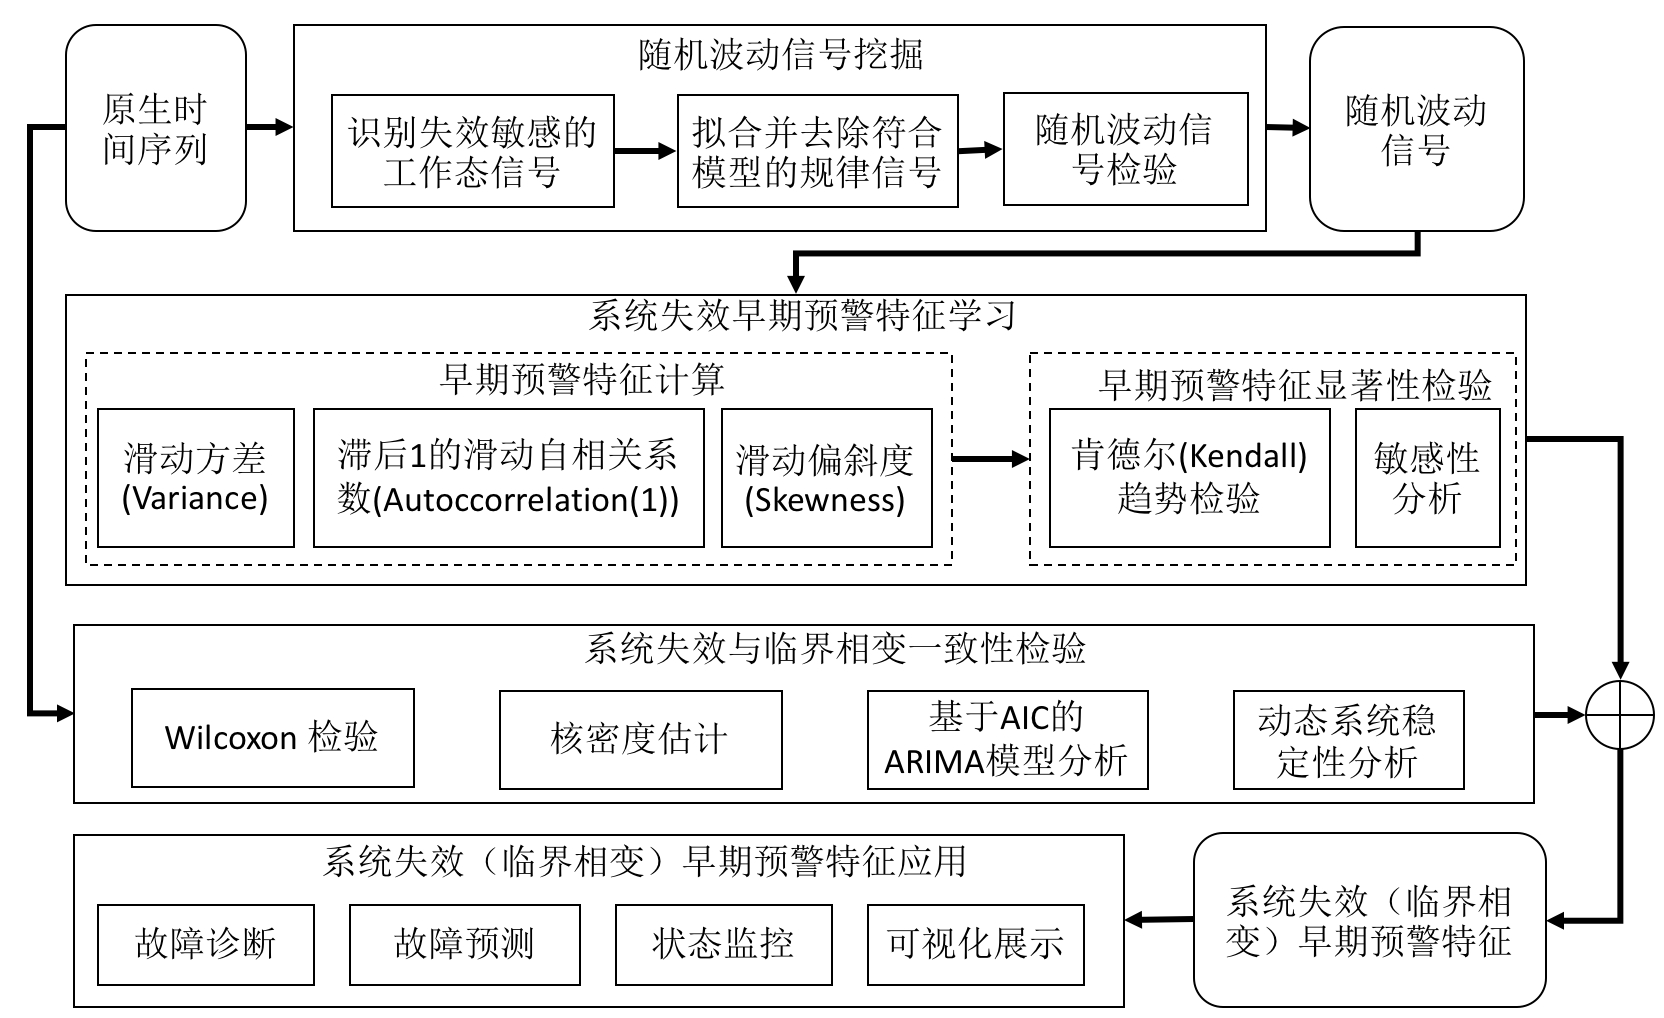
\includegraphics[scale=0.5]{csd-framework.png}
\caption{基于临界相变理论的早期预警特征学习、验证及应用的框架}
\label{fig:csd-framework}
\end{figure}

\section{系统失效早期预警特征学习}
\label{sec:csd-feature}

\subsection{随机波动信号挖掘}
\label{sec:fluctuation-mining}

通过传感器采集的时间序列常常存在多态性,即多个工作态混合(如图\ref{fig:fm-main-example}所示的信号明显存在两个工态,红色矩形标出),其中包含了对失效敏感的模式和非失效敏感的模式。基于时间序列的可列可加性,可以对时间序列进行如图\ref{fig:fm-main-structure}所示的拆分,分为符合某种或某几种模型的规律信号和受系统不确定性和环境等复杂因素影响的随机波动信号(又可称为残差)。随机波动信号挖掘具体分为以下两步:

(1)规律信号识别:规律信号的识别方法可以分为通用方法和领域相关方法。(a)通用方法基于规律信号满足某种通用方程的假设对时间序列进行拟合学习,比如多项式回归\ref{equ:fit-multiple-regression};高斯核回归\ref{equ:fit-gausian-regression},其中\emph{K}是带宽为\emph{h}的核函数,带宽\emph{h}往往是需要选择的重要参数,\emph{x}为输入,\emph{y}为输出;自回归\ref{equ:fit-autocorrelation}等。(b) 领域相关的方法,首先通过先验知识获取规律信号的运动方程,比如本文通过专家得知图\ref{fig:fm-main-example}中低态信号每个周期的运动满足等式\ref{equ:fit-real-example},然后基于此进行参数学习以拟合规律信号。通常情况下,领域相关的模型效果更好,但当先验知识缺乏时通用模型也可提供良好支持。
\begin{subequations}
\begin{align}
y_{t} &=\sum_{i=0}^{p}\alpha_{i}t^{i} \label{equ:fit-multiple-regression}\\
y_{h} &= \frac{\sum_{i=1}^{n}K_{n}(x-x_{i})y_{i}}{\sum_{i=1}^{n}K_{n}(x-x_{i})}, K_{h}(x-x_{i}) = exp(-\frac{\left \| x-x_{i} \right \|^{2}}{2\sigma^{2} }) \label{equ:fit-gausian-regression}\\
y_{t} &= AR(p) = \alpha_{0} + \alpha_{1}y_{t-1} + \alpha_{2}y_{t-2} + ... + \alpha_{p}y_{t-p} \label{equ:fit-autocorrelation}\\
y_{t} &= exp(\alpha_{1}t + \alpha_{0}) \label{equ:fit-real-example}
\end{align}
\end{subequations}
\begin{figure}[H]
\centering
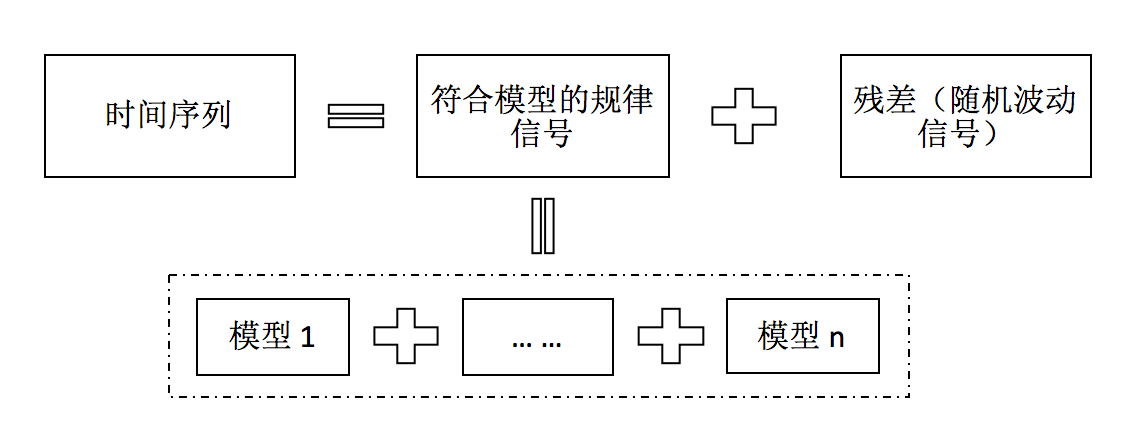
\includegraphics[scale=0.5]{fm-main-structure.png}
\caption{时间序列的可列可加性}
\label{fig:fm-main-structure}
\end{figure}
\begin{figure}[H] 
\centering
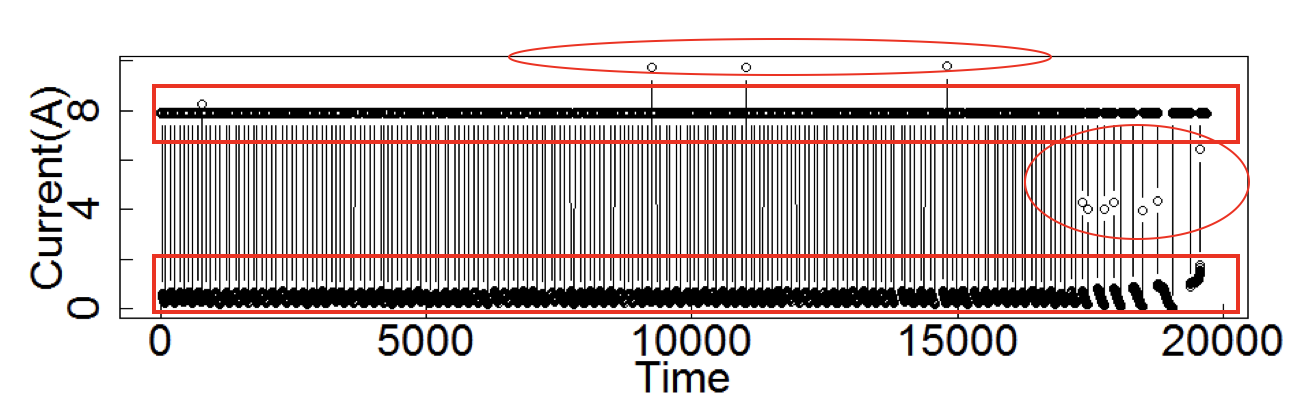
\includegraphics[scale=0.5]{fm-main-example.png}
\caption{来自 NASA IGBT 数据集的电流数据}
\label{fig:fm-main-example}
\end{figure}

(2)随机波动信号萃取:随机波动信号为原生时间序列减去规律信号而得到的残差,反应了系统受各种复杂因素影响的随机波动性,又常称为随机噪音。在异常分析或研究系统对随机波动干扰的抵抗能力时,残差信息尤为关键。 比如图 \ref{fig:fm-main-example} 为 IGBT 系统从正常到失效过程的电流信号,可以看到当系统濒临失效时噪音信号尤为密集(椭圆标出部分)。

在实际分析中明确何时使用何种信号尤为关键。本文在对系统正常情况下的运动轨迹进行建模时关注的是规律信号,参见本文章节\ref{chap:symbolic-regression};而对系统的随机波动性进行研究时,反应系统随机波动性的残差信号是关键,这将是本章的核心资源。



\subsection{系统失效早期预警特征学习}
\label{sec:csd-early-warning-mining}

\subsubsection{系统失效早期预警特征计算}

(1)关键统计量的定义:
\begin{itemize}
  \item 样本均值:定义为\ref{equ:mean},用于估计样本中心,是衡量样本集中程度的指标。
  \item 样本方差:定义为\ref{equ:var},用于估计样本偏离中心的程度,是两个样本离散程度的指标,其值越大说明样本离散程度越高。
  \item 样本协方差:定义为\ref{equ:cov},是衡量两个样本偏差的指标,若两个样本偏离其中心的方向一致则协方差为正,若两个样本偏离其中心的方向不一致则协方差为负,当协方差为零时表示总体无偏差。
  \item 自相关函数:定义为\ref{equ:acf},用于衡量时间序列与其自身滞后\emph{k}步的相关性。
  \item 自回归模型:定义为\ref{equ:ar-model},当前$x_{t}$的值与其前\emph{p}个连续时刻的值相关。$\xi$表示残差。
  \item 偏斜度:定义为\ref{equ:skew},又称样本的三阶中心矩,衡量样本分布的偏斜方向和偏斜程度。当偏斜度为零时说明样本分布以其均值为界具有完美的对称性,然而这在实际中几乎不可能发生;当偏斜度为正时说明样本分布正偏,即相对其均值往右偏离;当偏斜度为负时说明样本分布负偏,即相对其均值往左偏。偏斜度绝对值的大小衡量其偏离的程度,越大偏离程度越显著。
  \item 自相关系数:定义为\ref{equ:lag-1-autocorrelaton}。在对时间序列进行自回归分析时,距离越近相关性越强,因此普遍只通过滞后1个时刻的自相关系数来衡量时间序列与其自身的相关性,其值越大说明相关程度越高。自相关函数和自回归模型的系数都表明时间序列与其自身的相关程度,因此相关性因子可取其一,至于两者之间权衡通常根据实际情况而定。
\end{itemize}

以上的统计指标中样本方差\ref{equ:var},偏斜度\ref{equ:skew},滞后1自相关系数\ref{equ:lag-1-autocorrelaton}是计算早期预警特征的关键统计量。
\begin{subequations}
\begin{align}
& E(x) = \frac{1}{n}\sum_{i=1}^{n}x_{i} , let\ \mu (x)=E(x) \label{equ:mean}\\
& Var(x) = E((x-E(x))^{2}) = \frac{1}{n-1}\sum_{i=1}^{n}(x_{i}-E(x))^{2}, let\ \sigma(x)= \sqrt{Var(x)} \label{equ:var}\\
& Cov(x,y) = E((x-E(x))(y-E(y))) \label{equ:cov}\\
& Acf(x, k) = \frac{Cov(x(t+k), x(t))}{\sigma(x(t+k))\sigma(x(t))} \label{equ:acf} \\
& x_{t} = Ar(x,p) = \alpha_{1}x_{t-1} + \alpha_{2}x_{t-2} + ... + \alpha_{p}x_{t-p} +\xi _{t} \label{equ:ar-model} \\
& Skew(x) = E((\frac{x-\mu(x)}{\sigma(x)})^3) \label{equ:skew} \\[0.1cm]
& Autocorrelation(x) = \left\{\begin{array}{l}
Acf(x, 1)\\ [0.1cm]
\mbox{or}\\[0.1cm]
Ar(x, 1)\\[0.1cm]
\end{array}\right. \label{equ:lag-1-autocorrelaton}
\end{align}
\end{subequations}

% 介绍滑窗的计算方法
(2)以滑窗的形式计算早期预警特征:

首先通过滑窗的形式获取不同时刻对应的固定窗口大小的时间子序列集合。如图\ref{fig:csd-main-sliding-window}所示,坐标轴上每个点对应一个时刻,令滑窗大小\emph{w}为15,自左往右沿着时间轴的方向以1个时刻为步长移动滑窗,每个滑窗对应的连续时间段对应一个子序列。每个滑窗对应的子序列反应了系统在窗口内最后一个时刻的特性。其中滑窗的大小\emph{w}为重要参数,窗口过小有可能引入过多局部细节以至于很难形成对全局临界点的趋势预测指标;而窗口过大有可能掩盖局部重要特征。通过以上操作可以获取子序列集,定义为\ref{equ:rolling-set}。值得注意的是由于窗口大小的限制,前$w-1$个时刻没有对应的子序列,这部分信息将被丢弃,若采样点足够或前期采样点可视为不稳定采样点那么丢弃此部分信息带来的影响可以忽略,但仍需注意窗口设置过大可能导致关键信息丢失的问题。

在获取滑窗时间序列集合后,计算滑动方差\ref{equ:rolling-var},滑动偏斜度\ref{equ:rolling-skew},滑动自相关系数\ref{equ:rolling-autocorrelation}作为早期预警特征。这些基于滑窗计算的特征具有反应系统状态的能力。比如计算滑动方差\ref{equ:rolling-var},$rolling\_var(x)=Var(rolling\_set(x))=\{Var(\{x_{i-w+1,x_{i-w}, ..., x_{i}}\}), ..., Var(\{x_{n-w+1,x_{n-w}, ..., x_{n}}\})\}=\{v_{w}, ..., v_{n}\}$,其中$v_{i}, i=w,w+1,...,n$反应系统在时刻\emph{i}的状态特性。
\begin{subequations}
\begin{align}
& rolling\_set(x) = \{\{x_{i-w+1}, x_{i-w}, ..., x_{i}\} | i=w, w+1, ..., n\} \label{equ:rolling-set} \\[0.1cm]
& rolling\_var(x) = Var(rolling\_set(x)) \label{equ:rolling-var} \\[0.1cm]
& rolling\_skew(x) = Skew(rolling\_set(x)) \label{equ:rolling-skew} \\[0.1cm]
& rolling\_autocorrelation(x) = Autocorrelation(rolling\_set(x)) \label{equ:rolling-autocorrelation}
\end{align}
\end{subequations}

\begin{figure}[H]
\centering
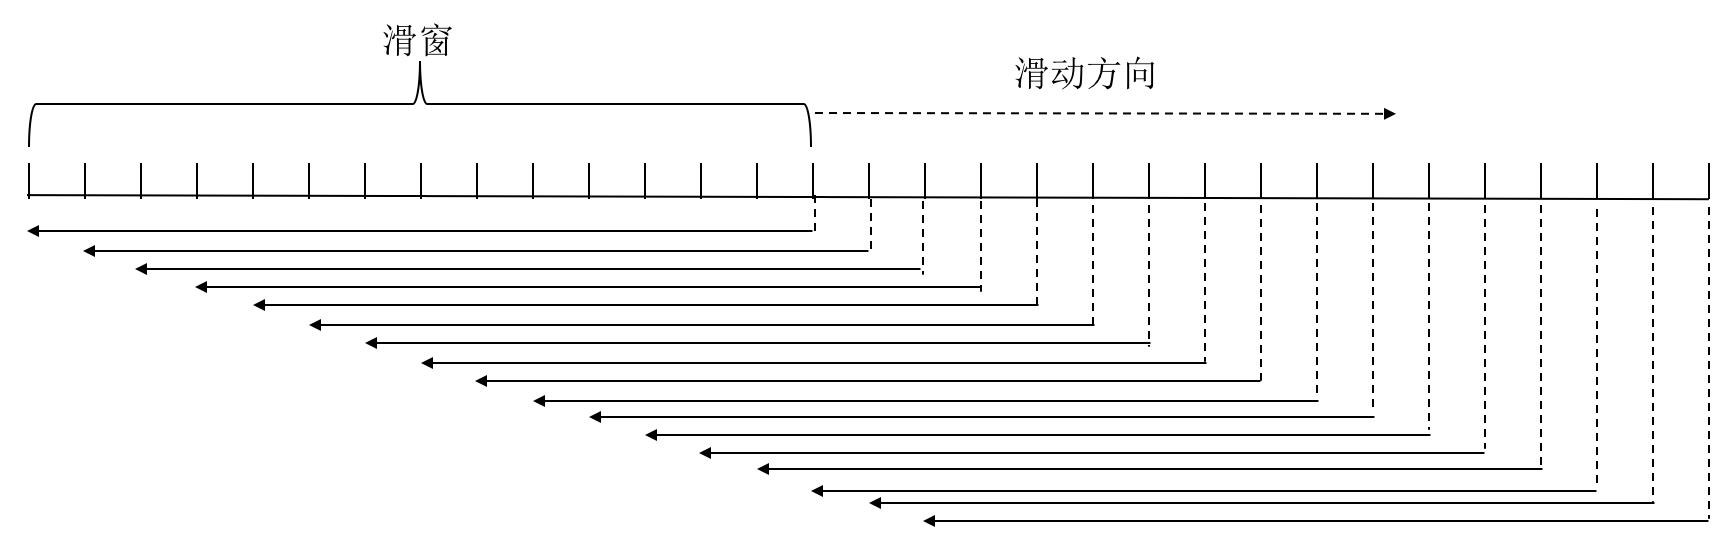
\includegraphics[scale=0.5]{figures/csd-main-sliding-window.png}
\caption{滑窗获取不同时刻时间子序列构成的集合}
\label{fig:csd-main-sliding-window}
\end{figure}

\subsubsection{系统失效早期预警特征显著性检验}

早期预警特征在稳定状态下没有显著波动,当临近系统失效时出现明显的趋势特征,此特征可作为预测指标。本文采用Kendall趋势检验和敏感性分析分别检验早期预警特征的有效性和鲁棒性。

(1)基于Kendall的早期预警特征趋势显著性检验

% 趋势显著性度量
% What is the Mann Kendall Trend Test?: http://www.statisticshowto.com/mann-kendall-trend-test/
% R 的文档“Non-Parametric Trend Tests and Change-Point Detection”,有精确的定义:https://cran.r-project.org/web/packages/trend/vignettes/trend.pdf
% R 的实现文档,更清楚的描述了流程:https://vsp.pnnl.gov/help/vsample/Design_Trend_Mann_Kendall.htm
% 百度百科给出了 Mann Kendall 的优势:https://baike.baidu.com/item/Mann-Kendall%E8%B6%8B%E5%8A%BF%E6%A3%80%E9%AA%8C%E6%B3%95/17829790
Kendall趋势检验为非参数统计检验方法,一般用于检验序列是否存在明显的单调趋势。Kendall趋势检验因具有以下优势得到广泛应用(a)被检验序列无需满足任何先验分布假设,即使存在极端值也可以进行检验;(b)允许被检验序列存在缺失值;(c)检验过程主要分析相对数量级而非数值本身,因此被检验序列可以是微量值;(d)不局限于线性趋势。

Kendall趋势检验的原假设$H_{0}$为“数据来源于相互独立且同分布的总体”,相应的备择假设$H_{A}$为“数据存在单调趋势”。具体检验过程可分为以下几步:

1.计算秩和统计量。通过等式\ref{equ:kendall-s},计算$n(n-1)/2$种可能组合的差并取其符号求和得到\emph{S},其中取符号操作定义为等式\ref{equ:kendall-sgn}。

2.计算\emph{S}的方差。\emph{S}的方差由等式\ref{equ:kendal-sigma}定义,其中\emph{p}表示联结组(由相同数值组成的集合并且元素个数大于1)个数, $t_{j}$ 表示对应的联结组的元素个数。比如对于序列$\{23, 24, 29, 6, 29, 24, 24, 29, 23\}$,联结组个数$p=3$,分别为$\{23, 23\}, \{24, 24, 24\}, \{29, 29, 29\}$并依次从1开始编号,那么可得$t_{1}=2, t_{2}=3, t_{3}=3$。
%值得一提的是\emph{S}的期望为0,即$E(S)=0$。

3.计算趋势度量统计指标。通过\ref{equ:kendall-z-transformation}计算Kendall趋势检验的统计量\emph{Z},正的或负的\emph{Z}值表示序列存在上升或下降的趋势。实践中通常采用由等式\ref{equ:kendall-tau}定义的Kendall's tau 统计量来度量被测序列的趋势,其中\emph{D}定义为\ref{equ:kendall-d}。Kendall's tau 取值区间为[-1,1],当其值为0时表示序列中不存在趋势,否则正数或负数分别表明序列存在上升或下降趋势,其绝对值越大说明趋势越明显。
%本文主要采用 Kendall's tau 作为趋势显著性指标。
\begin{subequations}
\begin{align}
& S = \sum_{k=1}^{n-1} \sum_{j=k+1}^{n} sgn(X_{j} - X_{k}) \label{equ:kendall-s} \\[0.1cm]
& sgn(x) = \left\{\begin{matrix}
 1 & if & x>0 \\ 
 0 & if  & x=0 \\ 
 -1 &  if &{} x<0
\end{matrix}\right. \label{equ:kendall-sgn} \\[0.1cm]
& \sigma^{2} = \frac{n(n-1)(2n+5)-\sum_{j=1}^{p}t_{j}(t_{j}-1)(2t_{j}+5)}{18} \label{equ:kendal-sigma} \\[0.1cm]
& Z = \left\{\begin{matrix}
\frac{S-1}{\sigma} & if  & S>0 \\ 
 0 & if & S = 0\\ 
 \frac{S+1}{\sigma}& if  &  S>0
\end{matrix}\right. \label{equ:kendall-z-transformation}\\[0.1cm]
& \tau = \frac{S}{D} \label{equ:kendall-tau} \\[0.1cm]
& D=[\frac{1}{2}n(n-1)-\frac{1}{2}\sum_{j=1}^{p}t_{j}(t_{j}-1)]^{1/2}[\frac{1}{2}n(n-1)]^{1/2} \label{equ:kendall-d}
\end{align}
\end{subequations}

(2)早期预警特征的敏感性分析
% 之前论文中 method 部分总结的内容。

敏感性分析是检验早期预警特征对不同关键参数的鲁棒性。影响早期预警特征学习结果的关键因素有:随机波动信号挖掘过程采用的时间序列分解方法和滑窗大小。本文对不同参数组合进行大量重复实验,即采用不同窗口大小、不同时间序列分解方法进行早期预警特征学习,并通过Kendall趋势显著性度量各种情况下早期预警特征趋势的显著性,由此观察早期预警特征对参数的敏感性。

\subsection{系统失效与临界相变的一致性检验}
\label{sec:csd-existence-test}

本文基于原生时间序列,通过Wilcoxon符号秩检验、核密度估计、基于AIC的ARIMA分析和动态系统稳定性分析方法进行系统失效与临界相变一致性检验。

(1)Wilcoxon 符号秩检验

由于时间序列通常具有很强的自相关性并且隐含分布不明,因此本文采用非参数统计检验方法Wilcoxon来检验两个样本是否来自同一分布,其判断依据是考察两个样本是否有相同的均值。

假设从系统正常到失效过程采集的时间序列为\emph{x},从序列的正常状态取长度为\emph{w}的子序列$x\_stable = \{x_{i}, x_{i+1}, ..., x_{i+w-1}\}$,并以大小为\emph{w}的滑窗沿失效方向滑动以获取子序列集合$rolling\_set =\{\{x_{j-w+1}, x_{j-w},..., x_{j}\} | j=i+w,...,n\}$。然后检验每个滑窗子序列$x\_rolling \in rolling\_set$是否与$x\_stable$同分布,原假设$H_{0}$为“$x\_stable$和$x\_rolling$来源于同一分布”。

为了作出“接受”或“拒绝”$H_{0}$的决定,本文采用 \emph{p} 值法(又称临界值法)来对假设检验的显著水平进行度量。\emph{p}值是由检验统计量的样本观察值得出的原假设可被拒绝的最小显著性水平。\emph{p}的取值区间为$[0, 1]$,表示拒绝原假设的依据强度,\emph{p}值越小,拒绝原假设的依据越强。一般的,若$p \leqslant 0.01$则称拒绝$H_{0}$的依据很强或称检验是高度显著的;若$0.01 < p \leqslant 0.05$则称拒绝$H_{0}$的依据强或称检验是显著的;$0.05 < p \leqslant 0.1$称拒绝$H_{0}$的理由是弱的,检验不显著;若$p>0.1$一般来说没有理由拒绝$H_{0}$。

每个滑窗子序列$x\_rolling$对应一个\emph{p}值,表示拒绝$H_{0}$的强度,当\emph{p}值小到一定程度时则可有足够依据做出拒绝$H_{0}$的决定,即认为$x\_rolling$和$x\_stable$不同分布,若在系统失效时刻附近\emph{p}值急剧下降到很小的值,则有足够信心拒绝$H_{0}$,即认为此时$x\_rolling$与$x\_stable$不同分布,进而说明系统失效引起了系统状态的急剧改变。

% 核密度估计
(2)核密度估计

在统计领域,核密度估计是一种估计随机变量的概率密度函数的非参数化方法,并且基于高斯核的概率密度估计最为常用。假设从系统正常到失效过程采集的时间序列为\emph{x},将\emph{x}划分为以下3个不相交区间,$x\_stable1=\{x_{i},x_{i+1}...,x_{j}\}$、$x\_stable2=\{x_{k},x_{k+1},...,x_{l}\}$、$x\_failed=\{x_{a},x_{a+1},...,x_{b}\}, 1 \leqslant i,j,k,l,a,b \leqslant n$,分别对应系统的正常状态、正常状态和失效状态。然后通过基于高斯核的概率密度估计方法分别对$x\_stable1, x\_stable2,x\_failed$进行概率密度估计,并对概率密度函数进行可视化比较。若$x\_stable1, x\_stable2$概率密度函数基本一致,而$x\_failed$与前两者有显著不同,这就说明他们所处的状态不同,进而说明系统失效引起了系统状态的转变。

% AIC的ARIMA模型分析
(3)基于AIC的ARIMA模型分析

自相关(AutoRegressive AR)模型定义为\ref{equ:ar},表示当前时刻的观测值$z_{t}$与其自身滞后的\emph{p}个时刻的观察值相关。滑动平均(Moving Average, MA)模型定义为\ref{equ:ma},对于随机游走序列\emph{a},其当前值$a_{t}$可由其相邻的前\emph{p}个时刻的值通过加权平均来估计。自回归滑动平均模型(Autoregressive Moving Average Model, ARMA)定义为\ref{equ:arma},是自相关模型和滑动平均模型的融合。值得注意的是,以上模型的应用需要依赖时间序列稳定性假设,即时间序列中任意两个子序列的联合概率保持不变。但严格意义的稳定性在现实中很难得到满足,因此通常只需要满足弱稳定性假设,即任意子序列的均值和方差保持一致。当弱稳定性假设不能满足时可以通过微分的操作来稳定化原序列,即先通过等式\ref{equ:diff}将原序列进行稳定化后再进行ARMA分析,这通常称为自回归积分滑动平均模型(Autoregressive Integrated Moving Average Model, ARIMA),可表示为$ARIMA(p,d,q)$,$p$表示自相关滞后时长,$d$表示微分阶数,$q$表示滑动平均滞后时长。对于ARIMA模型的评估,有赤池信息量准则(AIC),基于Akaike’s偏差修正的信息准则(Akaike’s bias-corrected information criterion, AICC)和贝叶斯信息准则(Bayesian information criterion, BIC),本文采用AIC。

本文首先通过基于AIC的ARIMA模型对系统失效前的正常状态下对应的时间序列进行拟合学习,由此得到正常状态下的ARIMA模型,然后用此模型来预测未来一个时间段的观测值,预测区间包括失效状态对应的区段。理论上说,如果失效没有引起系统状态转变,正常状态下学习的模型可以对失效状态进行很好的预测,反之则说明失效状态和正常状态不同,进而说明系统失效引起了系统状态的转变。
\begin{subequations}
\begin{align}
& z_{t}=AR(p) = \alpha_{1}z_{t-1} + \alpha_{2}z_{t-2} + ... + \alpha_{p}z_{t-p} + \xi _{t} \label{equ:ar} \\[0.1cm]
& a_{t}=MA(q) = - \theta_{1}a_{t-1} - \theta_{2}a_{t-2} - ... - \theta_{q}a_{t-q} \label{equ:ma}\\[0.1cm]
& y_{t}=ARMA(p, q) =z_{t} + a_{t} = AR(p) + MA(q) \label{equ:arma} \\[0.1cm]
& Diff(d) = z_{t} - z_{t-d} \label{equ:diff} 
\end{align}
\end{subequations}

% 相空间和分叉点分析(Phase-space and Bifurcation analysis)
(4)动态系统的稳定性分析

正常的动态系统具有稳定性,在运行过程中始终向吸引子(Attractor)收敛,即使受到轻微扰动也能很快恢复到稳定状态。如图\ref{fig:csd-early-warning-signal}所示,系统在稳定状态下具有高恢复率,此时盆地的吸引力较大可以抵抗轻微扰动干扰,系统维持在吸引盆中运动;而当系统临近临界相变点时盆地的吸引力变小,相当于吸引盆变浅,此时即使轻微扰动也能将系统推出吸引盆,进而产生急剧的状态变化。

以单变量的时间序列为例,如图\ref{fig:csd-phase-plot-single-variable},纵坐标表示观测序列\emph{x}的一阶微分,反应\emph{x}的运动趋势;横坐标为\emph{x},反应其当前的运动状态。通过解$\frac{dx}{dt}=0$可以得到两个固定点,即图中的点\emph{D}和点\emph{S}。\emph{D}的稳定性分析考察如下:一方面,区间[0,D]的微分为负数,说明\emph{x}在此区间减小,即处于点\emph{D}左下邻域内的运动点有远离\emph{D}的趋势;另一方面,在[D,S]区间内,微分为正,说明\emph{x}在此区间增大,即处于\emph{D}右上邻域内的运动点有远离\emph{D}的趋势;综合两方面,固定点\emph{D}两侧的运动方向背离无法收敛于\emph{D},因此动态系统此时处于不稳定状态。点\emph{S}的稳定性考察如下:一方面,[D,S]区间对应的微分为正,说明\emph{x}在此区间增大,即处于\emph{S}左上邻域内的运动点正在靠近\emph{S};另一方面,[S,inf]对应的微分为负,说明\emph{x}在此区间减小,即处于\emph{S}右下方邻域内的运动点正在靠近\emph{S};综合两方面,固定点\emph{S}邻域的运动都收敛到点\emph{S},即点\emph{S}处于稳定状态。
\begin{figure}[H]
\centering
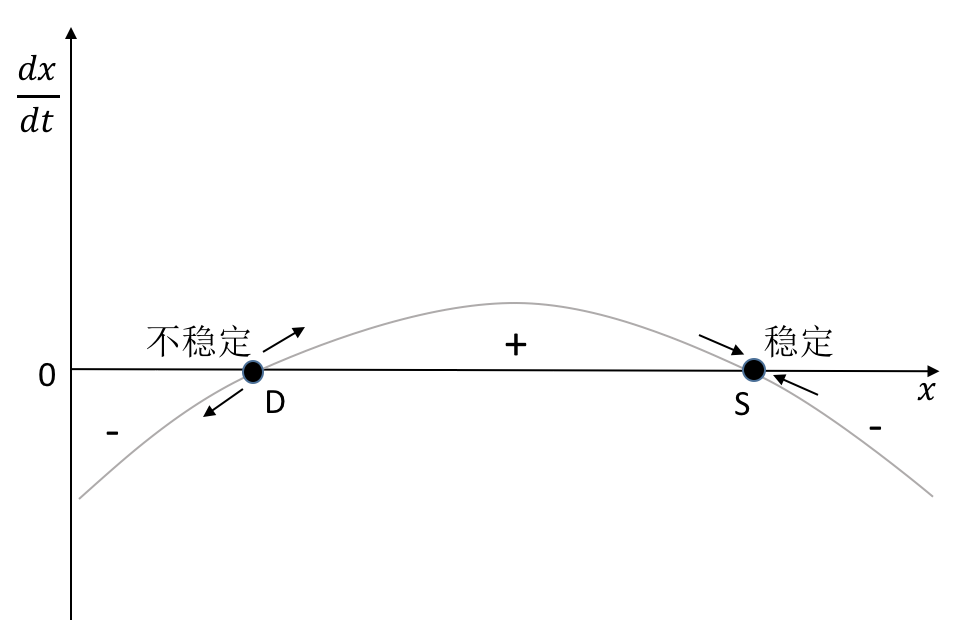
\includegraphics[scale=0.5]{figures/csd-phase-plot-single-variable.png}
\caption{一维离散采样的时间序列相空间图}
\label{fig:csd-phase-plot-single-variable}
\end{figure}
相空间(phase space)分析和分叉点(bifircation)分析常用于动态系统稳定性分析。其中分叉点分析需要知道明确的系统动态方程和分叉因子,难点在于分叉因子依赖很强的领域知识,即使动态方程可以由数据构建也很难在公式中确定分叉因子。因此本文主要采用相空间分析的方法对动态系统的稳定性进行考察。

动态系统可以分为连续型和离散型系统。主要分析流程为,本文首先尝试通过第\ref{chap:symbolic-regression}章介绍的符号回归方法对系统方程(吸引子)或微分方程进行学习。若符号回归方法可以学习有效的系统方程,本文将对应的系统视为连续型系统,并基于系统方程展开稳定性分析。否则,本文将对应的系统视为离散型系统,然后将采集的离散时间序列映射到2或3维、甚至更高维的相空间中以观察动态系统的运动轨迹和状态变化。基于以上分析作出系统是否处于稳定状态的判断。

1. 连续型系统的稳定性分析

根据变量个数的不同进行以下稳定性分析:
\begin{enumerate}[a.]
  \item 单变量模型分析。首先通过符号回归方法学习一维非线性动态方程(微分方程)$\frac{dx}{dt} = f(x)$,然后通过解方程$f(x_{0})=0$得到固定点$x_{0}$,若固定点$x_{0}$满足等式$\frac{\partial f(x)}{\partial x} | x=x_{0} < 0$,则这一点为吸引盆即稳定点。
  \item 多变量模型分析。本文通过符号回归方法学习吸引子的动态性,即多变量之间的关系,基于此本文可以观察系统的运动轨迹。若系统随时间运动过程中维持在吸引子附近,则说明系统的运动是稳定的,其中吸引子的类型有不动点、有限数量的点、有限环、有限环面、奇异吸引子等。若动态系统在运动过程中表现推斥极(repelloer)即向吸引子相反的方向运动,则说明系统处于不稳定状态。
\end{enumerate}
% \begin{subequations}
% \begin{align}
% & \frac{dx}{dt} = f(x) \label{equ:stability-one-dim-dynamic} \\[0.1cm]
% & f(x_{0}) = 0 \label{equ:stability-balance} \\[0.1cm]
% & \frac{\partial f(x)}{\partial x} | x=x_{0} < 0 \label{equ:stability-threshold}
% \end{align}
% \end{subequations}

2. 离散型系统的稳定性分析

离散型系统的状态将满足等式$x_{t+1} = f(x_{t})$,本文不直接对其进行学习,而是基于离散时间序列绘制逻辑斯谛映射图来观察动态系统的轨迹。逻辑斯谛映射图通过绘制 $x_{t+1}$ 对 $x_{t}$ 的二维相空间来反应系统的运动轨迹。以此类推,可以将序列映射到3维甚至更高维的相空间中来观察动态系统更深层的运动规律。最后通过观察系统轨迹是否表现收敛性或吸引子性质来分析当前系统是否处于稳态。
% \begin{equation}
% \label{equ:discrete-ystem}
% x_{t+1} = f(x_{t})
% \end{equation}

\section{系统失效早期预警特征应用}
\label{sec:csd-application}

系统失效早期预警特征直接反映了动态系统随时间变迁的健康状态,可直接通过用户接口进行展示,可以提供给其他机器接口实现状态检测。本节主要介绍针对早期预警特征提出的关键跳变检测算法,由此实现故障预测。

本文以 Wilcoxon 符号秩检验非参数化方法作为关键跳变检测算法设计的基础,主要原因有:(a)早期预警特征在正常状态时保持平稳,当临近系统失效时出现显著趋势,通过假设检验方法可以定位临界点;(b)时间序列分布不明,非参数化方法无需依赖先验分布。
% 介绍假设检验原理,(“临界点”)——「概率论课本180」,可以把书引进来。

核心思想为,在显著水平$\alpha$下,检验假设\ref{csd-ap-hypothesis},其中$H_{0}$为原假设;$H_{1}$为备择假设,假设检验需基于样本作出接受$H_{0}$与$H_{1}$其一的决策。
\begin{equation}
\label{csd-ap-hypothesis}
H_{0}: \mu = \mu_{0}, H_{1}:\mu \neq \mu_{0}
\end{equation}

系统失效早期预警特征在正常状态时保持平稳,因此系统处于正常状态时,早期预警特征的均值保持常数$\mu_{0}$,即接受$H_{0}$;当系统临近失效时,早期预警特征出现偏离正常均值$\mu_{0}$的上升或下降趋势,当偏离足够显著时则可作出拒绝$H_{0}$并接受$H_{1}$的决策,此边界点通常称为{\heiti 临界点},由样本和显著水平$\alpha$同时决定。$\alpha$控制范第I类错误的概率,第I类错误表示假设$H_{0}$实际上为真却被错误的拒绝。

本文有3个指标共同构成系统失效早期预警特征,令长度为$N$的时间序列\emph{x}表示其中任意一个指标。有大小为\emph{W}的滑窗,令$x(1) = \{x_{1}, x_{2}, ..., x_{W}\}$并且其均值为$\mu_{0}$,对应系统初始的稳定状态;以滑窗\emph{W}沿系统失效方向滑动,令$x(i) = \{x_{i-W+1}, x_{i-W}, ..., x_{i}\}, i=W+1,...,N$,其均值为$\mu_{i}$,对应系统在$i$时刻的状态。对$x(1)$和$x(i)$进行Wilcoxon 符号秩检验,并且原假设为$H_{0}: \mu_{0}=\mu_{i}$,$x(1)$表示系统正常状态,若某一时刻在显著水平$\alpha$下$H_{0}$被拒绝,则此刻对应临界点,同时也是预测故障的跳变点。

% reference: 
% https://en.wikipedia.org/wiki/Wilcoxon_signed-rank_test#cite_note-lowry-1
% http://www.r-tutor.com/elementary-statistics/non-parametric-methods/wilcoxon-signed-rank-test
令$xs = x(1), xr=x(i)$,针对单指标变量的 Wilcoxon 符号秩检验的流程如下:
\begin{enumerate}[1.]
  \item 对于$i=1,...,W$,计算$|xs_{i}-xr_{i}|$和$sgn(xs_{i}-xr_{i})$,其中$sgn$表示取符号操作。
  \item 称$(xs_{i}, xr_{i}), i=1,..,W$为一对样本,若$|xs_{i}-xr_{i}|=0$则成对去掉,并令$M$表示剩余样本对数。
  \item 基于$|xs_{i}-xr_{i}|$的大小,对余下的$M$对样本从小到大进行排序。
  \item 获取样本对的秩,即将排序好的样本从1开始进行排名,排名相同的样本对秩为排名均值,令$r_{i}, i=1,...,M$表示样本对$i$的秩。
  \item 计算秩和统计量$R=\sum_{i=1}^{M}[sgn(xs_{i} - xr_{i})*r_{i}]$。
  \item 在原假设,即$H_{0}$假设下,$R$服从均值为0,方差为$\frac{M(M+1)(2M+1)}{6}$的没有表达式的特定分布。若$|R| > R_{C}(\frac{\alpha}{2})$则拒绝原假设,其中$R_{C}(\frac{\alpha}{2})$是临界点。
\end{enumerate}

针对滑动方差、滑动自相关系数、滑动偏斜度3个指标分别执行以上1~5步可以得到各自的秩和统计量,分别表示为$R_{v}, R_{a}, R_{s}$,然后通过等式$U=\frac{R_{v} + R_{a} + R_{s}}{3}$计算融合统计量$U$。同理,在原假设下,$U$服从均值为0的分布,若$|U| > U_{C}(\frac{\alpha}{2})$则拒绝原假设,而第一次使拒绝原假设决策成立的时刻是预测系统失效的跳变点。

\section{实验结果及分析}
\label{sec:csd-experiment}

\subsection{数据集说明}
\label{sec:csd-dataset}	

(1) 机车空气制动器系统数据集

数据集为正在运营的商业机车2016年5月5日到15日的运行数据,数据包括制动管和制动缸的空气压力信号,在此期间空气制动管部分失效。数据通过火车控制和管理系统以1Hz的采样率采集。数据集为列车处于运行状态和停车状态下的观测数据。基于信号与失效相关性分析,本文选用运行时数据作为临界相变早期预警特征学习框架的输入。数据采集环境如图\ref{fig:sr-data-collect}。

(2) 轴承数据集

数据集来源于NASA预测卓越中心的预测数据库\cite{nasa2018}。数据由辛辛那提大学的智能维护系统中心采集,包含三个实验结果集。本文选择第二个实验结果集作为数据源,其中包含从四个轴承中采集的四个传感器信号集。来自轴承1的传感器数据是轴承从正常到失效的振动信号,最后外环失效导致系统停止运行。

(3) 涡扇发动机退化模拟数据集

数据集来源于NASA预测卓越中心的预测数据库\cite{nasa2018}。数据集产生于一个工业增强模拟器C-MAPSS。数据集包含100个仿真单元,每个单元对包含一组独立的测试到失效的过程数据。本文随机选取一组仿真单元数据作为早期预警特征学习的数据源,编号为FD001。这个数据集包含26个信号,为了方便将其表示为V1,V2,...,V26,其中V1是测试单元编号,V2是时间戳,V3-V5是操作配置信号,V6-V26是传感器观测值。在每次试验中,即采集每个单元的测试到失效过程数据时,引擎正常启动并正常运行,然后随机选取一个时刻向系统注入可引起失效的压力以引发系统失效。
%https://www.grc. nasa.gov/WWW/cdtb/software/mapss.html

(4) IGBT加速老化试验数据集

数据集来源于NASA预测卓越中心的预测数据库\cite{nasa2018}。数据集包含来自6个设备的老化数据,其中有一个设备为DC门偏差老化,其余剩下的设备为方信号门偏差老化。本文选择热负荷老化实验采集的子集,实验中通过门电压的DC偏差触发设备老化。感知的信号集包括集电极电流、集电极电压、门电流、门电压、散热器温度和包装温度。在此次加速正常到失效的老化实验中,系统在最后由于闩锁失效。在关闸阶段的集电极电流通常被认为是系统失效的指示信号。本文分析集电极电流、集电极压力和门电流来捕捉信号内和信号间的特性。
% 系统在最后由于闩锁效应(latch-up)失效
% 在关闸(switch-off)阶段

\subsection{实验结果与分析}
% 不同系统中的临界相变早期预警指标
% 说明实验的环境和参数。

实验硬件的主要参数:CPU,Intel(R) Xeon(R) CPU E5-2682,16核,2.50GHz;内存,235GB。所有算法均使用 R3.3.0 实现,若没有特殊说明,所有滑窗计算的窗口大小均为时间序列长度的一半。

(1)系统失效早期预警特征学习的结果展示

针对 4 个不同类型的数据集,分别通过本章\ref{sec:csd-early-warning-mining}描述的早期预警特征学习方法获得滑动方差(Variance)、滑动自相关系数(Autocorrelation(1))和滑动偏斜度(Skewness),并进行显著性和鲁棒性检验。图\ref{fig:csd-early-signal}是机车空气制动器系统数据集、轴承数据集、涡扇发动机退化模拟数据集和IGBT加速老化试验数据集的结果,对应的趋势指标参见表\ref{tab:csd-kd-trend}。结果表明,虽然4类系统差异很大,但临近失效时早期预警特征出现了一致且显著的上升或下降趋势,证明了本文方法的有效性和通用性。

(2)FM框架对早期预警特征的增强效果展示

如图\ref{fig:csd-fm-procedure}所示,本文以IGBT加速老化试验数据集为例展示FM的有效性,具体如下:

1.通过相关性分析发现失效敏感的低工作态信号\emph{x},对应图\ref{fig:csd-fm-procedure}a有颜色圈;

2.通过专家得知\emph{x}正常工作时遵循指数衰减的公式\ref{equ:fit-real-example},进而通过回归方法学习方程的参数,对信号轨迹的拟合效果对应图\ref{fig:csd-fm-procedure}b实线,此部分信号记为\emph{r};

3.计算随机波动信号$s = x - r$,如图\ref{fig:csd-fm-procedure}c所示。

4.基于\emph{s}计算早期预警特征,如图\ref{fig:csd-fm-procedure}f,g,h。

Variance、Autocorrelation(1)、Skewness 三个指标的原趋势分别为0.38、0.86、0.48,参见图\ref{fig:csd-early-signal}和表\ref{tab:csd-kd-trend};经过FM框架处理后的早期特征趋势分别为0.88、0.90、0.88,增强效果显著,充分证明FM框架的有效性。

\begin{figure}[H]
\centering
\begin{subfigure}{\textwidth}
    \centering
    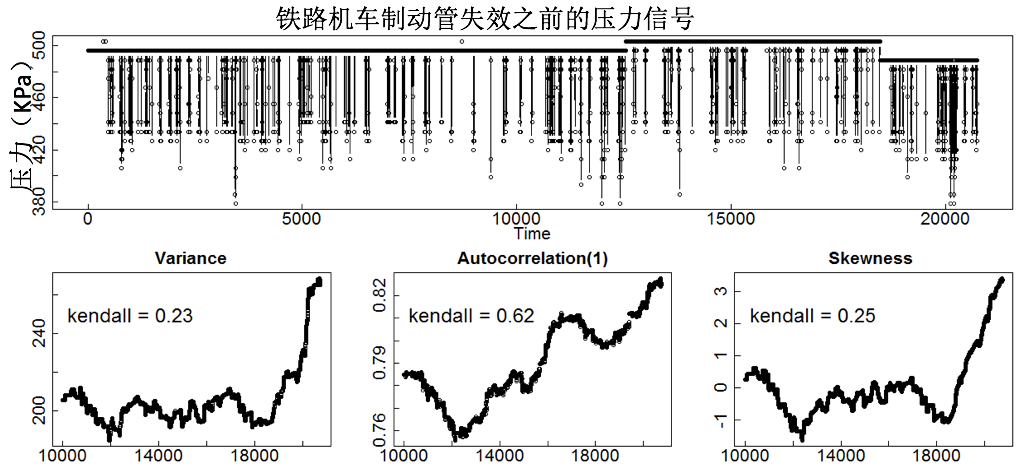
\includegraphics[scale=0.6]{figures/csd/csd-signal-locomotive.png}
\end{subfigure}\\
\begin{subfigure}{\textwidth}
  \centering
  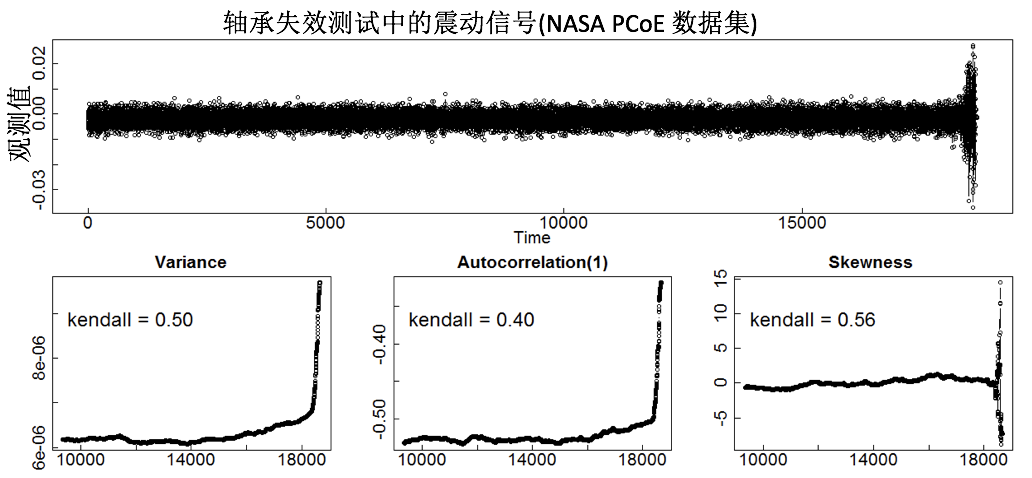
\includegraphics[scale=0.6]{figures/csd/csd-signal-bearing.png}
\end{subfigure}\\
\begin{subfigure}{\textwidth}
    \centering
    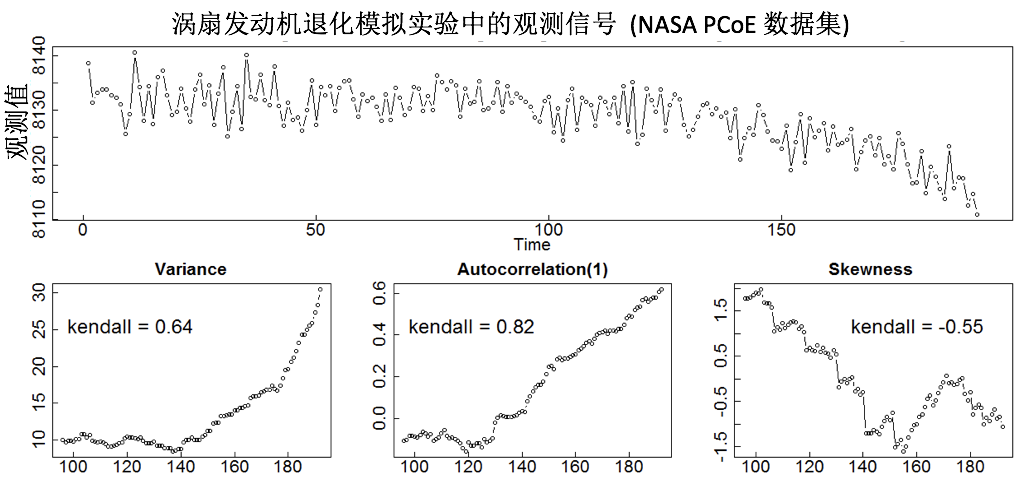
\includegraphics[scale=0.6]{figures/csd/csd-signal-turbofan.png}
\end{subfigure}\\
\begin{subfigure}{\textwidth}
    \centering
    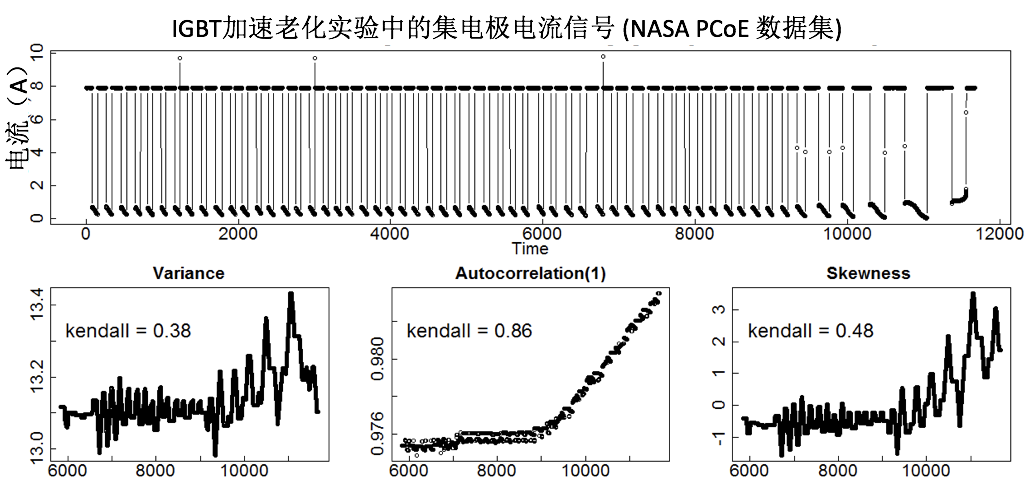
\includegraphics[scale=0.6]{figures/csd/csd-signal-igbt.png}
\end{subfigure}
\caption{基于各系统传感器信号学习的系统失效早期预警特征}
\label{fig:csd-early-signal}
\end{figure}

\begin{table}[htbp]
  \centering
  \caption{各系统早期预警特征的Mann-Kendall趋势指标}
  \label{tab:csd-kd-trend}
    \begin{tabular}{cccc}
      \toprule[1.5pt]
      {\heiti 系统/早期预警特征} & {\heiti Variance} & {\heiti Autocorrelation(1)}  & {\heiti Skewness}\\\midrule[1pt]
      柴油机车制动管 & 0.23 & 0.62 & 0.25 \\
      滚动轴承 & 0.50 & 0.40 & 0.56 \\
      涡轮发动机 & 0.64 & 0.82 & -0.55 \\ 
      IGBT & 0.38 & 0.86 & 0.48 \\
      \bottomrule[1.5pt]
    \end{tabular}
\end{table}

\begin{figure}[H]
\centering
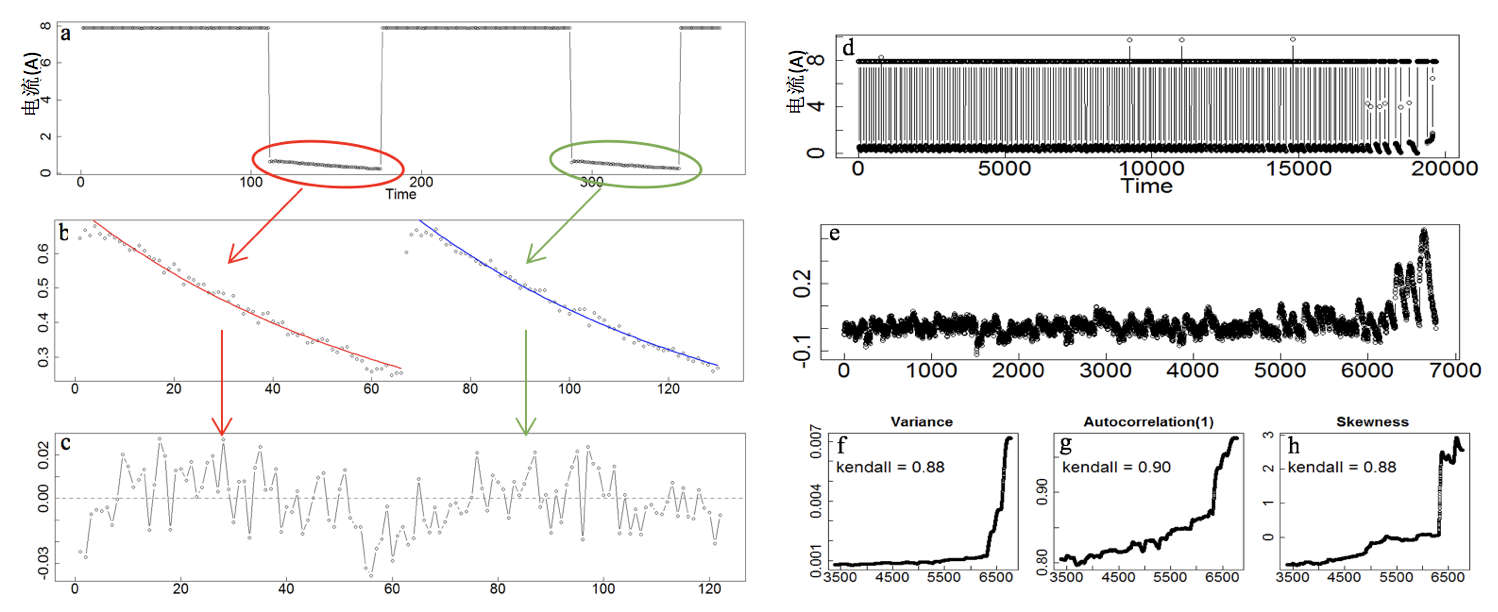
\includegraphics[scale=0.5]{figures/csd/fluctuation-mining.png}
\caption{以IGBT加速老化试验数据集为例的随机波动信号挖掘}
\label{fig:csd-fm-procedure}
\end{figure}

(3) 系统失效与临界相变的一致性检验结果展示

本文通过非参数的Wilcoxon检验方法、核密度估计检验方法、基于AIC的ARIMA模型分析以及动态系统稳定性分析,证明“系统失效引起系统状态转变”,进而将系统失效和临界相变关联起来。具体方法参见本章\ref{sec:csd-existence-test}。

\begin{figure}[H]
\centering
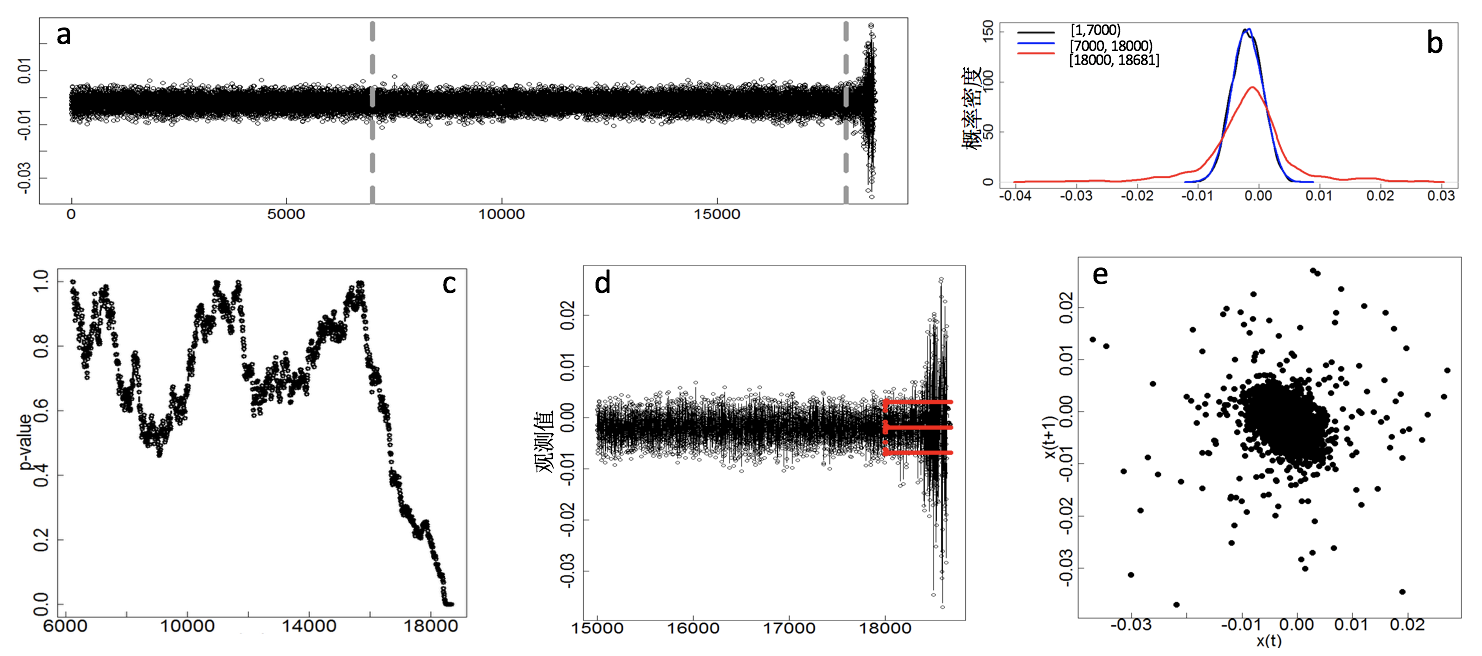
\includegraphics[scale=0.5]{figures/csd/csd-proof-bearing.png}
\caption{轴承系统失效与临界相变一致性检验结果}
\label{fig:csd-proof-bearing}
\end{figure}
针对滚动轴承系统的检验结果,如图\ref{fig:csd-proof-bearing}。\ref{fig:csd-proof-bearing}a 是原生时序震动信号,记为\emph{x},并将其分为不相交的三段,即$s1=x[1,6999], s2=x[7000,17999], s3=x[18000, 18681]$,其中$s1,s2$对应系统正常状态,而$s3$对应系统失效状态。由此展开以下4个方面的验证:

1. 基于高斯核的核密度估计检验结果,如图\ref{fig:csd-proof-bearing}b:$s1,s2$的概率密度趋于一致,而$s3$与前两者显著不同。

2. Wilcoxon检验结果,如图\ref{fig:csd-proof-bearing}c:将代表系统正常状态的$s1$固定,然后以大小为$w=6999$的滑窗从时刻7000开始往系统失效方向滑行,将每次获取的滑窗样本\emph{s}与$s1$进行Wilcoxon检验,并且原假设$H_{0}$为“两个被测样本服从同一分布”。检验结果表明,当滑窗到达时刻15000附近时$p$值急剧下降,当到达系统失效点时,$p$值低于0.01,有很强理由拒绝$H_{0}$,即可断定\emph{s}与$s1$源自不同分布。

3. 基于AIC的ARIMA模型分析的检验结果,如图\ref{fig:csd-proof-bearing}d:首先连接$s1,s2$得到对应系统正常状态的$s=x[1,17999]$,并以此作为训练数据集,基于AIC评估指标学习ARIMA模型;然后利用以上模型对$s3=x[18000, 18681]$进行预测,图示中红色区域是95\%置信度的预测区间;检验结果表明,预测区间可以包含正常状态的样本,但无法包含系统失效时发散的样本。

4. 基于动态系统稳定性分析的检验结果,如图\ref{fig:csd-proof-bearing}e:符号回归方法无法针对振动信号学习系统结构特征,因此采用离散系统下单变量的动态系统稳定性分析方法。首先,将一维振动信号映射到二维相空间以观察其运动轨迹,图中纵坐标为$x(t+1)$,横坐标为$x(t)$,因此图示实际是振动信号的一阶段差分,反映了动态系统的低阶运动轨迹。检验结果表明,$s1,s2$的运动收敛于固定点,而$s3$对应图中发散部分。

以上4个检验结果一致证明滚动轴承系统失效引起系统状态转变。

针对涡扇发动机系统的检验结果,如图\ref{fig:csd-proof}。将样本数据分成两段,$s1=[1,100]$对应系统正常状态,$s2=[101,192]	$对应系统从正常到失效的过程数据。通过符号回归方法学习$s1, s2$的微分方程。结果如\ref{fig:csd-proof}b所示,$s1$对应蓝色,运动方程收敛于固定点;$s2$对应红色曲线,有两个固定点,一个稳定点和一个非稳定点,系统运动具有不稳定性。检验结果证明涡扇发动机系统失效引起系统状态转变。

针对IGBT系统的检验结果,如图\ref{fig:csd-proof}。基于符号回归方法学习系统结构特征,又称吸引子。\ref{fig:csd-proof}c,d对应系统正常状态,系统运动过程中多个信号收敛于有限环。\ref{fig:csd-proof}e,f对应系统失效状态,系统运动过程中没有明显的收敛域。检验结果证明IGBT系统失效引起系统状态转变。


(4)针对早期预警特征的关键跳变检测算法实现故障预测的结果展示

通过本章\ref{sec:csd-application}提出的关键跳变检测算法确定系统失效早期预警特征的跳变点,置信水平$\alpha =0.05$,即置信度为95\%。柴油机车制动管、滚动轴承、涡扇发动机和IGBT的滑窗大小分别为2000,1000,20,1000。结果参见表\ref{tab:csd-alarm-time},早期预警特征的跳变点均早于系统失效时间,对潜在故障具有很好的预测能力。值得注意的是,为便于统一,此处的时刻代表相应数据集的样本编号。
%值得注意的是其中的时刻表示失效点或跳变点在时间序列中对应的下标二非具体的时间,具体的时间可通过采样率算出。比如采油机制动管的采样间隔为1s,分析时按10s进行重采样,早期预警指标比失效时间提前23000-18000=5000,那么实际的时间为10s*5000=50000s=13h,即早期预警指标可以提前13个小时预测到潜在故障。综上,临界相变早期预警指标在工程系统中的应用推广将为普适性的故障预测,PHM架构的部署开辟新的道路。
\begin{table}[htbp]
  \centering
  \caption{系统失效和早期预警特征的跳变时刻对比结果}
  \label{tab:csd-alarm-time}
    \begin{tabular}{ccc}
      \toprule[1.5pt]
      系统 & 失效时刻 &  早期预警特征跳变时刻  \\\midrule[1pt]
      柴油机车制动管 & 20747 & 18660 \\ 
      滚动轴承 & 18681 & 14302 \\
      涡扇发动机 & 192 & 149 \\
      IGBT & 11681 & 9184 \\
      \bottomrule[1.5pt]
    \end{tabular}
\end{table}
% Note: the first 1000 point of Bearing was discarded. 
% 窗口大小:
% 柴油机车制动管:2000
% 滚动轴承:1000
% 涡扇发动机:20
% IGBT:1000
\begin{figure}[H]
\centering
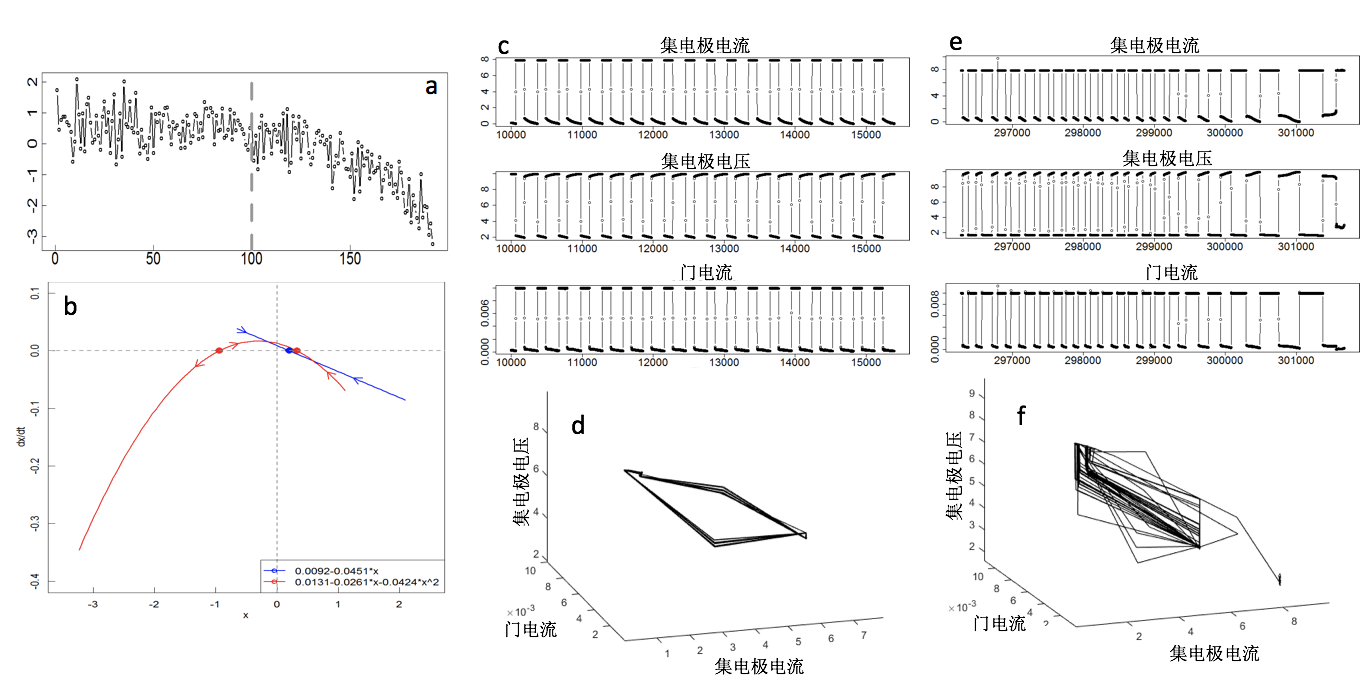
\includegraphics[scale=0.6]{figures/csd/csd-proof.png}
\caption{涡扇发动机和IGBT系统失效与临界相变一致性检验结果}
\label{fig:csd-proof}
\end{figure}

\section{小结}

本章首先对临界相变预测理论以及其与工业系统失效预测的契合点进行了论述;然后将复杂系统临界相变预测理论引入并提出针对工业系统失效预测的早期预警特征学习方法,通过4个不同类型的数据集展开研究。实验结果表明,本文方法可以从差异显著的工业时间序列数据中学习一致且显著的失效早期预警特征;通过多种方法验证了系统失效确实引起系统状态的急剧转变,进一步证明临界相变理论的适用性。最后针对早期预警特征,提出了关键跳变检测算法实现故障预测,实验结果表明早期预警特征跳变时间均显著早于系统失效时间,对潜在故障具有很好的预测能力。

% !TEX root = ../main.tex

\chapter{基于生成式对抗网络的无监督式特征学习与应用}
\label{chap:gan}

\section{引言}

% 时间序列的重要性
神经网络因具有很强的特征学习能力受到广泛关注并取得许多突破进展\cite{lecun2015deep,tsui2015prognostics}。然而现有优秀成果大多为基于判别式模型的监督式学习,正面临着以下挑战:(a)标记数据采集难,比如工业系统的故障、医疗的病变、生态系统的崩溃都是小概率事件。(b)人工标记数据成本高甚至不可行,比如时间序列即使领域专家也很难通过肉眼观察进行区分\cite{langkvist2014review}。(c)判别式模型基于标记数据直接对后验概率进行估计,而非学习数据隐含概率分布,无法反映数据底层特性。

针对以上问题,无监督式学习逐渐成为焦点并在计算机视觉领域取得诸多进展\cite{lee2009convolutional,lecun2015deep,radford2015unsupervised}。生成式模型对数据底层分布进行学习是实现无监督式学习的主要方法,目前最主流的生成式模型有全可视信念网络(FVBN)\cite{frey1998graphical}、变分自编码机(VAE)\cite{russakovsky2015imagenet}和生成式对抗网络(GAN)\cite{goodfellow2014generative}。GAN 因具有计算高效、抗过拟合、学习复杂分布、局限性少等优势倍受关注,并且大量实践表明GAN生成样本的质量更高。目前已有大量研究分别从模型结构\cite{mirza2014conditional,denton2015deep,radford2015unsupervised}、模型理论\cite{chen2016infogan,arjovsky2017wasserstein}和模型应用\cite{isola2017image,ledig2016photo,reed2016generative,salimans2016improved}三个方面对GAN进行优化。

%目前已经有少量针对时间序列数据的无监督式学习方法\cite{langkvist2014review}。
然而GAN的应用目前仍局限于计算机视觉领域,鲜有针对时间序列数据的模型。2018年,Creswell 等人为信号处理领域对GAN的研究进展作了全面综述,但鲜有针对时间序列的成果\cite{creswell2018generative}。针对时间序列数据的研究,截至目前本文只关注到,2017年,Choi 等人的工作\cite{choi2017generating};2017年,Esteban 等人的工作\cite{esteban2017real};2017年,Yahi 等人的工作\cite{yahi2017generative}。然而他们提出的GAN都只针对医疗数据并且只在一个医疗时间序列数据集上进行验证,难以为普遍存在的时间序列提供支持。

% 时间序列分类方法大致可分为两种,即基于距离度量的分类方法和基于特征的分类方法,两类方法效果的优劣直接依赖特征的质量。
时间序列分类是时间序列挖掘的核心任务之一,并且分类优劣直接依赖于特征的质量。基于传统机器学习的分类方法易受模型和数据影响\cite{bagnall2017great}。由于神经网络的优秀表现,逐渐有学者采用深度学习方法解决时间序列分类问题,并且较传统方法的优化效果显著\cite{cui2016multi,wang2017time},充分说明卷积操作对时间序列的处理能力。然而现有成果均为监督式学习方法,在获取足够的标记数据仍面临巨大挑战时难以进行广泛应用。

% 明确本章的工作
针对标记时间序列数据获取难的问题,本章结合生成式对抗网络和卷积神经网络提出时间序列生成式对抗网络(TimeSeris Generative Adversarial Nets, TSGAN),以无监督学习的方式提取有效特征并将其应用于时间序列分类任务。

\section{背景知识}
\subsection{神经网络概述}
\label{tsgan-nn}

\begin{figure}[H]
\centering
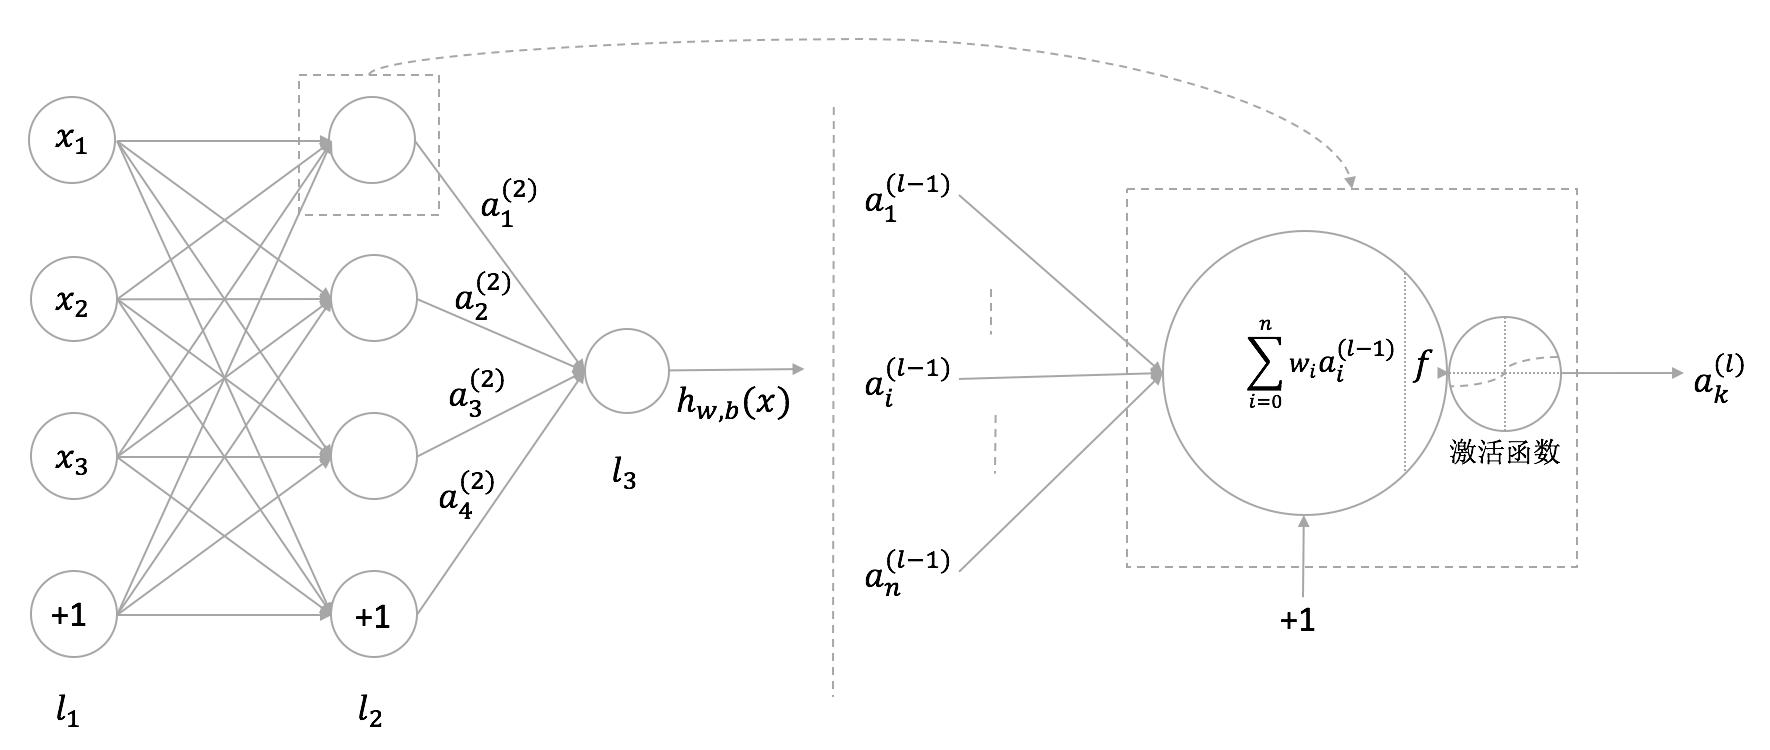
\includegraphics[scale=0.5]{figures/gan-neural-net.png}
\caption{(左)神经网络,(右)神经元}
\label{fig:gan-nn}
\end{figure}

(1)神经网络的基本结构

图\ref{fig:gan-nn}(左)是一个简单的三层神经网络,每一层都由若干个神经元构成。其中第一层为输入层,对应的神经元又称为输入神经元;第二层为隐藏层,对应的神经元称为隐藏神经元;第三层为输出层,对应的神经元称为输出神经元。每个神经元与其前一层所有神经元都有连接,因此这样的神经网络又称为全连接前馈神经网络。更复杂的神经网络无非是由更多隐藏层、更多神经元构成的复杂网络。

图\ref{fig:gan-nn}(右)是神经元结构,神经元负责接收并汇总来自前一层的信息由此作出是否激活的决策。设第$l$层第$k$个神经元的激活信号为$a_{k}^{l}$,其计算过程主要可分为以下两步:(a)汇总信息,假设前一层即第$l-1$层的$n$个神经元传来的信号为$<a_{1}^{l-1},...,a_{i}^{l-1}, ..., a_{n}^{l-1}>$;神经元通过求和得到汇总信息,即$\sum_{i=0}^{n}w_{i}a_{i}^{l-1}$,其中$a_{0}^{l-1}=1$表示神经元对应的偏置,对应图中的+1符号,这样的表示便于进行向量运算和矩阵运算。(b)基于汇总信息作是否激活的决策,即将汇总信息输入激活函数$f$,激活函数根据输入信号强度决定是否向网络下一层单元产生激活信号并计算激活信号强度,直观的激活函数可采用等式\ref{equ:gan-act-func-skip}的阶跃函数实现,只有当信号强度达到某一固定域值$\tau$时神经单元才被激活。综上,一个神经元的运算可归纳为$a_{k}^{l}=f(\sum_{i=0}^{l-1}w_{i}a_{i})$,依次类推可以计算第$l$层所有神经元的输出信号,以及神经网络中所有神经单元的输出信号。

神经网络基于梯度下降算法进行训练,因此神经元的计算必须可导,那么上文介绍的直观阶跃函数\ref{equ:gan-act-func-skip}无法直接作为神经元的激活函数。激活函数可分为线性和非线性两种,由此可对应得到线性神经单元和非线性神经单元。线性激活函数定义为\ref{equ:gan-act-func-identity},一般用在回归问题的神经网络输出层。神经网络逐层叠加神经元,其实相当于简单函数的嵌套叠加,如果其叠加的单元都为线性运算,那么最后得到的复杂表达式化简后还是线性运算,无法具有强大的抽象学习能力。因此神经网络中,尤其是负责特征学习的隐藏单元,基本都由非线性单元构成,嵌套叠加非线性函数形成的复杂函数具备对任何函数的近似能力,进而具有强大的抽象学习能力。其中神经元的非线性由非线性激活函数决定,并且激活函数需具有非线性、连续可倒性和单调性。以下是主流的激活函数:
% Sigmoid激活函数\ref{equ:gan-act-func-sigmoid},Tanh激活函数\ref{equ:gan-act-func-tanh},ReLU激活函数\ref{equ:gan-act-func-relu},PReLU激活函数\ref{equ:gan-act-func-parametric-relu}
\begin{itemize}
  \item Sigmoid 激活函数,又称 Logistic 函数,定义为\ref{equ:gan-act-func-sigmoid}。Sigmoid 最大的特点是其输出区间为[0,1],和概率的区间一致,因此可以天然的表达样本出现的可能性,通常用于二分类问题的神经网络的最后一层,对于多分类问题通常使用Softmax函数。然而 Sigmoid 函数具有以下不足:(a)存在梯度消失问题,当神经网络逐渐加深时,梯度的强度将变得很微弱甚至可忽略不计,由此基于梯度的训练过程将停止;(b)输出区间没有以0为中心,这将导致梯度更新因方向不同具有很大差距,并且这样的不对称性会使优化过程更困难;(c)Sigmoid 对于很大或很小的输入会出梯度饱和现象;(d)Sigmoid 收敛速度慢。
  % 一般只用于输出层
  \item Tanh 激活函数,定义为\ref{equ:gan-act-func-tanh}。针对 Sigmoid 不以0为中心对称的问题,Tanh 对 Sigmoid 的输出进行变换,实际上$Tanh(x) = 2sigmoid(2x)-1$,由此可得到[-1,1]区间上的对称输出,使训练优化过程更容易。因为Tanh 激活函数是 Sigmoid 函数的变形,因此仍然存在梯度消失和梯度饱和的问题。
  % 一般只用于输出层
  \item ReLU 激活函数,定义为\ref{equ:gan-act-func-relu}。ReLU 解决了梯度消失问题并且收敛速度快,因此在深度学习中得到广泛应用,但值得注意的是ReLU只能用于神经网络的隐藏单元。ReLU的不足之处在于,当输入信号为负数时对应的函数值全为0,这可能会导致死神经元(Dead Neurons)问题,即有些神经元会在训练过程中停止更新。
  %ReLU收敛速度快,近期已有研究证明ReLU激活函数的收敛效率是Sigmoid和Tanh的6倍。
  \item LeakyReLU、ParametricReLU和RandomizedReLU激活函数,解决了ReLU激活函中存在的死神经元问题。ParametricReLU 的定义为\ref{equ:gan-act-func-parametric-relu},特殊的当$\alpha = 0.01$时为LeakyReLU,训练时若通过随机算法在$\alpha$取值范围内随机确定参数,则称为RandomizedReLU。
\end{itemize}

对于激活函数的选择很难有确切的定论,目前 Sigmoid 和 Tanh 激活函数已很少用于神经网络的隐藏单元,通常根据问题的需要用于输出单元。当下的神经网络,尤其是卷积神经网络和深度神经网络的隐藏单元基本都选用ReLU函数和基于此的改进,比如LeakyReLU,ParametricReLU和RandomizedReLU。
% 激活函数的 reference
% !!对激活函数的优缺点和发展介绍得比较清晰:https://towardsdatascience.com/activation-functions-and-its-types-which-is-better-a9a5310cc8f
% 简单概括,其中的表格和wiki的类似:https://towardsdatascience.com/activation-functions-neural-networks-1cbd9f8d91d6
% wiki,有一个很全的表格:https://en.wikipedia.org/wiki/Activation_function
% 最开始看到的,但废话还是比较多,不好:https://medium.com/the-theory-of-everything/understanding-activation-functions-in-neural-networks-9491262884e0
% tf activation function: tf.nn.relu, tf.nn.relu6, tf.nn.crelu, tf.nn.elu, tf.nn.selu, tf.nn.softplus, tf.nn.softsign, tf.nn.dropout, tf.nn.bias_add, tf.sigmoid,tf.tanh
\begin{subequations}
\begin{align}
a = f(x) &= Skip(x) = \left\{\begin{matrix}
1 & x \geqslant \tau  \\ 
0 &  x < \tau  
\end{matrix}\right. , a \in \{0, 1\} \label{equ:gan-act-func-skip} \\
a = f(x) &= Linear(x)=x , a \in (-\infty, \infty) \label{equ:gan-act-func-identity}\\
a = f(x) &= Sigmoid(x) = \frac{1}{1+e^{-x}} \label{equ:gan-act-func-sigmoid}, a \in [0, 1] \\
a = f(x) &= Tanh(x) = \frac{1}{1+e^{-2x}} - 1 \label{equ:gan-act-func-tanh} , a \in [-1, 1] \\
a = f(x) &= ReLU(x) = \left\{\begin{matrix}
x & x \geqslant 0 \\ 
0 &  x < 0
\end{matrix}\right. , a \in [0, \infty) \label{equ:gan-act-func-relu}\\
a = f(x) &= PReLU(x) = \left\{\begin{matrix}
x & x \geqslant 0 \\ 
\alpha x &  x < 0, abs(\alpha) \leq 1
\end{matrix}\right. , a \in (-\infty, \infty) \label{equ:gan-act-func-parametric-relu}
\end{align}
\end{subequations}

(2)神经网络的训练

设有$m$个样本的训练集$\{(x^{(1)}, y^{(1)}), ..., (x^{(i)}, y^{(i)}), ..., (x^{(m)}, y^{(m)})\}$。令$W_{i,j}^{l}$ 表示第\emph{l}层的第\emph{j}个神经元到第$l+1$层的第\emph{i}个神经元的权重;$z_{i}^{l}$表示第\emph{l}层第\emph{i}个神经元的求和结果;$a_{i}^{l}$表示第\emph{l}层的第\emph{i} 个神经元的输出,具体的对于输入层$a_{i}^{1} = x_{i}$,对于隐藏层$a_{i}^{l}$为激活函数的计算结果,特殊的$a_{0}^{l}$表示偏置,对应权重为$W_{i,0}^{l}$。

设神经网络最后的输出为$h_{W}(x)$,易知$ h_{W}(x) = a^{l}$。由此可得单个样本输入$(x,y)$的损失函数定义为等式\ref{eq:gan-nn-cost-func},实际上是估计值和真实值之间的均方误差。对于整个数据集的损失函数为等式\ref{eq:gan-nn-loss-func},其中$n_{l}$表示神经网络的层数,$s_{l}$表示第\emph{l}层的神经元个数。等式\ref{eq:gan-nn-loss-func}由两部分组成,第一部分为所有样本的均方误差,第二部分为正则化项,定义采用的是$L_{2}$正则,$\lambda$为正则项的权重,值得注意的是偏置项不惩罚。
\begin{equation}
\label{eq:gan-nn-cost-func}
J(W;x,y) = \frac{1}{2}\left \| h_{W}(x) - y \right \|^{2}
\end{equation}
\begin{equation}
\label{eq:gan-nn-loss-func}
J(W) = [\frac{1}{m}\sum_{i=1}^{m}J(W;x^{(i)}, y^{(i)})] + \frac{\lambda}{2}\sum_{l=1}^{n_{l}-1}\sum_{i=1}^{s_{l}}\sum_{j=1}^{s_{l-1}}(W_{i,j}^{l})^{2}
\end{equation}

神经网络优化的目标是最小化损失函数,而梯度是函数上升最快的方向,那么梯度的反方向就是函数下降最快的方向,因此神经网络采用梯度下降的寻优方法获取最优解。其核心思想为,从某一初始值开始,每次都找到当前梯度最大的方向,然后沿这一方向的反方向对函数的各参数进行更新,即通过等式\ref{equ:gan-nn-update}对权重进行更新,其中$\alpha$为学习率。
\begin{equation}
\label{equ:gan-nn-update}
W_{i,j}^{l} = W_{i,j}^{l} - \alpha \frac{\partial J(W)}{\partial W_{i,j}^{l}} 
\end{equation}

神经网络的训练过程为,对于每个输入样本(x,y)重复进行以下操作:
% 【梯度下降,随机梯度下降?区别是否要说?】
\begin{enumerate}[1.]
  \item 基于前向传播的方式计算神经网络每个神经元的输出,即依次对$2,3,..,n_{l}$层网络的各个神经元进行如下计算
  \begin{enumerate}
    \item $z_{i}^{l} = \sum_{j=0}^{n}W_{i,j}^{l-1}a_{j}^{l-1}, a_{0}^{l-1}=1$
    \item $a_{i}^{l} = f(z_{i}^{l})$
  \end{enumerate}
  \item 计算神经网络最后一层(第$n_{l}$层)的各个神经元对误差的反馈因子:

  $\delta_{i}^{n_{l}} = \frac{\partial \frac{1}{2} \left \| y - h_{W}(x) \right \|^{2}}{\partial z_{i}^{n_{l}}} = -(y_{i}-a_{i}^{n_{l}} )f'(z_{i}^{n_{l}})$

  \item 基于后向传播的方式计算神经网络每个神经元的误差反馈因子,即依次对$l$($l=n_{l}-1, n_{l}-2, ..., 2$)层的神经单元 进行以下计算:

  $\delta_{i}^{l} =(\sum_{j=1}^{s_{l+1}}W_{j,i}\delta_{j}^{l+1})f'(z_{i}^{l})$

  \item 同时对网络各个节点的权重进行更新:

  $W_{i,j}^{l} = W_{i,j}^{l}- \bigtriangledown W_{i,j}^{l}, \bigtriangledown W_{i,j}^{l} = \frac{\partial J(W;x,y)}{\partial W_{i,j}^{l}} = a_{j}^{l}\delta_{i}^{l+1}$

\end{enumerate}

\subsection{卷积神经网络概述}
\label{tsgan-cnn}
% reference: 
% http://cs231n.github.io/convolutional-networks/
% https://ujjwalkarn.me/2016/08/11/intuitive-explanation-convnets/

\begin{figure}[H]
\centering
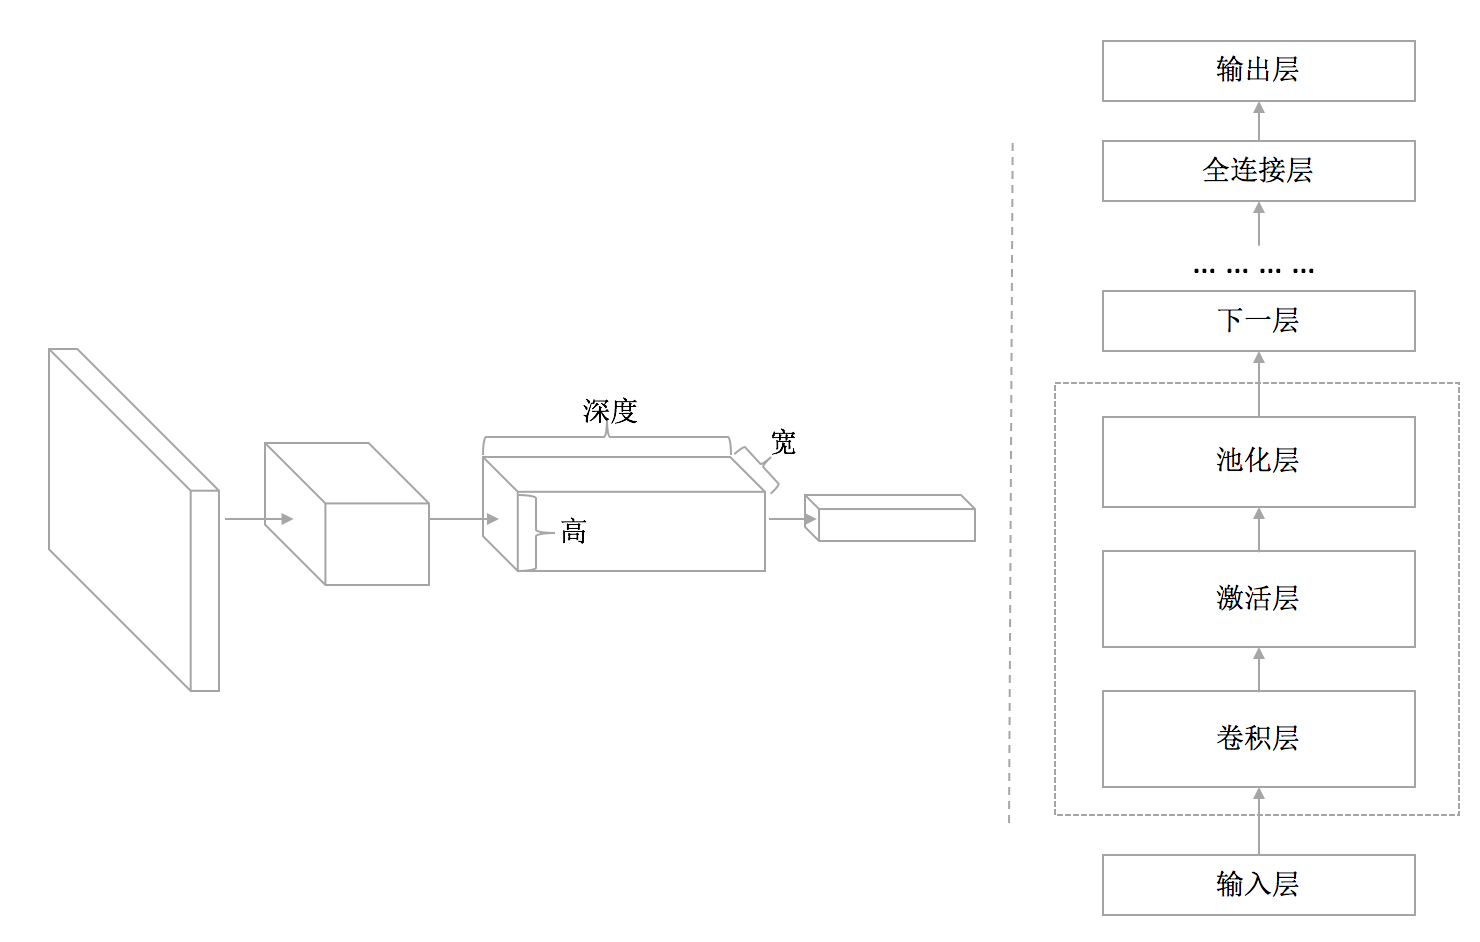
\includegraphics[scale=0.5]{figures/gan-cnn.png}
\caption{(左)卷积神经网络,(右)卷积神经网络的基本组织结构}
\label{fig:gan-cnn}
\end{figure}

图\ref{fig:gan-cnn}(左)是一个简单的4层卷积神经网络。卷积神经网的运算对象均表示为3维矩阵,令$[w, h, c]$表示宽为$w$,高为$h$,深为$c$的矩阵。比如一张像素为24*24的RGB彩色图片,可表示为[24, 24, 3],深度3表示RBG三色通道。

图\ref{fig:gan-cnn}(右)是卷积神经网络的基本结构。一次完整的卷积运算一般由卷积层(Convolutional Layer)、激活层(Active Layer)和池化层(Pooling Layer)叠加的基本单元完成(对应图中虚线框),更深的卷积神经网络是以上基本单元的叠加结果。卷积层实现提取局部特征的矩阵运算,激活层是激活函数非线性单元,池化层负责降采样。另外,全连接层(Fully Connected Layer)一般对应一个浅层全连接前馈神经网络,负责连接各局部特征,由此得到特征向量支持输出层完成分类、预测等机器学习任务。

(1)卷积层

卷积层进行卷积运算。以二维矩阵为例,如图\ref{fig:gan-cnn-ops},输入为3*4的矩阵$X$,卷积核$K$为2*2的矩阵。卷积运算为,以与$K$相同规模的矩阵为滑窗,从$X$的左上方开始,从左至右,从上至下滑动,每次从$X$截取窗口大小的区块$W$,这样的区块通常称为感知域(reception filed),然后计算$W$和$K$的点积(两个矩阵对应位置相乘再求和)。图\ref{fig:gan-cnn-ops}红色矩形对应第一次卷积运算,依此类推,以1为步长,从左至右,从上至下滑动窗口完成余下所有计算,最后得到一个二维矩阵,通常称为特征映射(Feature map)。此过程可形式化的定义为等式\ref{eq:gan-cnn-conv},$m,n$分别表示窗口的宽和高,$Z$为输出矩阵,$Z_{i,j}$表示$Z$在第$i$行,第$j$列的元素。

一般化到三维输入,令$X=[w, h, c]$表示宽为$w$,高为$h$,深为$c$的矩阵输入,对应的卷积核也是三维矩阵并且深度必须和输入的深度一致,表示为$K=[m, n, c]$。卷积运算过程为,以同$K$规模一样的窗口,并令步长为1,在$X$上进行滑窗计算,形式化的定义为等式\ref{eq:gan-cnn-conv-3d}。值得注意的是输出为二维矩阵。
\begin{equation}
\label{eq:gan-cnn-conv}
Z_{i,j} = (X*K)(i,j) = \sum_{m}\sum_{n}X_{i+m, j+n}K_{m,n}
\end{equation}
\begin{equation}
\label{eq:gan-cnn-conv-3d}
Z_{i,j} = (X*K)(i,j) = \sum_{m}\sum_{n}\sum_{d}X_{i+m, j+n,d}K_{m,n,d}
\end{equation}

卷积运算涉及的卷积核是需要学习的参数并且一次完整的卷积运算共享一个卷积核,因此卷积运算具有参数共享的性质,由此相比于全连接前馈网络大大减少了所需学习的参数量,进而更省空间。一次卷积运算需要一个卷积核,一个卷积核对应一个二维矩阵输出,通常一次这样的运算只能提取一种或一类特征。因此需要若干相同规模的卷积核进行多次卷积运算以得到多个对应不同类型特征的二维矩阵,最后将这些矩阵拼接可得到三维特征矩阵。

令$Z=[w_{z}, h_{z}, c_{z}]$表示输出的三维特征矩阵,其规模由卷积核个数、卷积核规模和滑窗运算步长(stride)共同决定。令$X=[w_{x}, h_{x}, c_{x}]$表示输入,$n_{f}$表示卷积核个数,$K=[w_{k},h_{k},c_{k}]$表示卷积核,$s$表示步长,那么$w_{z} = \left \lfloor (w_{x} - w_{k})/s \right \rfloor + 1, h_{z} = \left \lfloor (h_{x} - w_{k})/s \right \rfloor + 1, c_{z} = n_{f}$。

可以注意到除非$w_{k}=h_{k}=1$且$s=1$,否则输出规模必然小于输入规模。因此对于多层卷积神经网络,逐层进行以上卷积运算,特征矩阵很快就会缩小到无法计算的程度(当特征矩阵比卷积核还小时,无法继续进行运算)。如图\ref{fig:gan-cnn-padding}(左),以一维向量运算为例,卷积核大小为3,步长为1,特征向量从5个元素减少到3个元素,以此递减元素个数将很快减小到1。为了构建深度卷积神经网络,通常需要卷积操作的输出规模不要减小或减小得不那么急剧,由此引入了一个重要操作,即零填补(zero-padding),通常称为填补(padding)。padding在卷积运算前使用0来填充输入矩阵的边沿由此降低输出规模减小的速度。假设零填补参数为$p$,此时 $w_{z} = \left \lfloor (w_{x}+2p-w_{k})/s \right \rfloor + 1, h_{z} = \left \lfloor (h_{x}+2p-h_{k})/s \right \rfloor+1$。如图\ref{fig:gan-cnn-padding}(右),以一维向量运算为例,卷积核大小为3,步长为1,零填补参数为1(白色圈对应填补),由此保证输出规模与输入相同,进而支持多次类似运算得以实现。

通常卷积操作根据有无填补分为两种模式:(1)不使用填补操作,对应图\ref{fig:gan-cnn-padding}(左);(2)设置适当的填补参数$p$使得输出规模和输入规模相同,对应图\ref{fig:gan-cnn-padding}(右)。
% padding 有两种方式,一般称为same,valid。

\begin{figure}[H]
\centering
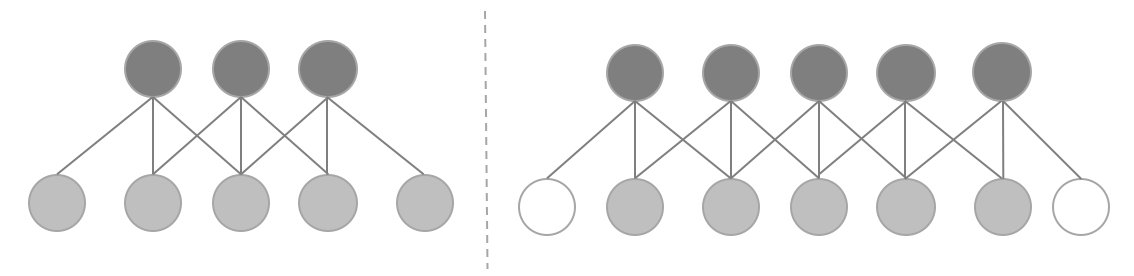
\includegraphics[scale=0.5]{figures/gan-cnn-padding.png}
\caption{(左)无填补的运算结果;(右)填补参数为1的运算结果}
\label{fig:gan-cnn-padding}
\end{figure}

(2) 激活层

激活层是使卷积神经网络具有非线性的关键,由激活函数构成,在卷积神经网络中通常使用ReLU激活函数及其变种,Sigmoid和Tanh只在输出层使用。如图\ref{fig:gan-cnn-ops},激活层对卷积层输出的特征矩阵的每一个元素进行激活运算,并将计算结果输入到池化层。对激活函数介绍参见\ref{tsgan-nn}。

(3) 池化层

池化层主要的作用是降采样,同时池化操作可以让卷积神经网络具有不变式(invariant)特性。池化层运算的核心思想为,通过给定的滑窗进行规约运算,即用一个统计值表示滑窗对应的区块,进而实现降维的目的。如图\ref{fig:gan-cnn-ops},以2*2的滑窗进行池化运算为例,图中蓝色框对应第一次运算,使用窗口对应区块内的最大值表示当前区块,依次从左往右、从上往下、以步长为1的方式滑动窗口并重复以上运算,此过程通常称为最大池化(max pooling),常用的还有均值池化(average pooling)。一般的,假设输入$X=[w_{x}, h_{x}, c_{x}]$,滑窗规模为$[w_{p}, h_{p}]$,滑动步长为$s$,那么对于输出$Z=[w_{z}, h_{z}, c_{z}]$,$w_{z} = \left \lfloor (w_{x}-w_{p})/s \right \rfloor+1, h_{z} = \left \lfloor (h_{x}-h_{p})/s \right \rfloor+1, c_{z}=c_{x}$。

(4)全连接层

 全连接层在卷积神经网络的最后一层,是浅层(通常是一层),全连接前馈网络,由此实现比如分类或回归等机器学习任务。在此之前,通常需要进行压平(flatten)操作将三维矩阵转换成向量的形式。

\begin{figure}[H]
\centering
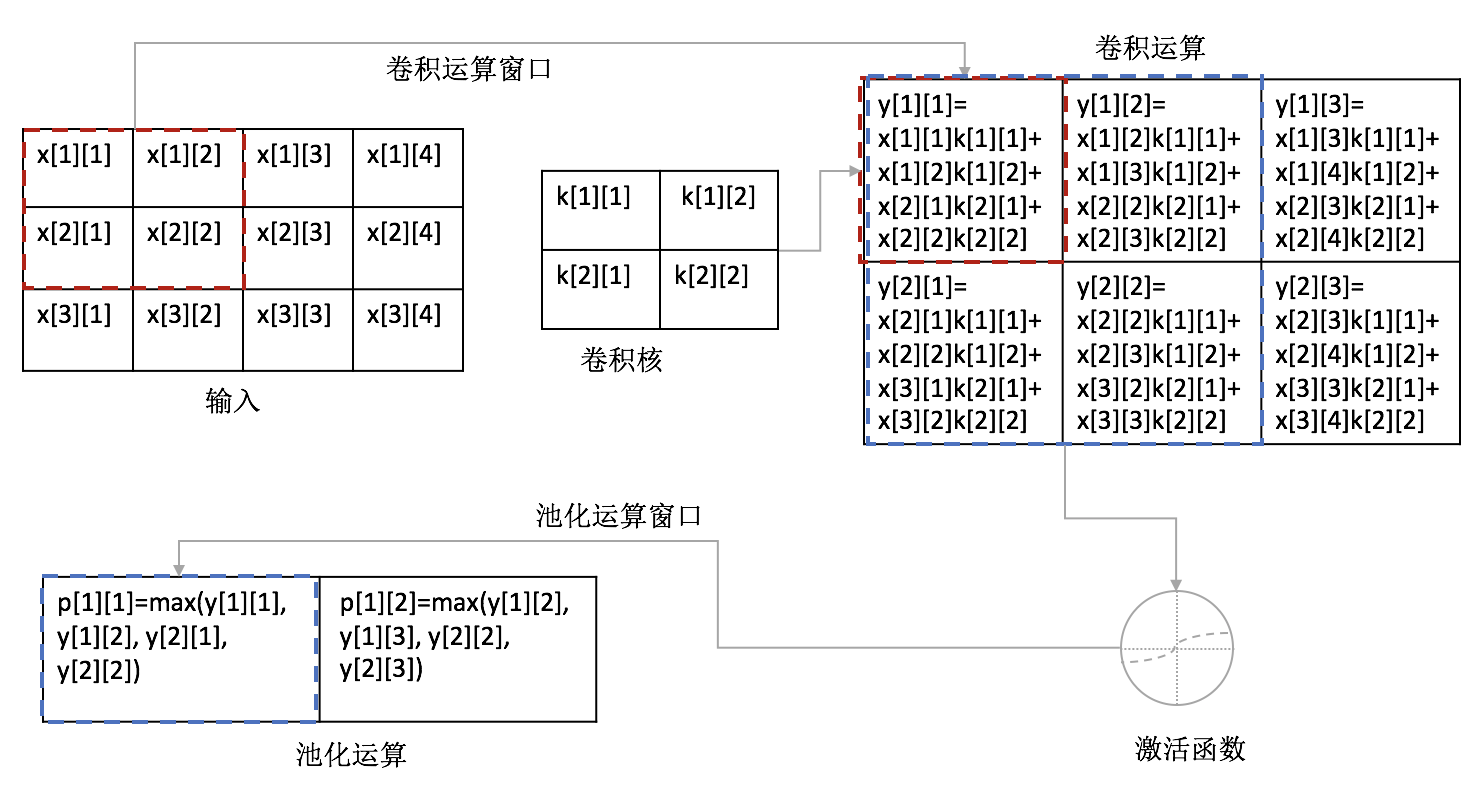
\includegraphics[scale=0.5]{figures/gan-cnn-ops.png}
\caption{卷积神经网络的一次卷积、激活和池化运算}
\label{fig:gan-cnn-ops}
\end{figure}

\section{无监督式时间序列特征学习}
\label{tsgan-model}
% DCGAN:
% Replace any pooling layers with strided convolutions (discriminator) and fractional-strided convolutions (generator).
% Remove fully connected hidden layers for deeper architectures.
% Remove fully connected hidden layers for deeper architectures.
% Use ReLU activation in generator for all layers except for the output, which uses Tanh.
% Use LeakyReLU activation in the discriminator for all layers.
%
% Different Convolution operation
% 中文,介绍得还挺清楚:https://buptldy.github.io/2016/10/29/2016-10-29-deconv/
% An Introduction to different Types of Convolutions in Deep Learning: https://towardsdatascience.com/types-of-convolutions-in-deep-learning-717013397f4d
% Theano 的 tutorial, 似乎更详细:http://deeplearning.net/software/theano/tutorial/conv_arithmetic.html
%
% Batchnorm
% 原文【把原文batch-norm操作的算法copy过来就可以,说明优势】:https://arxiv.org/abs/1502.03167

针对标记时间序列数据获取难的问题,本文提出时间序列生成式对抗网络(TSGAN)。TSGAN的生成器是一个卷积神经网络,负责学习真实时间序列数据集的分布,如图\ref{fig:gan-ts-generator},基于噪音输入生成时间序列样本;TSGAN的判别器是由卷积神经网络构成的二分类器,如图\ref{fig:gan-ts-discriminator},其输出为样本确实来自真实数据集的概率;TSGAN 通过生成器和判别器相互博弈进行训练,算法\ref{gan-tsgan-algorithm},基于梯度下降和反向传播算法进行迭代更新。生成器以生成更真实的时间序列样本为目标,即最大化其生成样本在判别器中的输出概率;判别器以正确辨别样本真伪为目标,即最大化真实样本的输出概率的同时最小化生成样本的输出概率。

(1)TSGAN的基本运算

TSGAN的核心由两个卷积神经网络构成,有关神经网络的介绍见本章\ref{tsgan-nn},卷积神经网络参见本章\ref{tsgan-cnn}。这里主要介绍两个特殊运算,即小数跨步卷积(Fractional Strided Convolution, FSC)\cite{dosovitskiy2015learning}和批量归一化(Batch Normalization)\cite{ioffe2015batch}。

1. 小数跨步卷积

%Convolution: Convolution+Pooling; Deconvolution: Unpooling+Convolution。
小数跨步卷积,又可称转置卷积(Transpose Convolution)或反卷积(Deconvolution)。一般,卷积神经网络的运算顺序为先进行卷积运算然后进行池化运算;而小数跨步卷积可看成以上运算的逆过程,先进行反池化运算然后进行卷积运算。

反池化运算的核心思想是:令各维度的步长为$s$,输入$X=[w_{x}, h_{x}, c_{x}]$,输出$Z=[w_{z}, h_{z}, c_{z}]$。首先将$X$的每个元素映射为$s*s$规模的区块并将该元素放置于区块左上方,同时区块其他位置补0;由此可以得到$w_{x}*h_{x}$个规模为$s*s$的区块,拼接以上区块得到输出$Z$,容易得$w_{z}=w_{x}*s, h_{z} = h_{x}*s, c_{z}=c_{x}$,输出规模相比于输入规模扩大了$s$倍。

池化的作用是降维,而反池化的作用是升维。如图\ref{fig:gan-unpooling}通过反池化操作实现对输入的两倍扩大。如图\ref{fig:gan-unpooling}(上),$s=2$,输入为$X=[2, 2, c_{x}]$,经过反池化操作后得到输出$Z=[4, 4, c_{z}]$,规模扩大2倍;如图\ref{fig:gan-unpooling}(下),$s=2$,输入为$X=[3, 3, c_{x}]$,经过反池化操作后得到输出$Z=[6, 6, c_{z}]$,规模扩大了2倍。

综上所述,小数跨步卷积先进行反池化运算然后进行卷积运算,对于步长$s$,相当于扩大输入$s$倍并且完成局部特征提取。
%经过 unpooling 以后使用same模式的convolution就可以实现每次增加两倍的目标。以上操作称为deconv。

\begin{figure}[H]
\centering
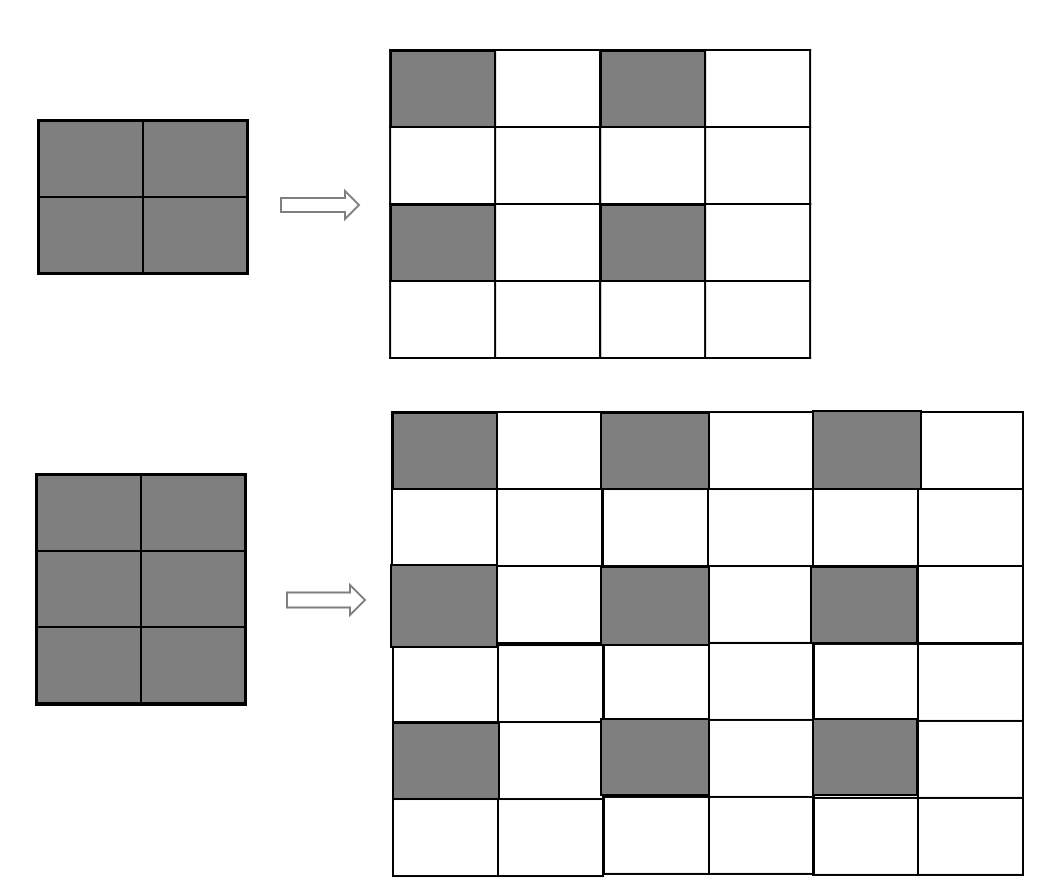
\includegraphics[scale=0.5]{figures/gan-unpooling.png}
\caption{小数跨步卷积}
\label{fig:gan-unpooling}
\end{figure}

2. 批量归一化

批量归一化是对每次训练的小批样本进行归一化处理,其优势为:可以让训练更简单高效、可以使用更大的学习率做为初始值、使模型对初始值更鲁棒、可以作为规范化操作、在一定程度上可以避免使用dropout操作、收敛速度加快。具体的,对于每个小批量输入,先通过\ref{equ:gan-batchnorm-mean}等式计算样本均值,通过\ref{equ:gan-batchnorm-std}等式计算样本标准差;然后通过等式\ref{equ:gan-batchnorm-x}对输入进行规范化;最后通过等式\ref{equ:gan-batchnorm-out}计算返回值。
\begin{subequations}
\begin{align}
\mu_{B} &= \frac{1}{m}\sum_{i=1}^{m}x^{(i)}\label{equ:gan-batchnorm-mean}\\
\sigma_{B}^{2} &= \frac{1}{m}\sum_{i=1}^{m}(x^{(i)}-\mu_{B})^{2} \label{equ:gan-batchnorm-std}\\
\hat{x}^{(i)} &= \frac{x^{(i)}-\mu_{B}}{\sqrt{\sigma_{B}^{2}+\epsilon }} \label{equ:gan-batchnorm-x}\\
z^{(i)} &= \gamma \hat{x}^{(i)} + \beta \label{equ:gan-batchnorm-out}
\end{align}
\end{subequations}

 (2)TSGAN的生成器

图\ref{fig:gan-ts-generator}是TSGAN的生成器。输入为随机产生的一维噪音向量$z$,其长度为$0.7*n$,其中$n$表示真实数据集中时间序列的长度(采样点个数)。首先通过变形或映射操作将输入转成3维矩阵,然后经过4层小数跨步卷积运算得到最后的输出,输出是长度为$n$的生成样本。其中每一次小数跨步卷积运算后会进行批量归一化,隐藏层的激活函数为ReLU,输出层为线性单元。卷积核统一为1*5规模。步长统一为2,即每一次小数跨步卷积运算实现2倍的升维。
% 最后输出层必须是线性单元!很关键!

\begin{figure}[H]
\centering
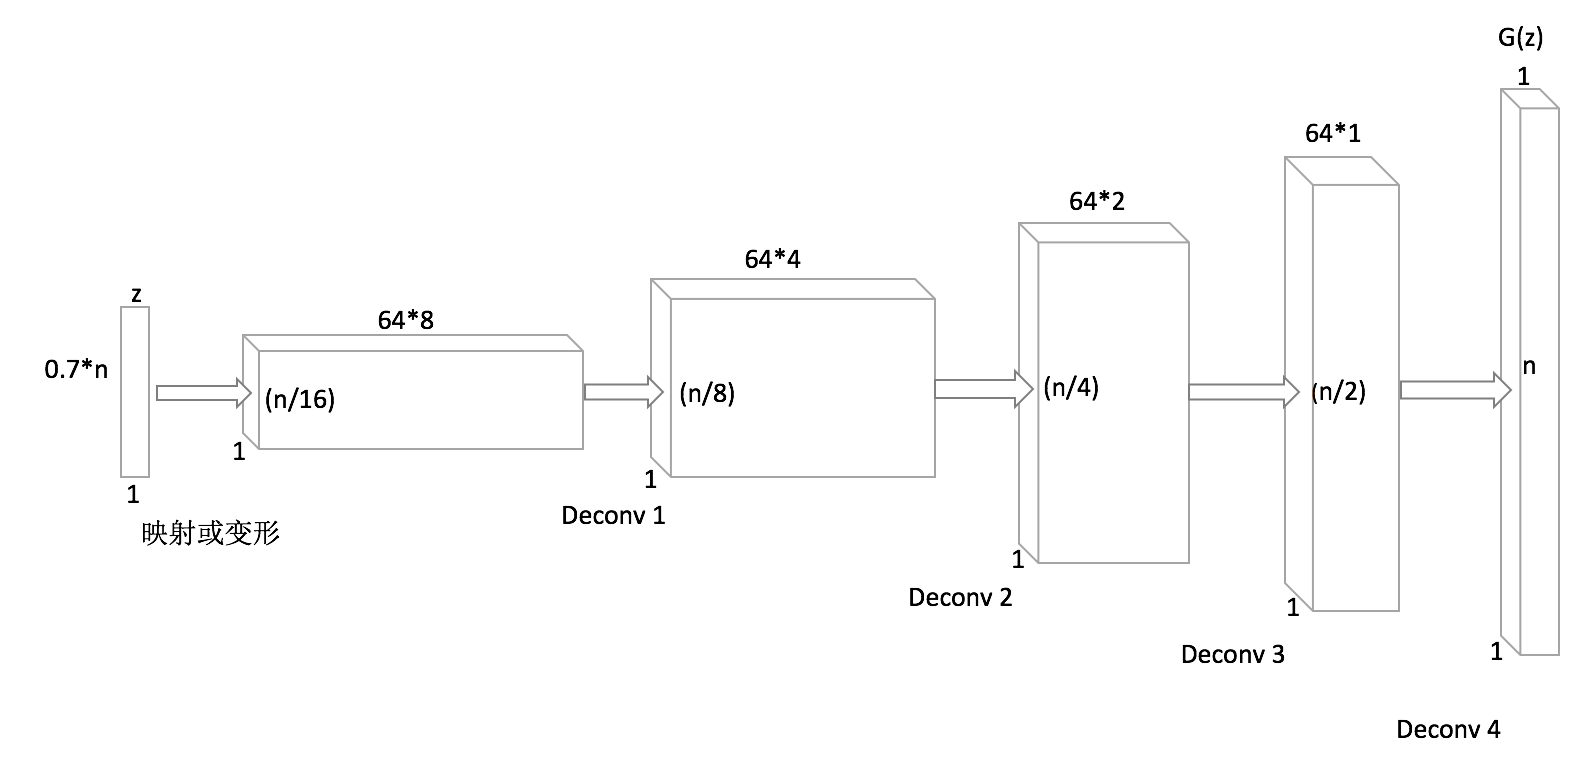
\includegraphics[scale=0.5]{figures/gan-ts-generator.png}
\caption{TSGAN 的生成器}
\label{fig:gan-ts-generator}
\end{figure}

(3)TSGAN的判别器

图\ref{fig:gan-ts-discriminator}是TSGAN的判别器。对输入长度为$n$的样本,通过4层卷积层,最后通过压平(flatten)操作得到一维特征向量,最后使用Sigmoid作为输出层实现二分类,输出是样本为真的概率。网络中不使用任何池化操作,降维通过无填补操作的卷积运算实现。其中卷积运算后进行批量归一化。所有隐藏层使用LeakyReLU作为激活函数。卷积核统一为1*5规模。步长统一为2,即每一次卷积运算实现2倍的降维。

\begin{figure}[H]
\centering
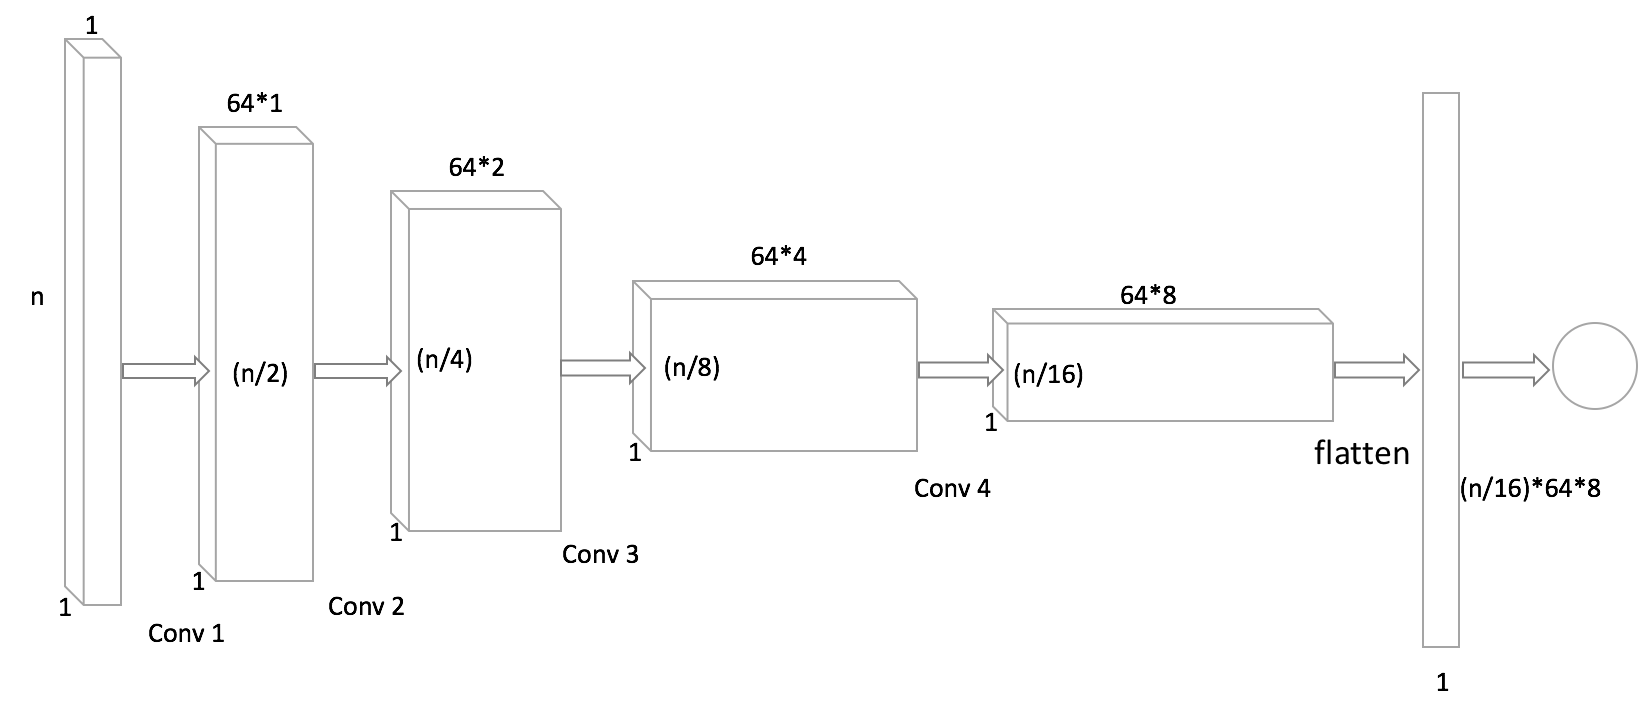
\includegraphics[scale=0.5]{figures/gan-ts-discriminator.png}
\caption{TSGAN 的判别器}
\label{fig:gan-ts-discriminator}
\end{figure}


(4)TSGAN的训练

\begin{algorithm}[H]
 \caption{基于随机梯度下降算法训练TSGAN}
 \KwData{判别器的更新次数dk,生成器的更新次数gk,训练迭代次数 epoch}
 \For{i=0; i<epoch; i++}{
  \For{j=0; j<dk; j++}{
    \ 从$p_{g}(z)$先验分布采样 ,$\{z^{(1)}, ...., z^{(m)}\}$\;
    \ 从真实样本$p_{data}(x)$中采样,$\{x^{(1)}, ..., x^{(m)}\}$\; 
    \ 基于梯度下降算法更新判别器:$\bigtriangledown _{\theta_{d}} -\frac{1}{m}\sum_{i=1}^{m}[log(D(x^{(i)})) + log(1-D(G(z^{(i)})))]$
  }
  \For{j=0; j<gk; j++}{
    \ 从$p_{g}(z)$先验分布采样 ,$\{z^{1}, ...., z^{m}\}$\;
    \ 基于梯度下降算法更新生成器:$\bigtriangledown _{\theta_{g}} -\frac{1}{m}\sum_{i=1}^{m}log(D(G(z^{i})))$ \;
  }
 }
 \renewcommand{\algorithmcfname}{算法}
 \label{gan-tsgan-algorithm}
\end{algorithm}

(5)TSGAN的评估

令真实数据集为$Y = \{y^{(1)}, ..., y^{(m)}\}$, 生成数据集为$X=\{x^{(1)}, ...., x^{(n)}\}$。本文采用最近邻距离(Nearest Neighbour Distance, NND)和最大平均差异(Maximum Mean Discrepancy, MMD)度量生成数据集和真实数据集的距离\cite{esteban2017real}。距离越小说明生成数据和真实数据越相似,进而说明生成器的性能越好。

1. 最近邻距离(NND)

最近邻距离(NND)的定义如等式\ref{equ:gan-metrics-nnd},先计算每个生成样本到真实数据集的距离,然后求和,最后取平均。

\begin{equation}
\label{equ:gan-metrics-nnd} 
NND = \frac{1}{n}\sum_{i=1}^{n}min_{j=1,...,m}\left \| x^{(i)} - y^{(j)} \right \|^{2}
\end{equation}

2. 最大平均差异(MMD)

生成式对抗网络的本质是学习数据的分布,因此通过度量生成数据集和真实数据集分布的相似性可以反映生成器生成数据的质量。MMD 通过度量两个数据集统计信息的差异的平方(表示为$MMD^{2}$)来衡量两个数据集的距离,并且将两个样本之间的点积替换成核函数$K: X \times Y \rightarrow \mathbb{R}$。$MMD^{2}$的无偏估定义如等式\ref{equ:gan-metrics-mmd},其中核函数使用基于L2距离的径向积函数(Radial Basis Function, RBF),即$K(x, y) = exp(-\left \| x-y \right \|^{2} / (2\sigma ^{2}))$。
\begin{equation}
\label{equ:gan-metrics-mmd} 
\hat{MMD}^{2} = \frac{1}{n(n-1)}\sum_{i=1}^{n}\sum_{j\neq i}^{n}K(x^{(i)}, x^{(j)})  - \frac{2}{nm}\sum_{i=1}^{n}\sum_{j=1}^{m}K(x^{(i)}, y^{(j)})+ \frac{1}{m(m-1)}\sum_{i=1}^{m}\sum_{j\neq i}^{m}K(y^{(i)}, y^{(j)}) 
\end{equation}

\section{无监督式时间序列特征应用}

TSGAN 通过无监督的方式进行训练后,一方面生成器学习了真实数据集的分布,可作为模拟器用于数据生成;另一方面判别器可作为特征转换器(类似于自编码机的编码器)与监督式学习任务融合形成半监督式学习框架,支持分类,预测、聚类、切割、索引、异常检测和主题发现等机器学习任务。本文选取时间序列分类任务,因为分类优劣直接依赖于特征的质量,可作为无监督式特征学习方法的有效检验手段。

图\ref{fig:gan-semi-supervised-learning}是基于TSGAN判别器的半监督式学习框架,输入的原生时间序列通过逐层运算后映射为一维特征向量以支持具体的机器学习任务。TSGAN的判别器总共有4次卷积运算,每次卷积运算都产生了一个特征矩阵,本文对后3个特征矩阵进行应用,丢弃第1个低维特征。直接拼接以上特征矩阵维度过高,因此本文将每一个特征矩阵接入池化层并通过最大池化操作对特征进行规约。

首先,基于层次越深,特征抽象层次越高,特征越有价值的启发式认识,假设每一层输入的特征矩阵高度为$h$,对于由浅到深的三个特征矩阵,本文依次使用规模为 $h/2$, $h/3$, $h/4$ 的滑窗进行最大池化规约运算。然后通过压平操作将特征矩阵转换成一维特征向量。最后将三个特征向量进行拼接形成对原生时间序列的新表示。

本文将通过以上操作获取的特征向量输入到基于欧式距离的1近邻(ED-1NN)、基于线性核函数的支持向量机(LinearSVM)和逻辑斯蒂回归(LR)简单分类器中实现时间序列分类任务。值得一提的是,本文采用简单分类器是为了体现TSGAN所学特征的有效性,ED-1NN是时间序列分类任务的基线、LinearSVM和LR通常是验证无监督式特征学习效果的通用基线。

\begin{figure}[H]
\centering
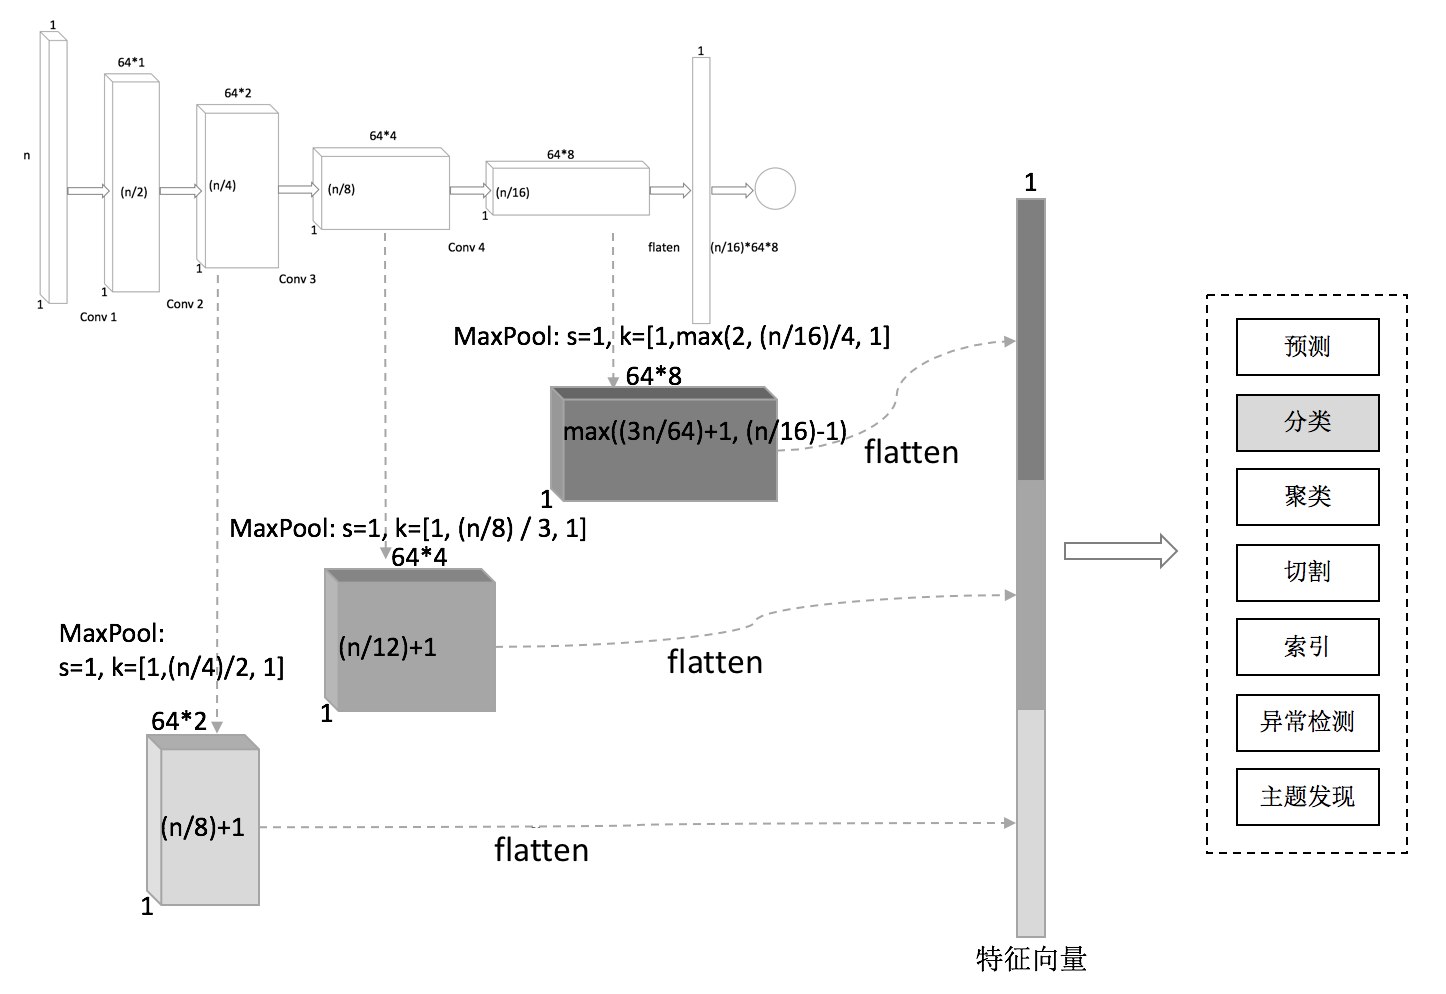
\includegraphics[scale=0.6]{figures/gan-semi-supervised-learning.png}
\caption{TSGAN的判别器作为特征转换器形成的半监督式学习框架}
\label{fig:gan-semi-supervised-learning}
\end{figure}

假设有训练集$Train = \{(x^{(1)}, y^{(1)}), (x^{(2)}, y^{(2)}), ..., (x^{(m)}, y^{(m)})\}$和测试集$Test = \{(x^{(1)}, y^{(1)}), (x^{(2)}, y^{(2)}), ..., (x^{(n)}, y^{(n)})\}$

(1)基于欧式距离的1近邻(ED-1NN) 

ED-1NN 分类算法没有训练过程,对于每个测试样本$(x,y)$的预测可分为两步:(a)计算$x$到训练集中每个样本的距离,即$d^{(i)} = \left \| x-x^{(i)} \right \|^{2},i=1,2,...,m$;(b)计算$x$的预测值$\hat{y}$,$\hat{y}$是距离最近的训练样本对应的类标,即$\hat{y}=y^{(i)}=argmin_{i \in \{1,2,...,m\}}d^{(i)}$。

重复以上两个步骤$n$次即可获得所有测试样本的估计值。

(2)基于线性核函数的支持向量机(LinearSVM)

标准的LinearSVM是一个二分类器,其损失函数为$J(\theta) = \lambda\sum_{1}^{m}max(0, 1-y^{(i)}(w^{T}x^{(i)}+b)) +  \frac{1}{2}\left \| w \right \|^{2}$,其中$\lambda$为惩罚因子。

对于多分类问题,假设有$C$个类,对每个类$c \in \{1,2,...,C\}$训练一个标准LinearSVM二分类器,由此得到$C$个二分类器分别对应的$C$组参数,即$\{(w^{(1)}, b^{(1)}), (w^{(2)}, b^{(2)}), ...., (w^{(C)}, b^{(C)})\}$。那么预测的估计值为$\hat{y} = argmax_{c}((w^{(c)})^{T}x+b^{(c)})$

(3)逻辑斯蒂回归(LR)

标准的LR是二分类器,对于任意样本$(x,y)$,其中$y \in {0,1}$,0表示负例,1表示正例,LR的训练过程如下:(a) LR根据等式$h_{\theta}(x) = \frac{1}{1+e^{-\theta^{T}x}}, h_{\theta}(x) = [0,1]$计算每个样本$x$为正例的概率;(b) LR根据损失函数$J(\theta) = -\frac{1}{m}[\sum_{1}^{m}y^{(i)}log(h_{\theta}(x^{(i)}))+(1-y^{(i)})log(1-h_{\theta}(x^{(i)}))] + \frac{1}{2}\left \| \theta \right \|^{2}$ 训练模型。(c)在预测阶段,对每个样本x计算其属于正样本的概率$h_{\theta}(x^{(i)}), i=1,...n$,如果概率大于等于0.5,则预测类标为1,否则为0。

对于多分类问题,假设有$C$个类。对每个类$c \in \{1,2,...,C\}$训练一个二分类器$ h_{\theta}^{c}(x)$,此时所有$y=c$的样本都为正例,其他样本都被看作是负例。预测时,$ \hat{y} = argmax_{c} h_{\theta}^{c}(x)$,即$C$个分类器中输出概率最大的那个分类器的类标将作为当前样本的预测值。

(4)分类效果评估

通过分类准确率来衡量分类的效果,具体定义为$acc = \frac{1}{m}\sum_{i=1}^{m}\mathbb{I}(h(x^{(i)}) = y^{(i)})$,其中$\mathbb{I}$为指示函数,当传入的表达式为真时取值为1,否则取值为0。


\section{实验结果与分析}

本文使用最大的时间序列分类公开数据集UCR\cite{bagnall16bakeoff}进行实验。UCR总共包含85个时间序列数据集,每个数据集都由若干类别的单元时间序列构成。本文根据数据特性,将UCR数据集划分为以下几类:采集自工业系统的时间序列数据集、基于加速计采集的运动时间序列数据集、基于形状的时间序列数据集、基于传感器采集的频谱时间序列数据集和医疗时间序列数据集。

实验硬件的主要参数:CPU,Intel(R) Xeon(R) CPU E5-2682,16 核,2.50GHz;内存,235GB;GPU,Tesla P100 PCIe,16GB。所有算法均使用 Python 3.6.0 实现,主要依赖库有,TSGAN模型实现依赖 TensorFlow 1.4.0,简单分类器模型实现依赖 scikit-learn 0.19.1。针对所有数据集的训练,除输入层和输出层外均采用统一配置,其中模型结构及相应参数参见本章\ref{tsgan-model};训练参数,采用Adam梯度下降算法,生成器和判别器的初始学习率都是0.0002,训练迭代次数为200,判别器和生成器的更新频率是1:1。训练集和测试集的划分和公开数据集的划分一致。

通过算法\ref{gan-tsgan-algorithm}对TSGAN进行无监督式训练后,一方面TSGAN的生成器已拟合真实数据分布,可作为模拟器使用;另一方面,TSGAN的判别器已学习真实数据的有效映射,可作为特征转换器与简单分类器结合完成时间序列分类任务。

(1)TSGAN生成器生成时间序列数据的效果展示

除了可视化展示生成数据外,本文还采用NND和MMD指标评估生成样本的质量,即对于每个数据集,首先通过TSGAN生成器产生 100000 条时间序列样本构成生成数据集,然后计算生成数据集和真实测试集之间的NND和MMD距离。由于数据集较多,本文每一类数据集展示一组示例。

1. 采集自工业系统的时间序列数据集。如图\ref{fig:gan-show-FordA}为数据集FordA的生成结果。FordA是汽车子系统运行状态下的引擎噪音信号,是2008年电气和电子工程师协会(Institute of Electrical and Electronics Engineers, IEEE)计算智能世界大会的时间序列分类竞赛数据集。竞赛任务为识别某种特定症状是否存在于汽车子系统中,因此FordA包含两类时间序列(正常数据和故障数据),是典型的故障分类问题。\ref{fig:gan-show-FordA}a是输入生成器的随机噪音;\ref{fig:gan-show-FordA}b是从生成数据集中随机抽取的6个样本,\ref{fig:gan-show-FordA}c是从真实数据集中随机抽取的6个样本,可以看到生成时间序列和真实时间序列非常相似,难以分辨真假;\ref{fig:gan-show-FordA}d是判别器和生成器的损失函数,保持平稳;\ref{fig:gan-show-FordA}e是NND距离,\ref{fig:gan-show-FordA}f是MMD距离,可以看到随着训练次数的叠加,距离指标不断减小,说明生成数据集和真实数据集越来越相似,最后趋于平稳。 
%This data was originally used in a competition in the IEEE World Congress on Computational Intelligence, 2008. The classification problem is to diagnose whether a certain symptom exists or does not exist in an automotive subsystem. Each case consists of 500 measurements of engine noise and a classification. There are two separate problems: For FordA the Train and test data set were collected in typical operating conditions, with minimal noise contamination.

2. 基于传感器采集的频谱时间序列数据集。如图\ref{fig:gan-show-InsectWingbeatSound}为数据集InsectWingbeatSound的生成结果。InsectWingbeatSound是通过传感器采集的昆虫振翅声的功率频谱,是11类雄性和雌性蚊子的采样结果。

3. 基于形状的时间序列数据集。如图\ref{fig:gan-show-ArrowHead}为数据集ArrowHead的生成结果,ArrowHead是通过极坐标将三类箭头图片映射而成的时间序列。
%基于形状的时间序列是一种典型的数据类型,通过某种映射方式将图片、文字等物体影射为一维时间序列。

4. 基于加速计采集的运动时间序列数据集。如图\ref{fig:gan-show-uWaveGestureLibrary_Z}为数据集uWaveGestureLibrary\_Z的生成结果。uWaveGestureLibrary\_Z是通过加速计采集的8类手势运动数据。

5. 医疗时间序列数据集。如图\ref{fig:gan-show-ECGFiveDays}为数据集ECGFiveDays的生成结果,是2类心电图信号。

实验结果证明TSGAN的生成器学习了真实时间序列数据集的分布,并生成逼真的多样化的时间序列。

% Device
\begin{figure}[H]
\centering
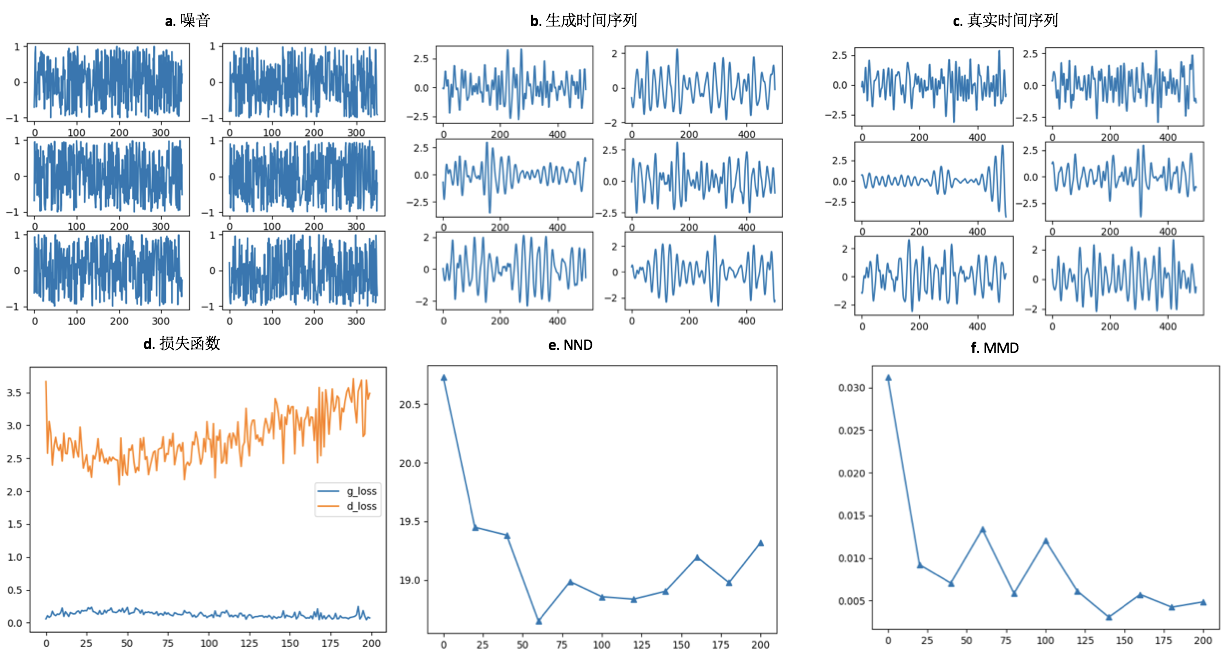
\includegraphics[scale=0.5]{figures/gan/FordA.png}
\caption{FordA 数据集的生成结果}
\label{fig:gan-show-FordA}
\end{figure}
% spectrograms
\begin{figure}[H]
\centering
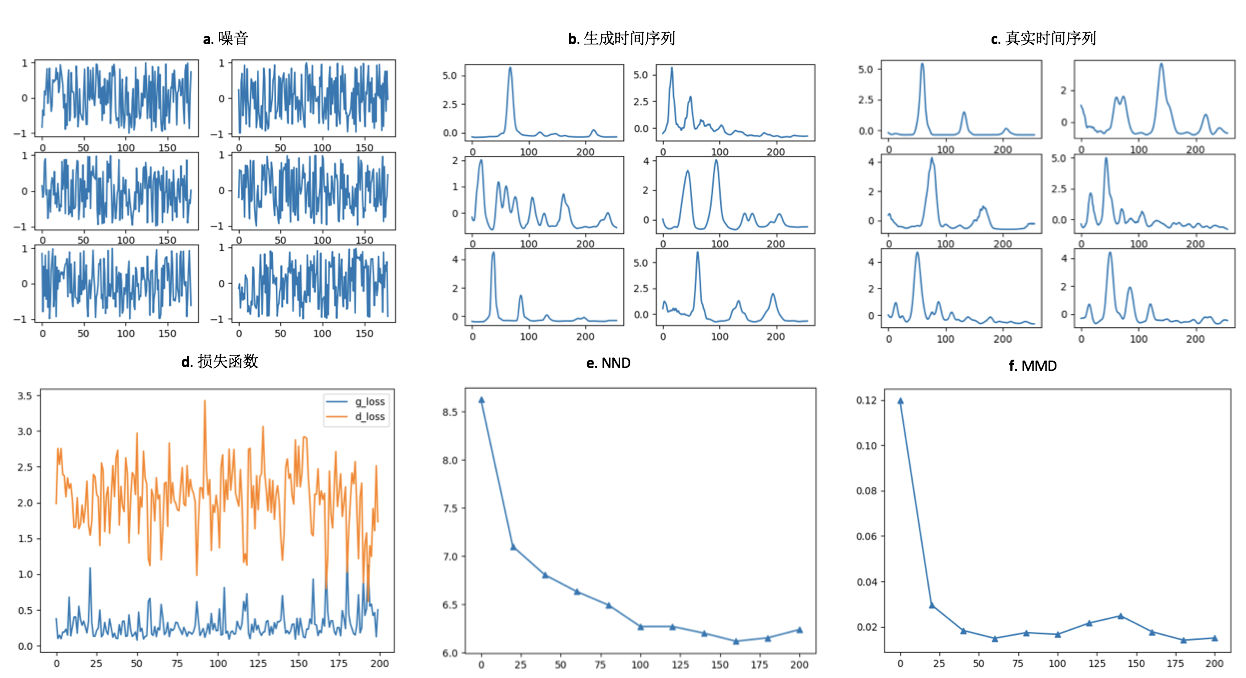
\includegraphics[scale=0.5]{figures/gan/InsectWingbeatSound.png}
\caption{InsectWingbeatSound 数据集的生成结果}
\label{fig:gan-show-InsectWingbeatSound}
\end{figure}
% Shape
\begin{figure}[H]
\centering
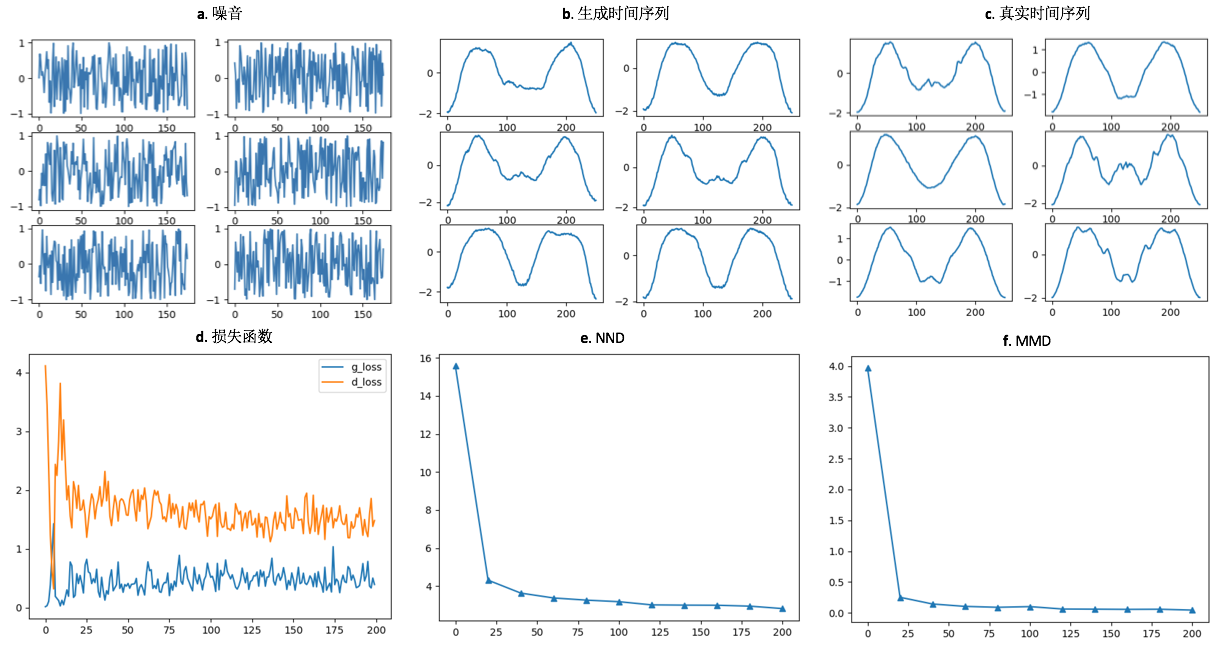
\includegraphics[scale=0.5]{figures/gan/ArrowHead.png}
\caption{ArrowHead 数据集的生成结果}
\label{fig:gan-show-ArrowHead}
\end{figure}
% accelerometers ---- motion
\begin{figure}[H]
\centering
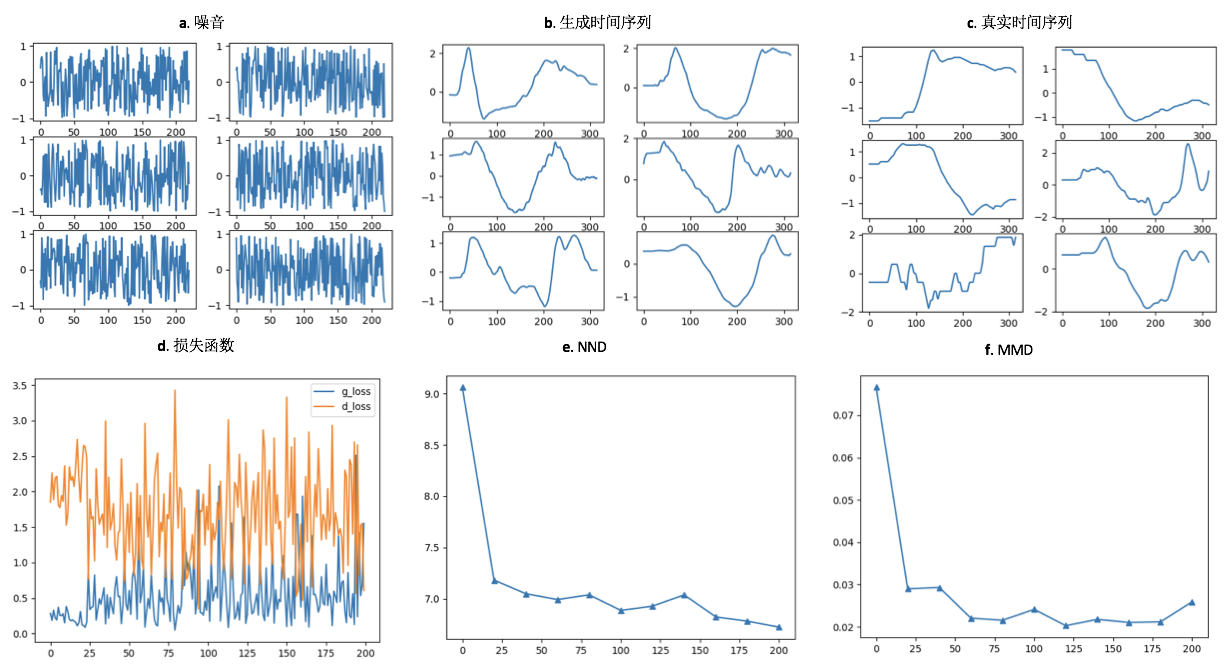
\includegraphics[scale=0.5]{figures/gan/uWaveGestureLibrary_Z.png}
\caption{uWaveGestureLibrary\_Z 数据集的生成结果}
\label{fig:gan-show-uWaveGestureLibrary_Z}
\end{figure}
% ECG
\begin{figure}[H]
\centering
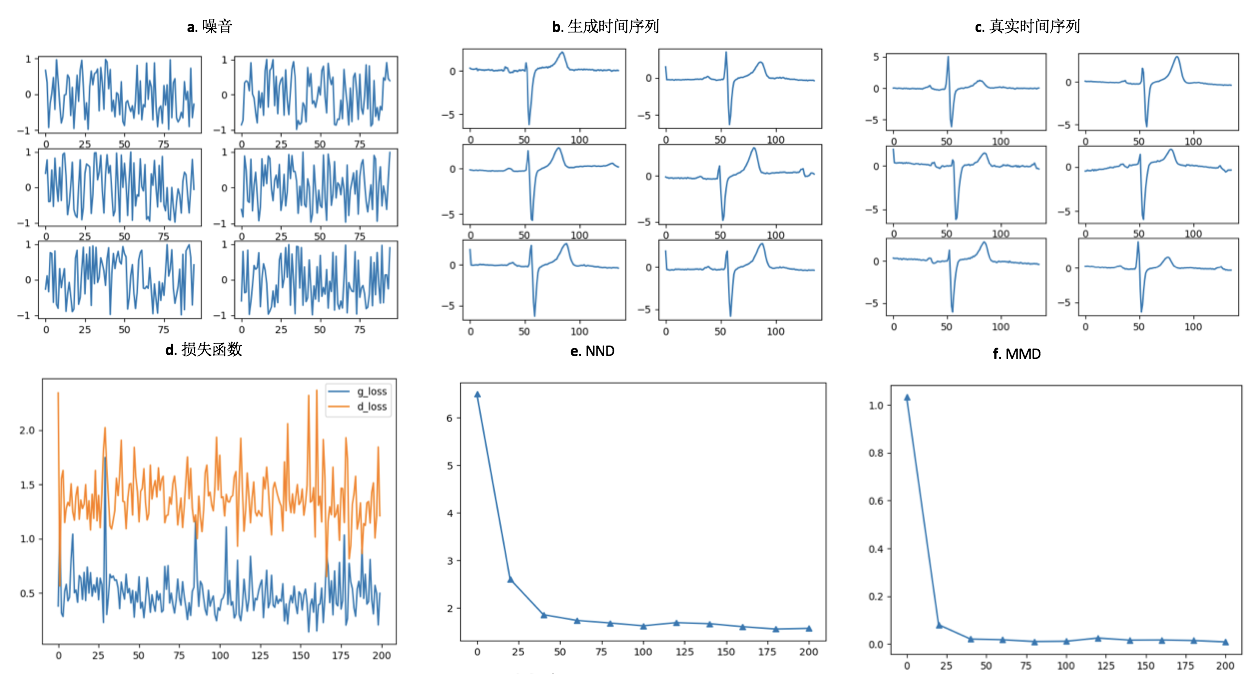
\includegraphics[scale=0.5]{figures/gan/ECGFiveDays.png}
\caption{ECGFiveDays 数据集的生成结果}
\label{fig:gan-show-ECGFiveDays}
\end{figure}


(2)基于TSGAN判别器的半监督式时间序列分类结果

经过无监督式训练后的TSGAN,其判别器已通过博弈的方式学习了真实数据集的有效特征映射,可以将输入的原生时间序列映射到有利于后续任务的特征向量。如图\ref{fig:gan-semi-supervised-learning},本文将TSGAN的判别器作为特征转换器分别与ED-1NN、LinearSVM和LR简单分类器结合,构建半监督式学习框架。表\ref{tab:gan-classify}对比是否有TSGAN特征转换器的分类效果,可以看到有TSGAN特征转换器的情况下分类准确率更高。图\ref{fig:gan-acc-knn},从左至右依次对应ED-1NN,LinearSVM和LR的分类对比结果,横坐标为基于原生时间序列的分类准确率,纵坐标为基于TSGAN特征转换器获取的特征向量的分类准确率,可以看到绝大部分的数据集都位于对角线上方,说明基于TSGAN特征转换器获取的特征向量的分类效果更好。以上结果充分说明TSGAN基于无标记数据可以学习数据的有效特征映射,并可基于此实现精确的分类。

值得一提的是,可以通过微调半监督式分类框架中TSGAN判别器模块实现进一步优化。
%Further improvements could be made by finetuning the discriminator’s representations, but we leave this for future work.

\begin{longtable}[c]{p{5cm}<{\centering}*{6}{c}}
\caption{分类结果}\label{tab:gan-classify}\\
\toprule[1.5pt]
数据集 & \multicolumn{2}{c}{1NN} & \multicolumn{2}{c}{LSVC} & \multicolumn{2}{c}{LR} \\
    & \multicolumn{1}{c}{原数据} & \multicolumn{1}{c}{GAN特征}& \multicolumn{1}{c}{原数据}& \multicolumn{1}{c}{GAN特征}& \multicolumn{1}{c}{原数据}&  \multicolumn{1}{c}{GAN特征} \\\midrule[1pt]
\endfirsthead
\multicolumn{7}{c}{续表~\thetable\hskip1em 分类结果}\\
\toprule[1.5pt]
数据集 & \multicolumn{2}{c}{1NN} & \multicolumn{2}{c}{LSVC} & \multicolumn{2}{c}{LR} \\
  & \multicolumn{1}{c}{原数据} & \multicolumn{1}{c}{GAN特征}& \multicolumn{1}{c}{原数据}& \multicolumn{1}{c}{GAN特征}& \multicolumn{1}{c}{原数据}&  \multicolumn{1}{c}{GAN特征} \\\midrule[1pt]
\endhead
\hline
\multicolumn{7}{r}{续下页}
\endfoot
\endlastfoot
50words &0.6308 &0.7297 &0.5011 &0.7758 &0.5341 &0.7758 \\
Adiac &0.6113 &0.7289 &0.6189 &0.7545 &0.6752 &0.79780 \\
ArrowHead &0.8000 &0.8286 &0.6743 &0.8 &0.765 &0.8171 \\
Beef &0.6667 &0.6000 &0.8667 &0.8333 &0.8667 &0.8333 \\
BeetleFly &0.7500 &0.6500 &0.8000 &0.8000 &0.8500 &0.8000 \\
BirdChicken &0.5500 &0.7000 &0.7500 &0.8000 &0.7500 &0.9000 \\
CBF &0.8522 &1.0000 &0.7122 &0.9944 &0.8344 &0.9944 \\
Car &0.7333 &0.7167 &0.8167 &0.8333 &0.8667 &0.8333 \\
ChlorineConcentration &0.6500 &0.8456 &0.7221 &0.9070 &0.8240 &0.9010 \\
CinC\_ECG\_torso &0.8971 &0.8913 &0.4551 &0.9072 &0.4964 &0.9275 \\
Coffee &1.0000 &1.0000 &1.0000 &1.0000 &1.0000 &1.0000 \\
Computers &0.5760 &0.5320 &0.5120 &0.6360 &0.5080 &0.6560 \\
Cricket\_X &0.5769 &0.6487 &0.2333 &0.7077 &0.2974 &0.7205 \\
Cricket\_Y &0.5667 &0.6513 &0.2333 &0.7410 &0.3692 &0.7462 \\
Cricket\_Z &0.5872 &0.6410 &0.2231 &0.7103 &0.2949 &0.7205 \\
DiatomSizeReduction &0.9346 &0.9542 &0.9706 &0.9706 &0.9608 &0.9608 \\
DistalPhalanxOutlineAgeGroup &0.7825 &0.7550 &0.7825 &0.7450 &0.8000 &0.8250 \\
DistalPhalanxOutlineCorrect &0.7517 &0.7750 &0.6967 &0.7983 &0.7000 &0.8300 \\
DistalPhalanxTW &0.7275 &0.7125 &0.7500 &0.7475 &0.7650 &0.7875 \\
ECG200 &0.8800 &0.9200 &0.8500 &0.8900 &0.8500 &0.8900 \\
ECG5000 &0.9249 &0.9251 &0.9340 &0.9427 &0.9418 &0.9464 \\
ECGFiveDays &0.7967 &0.7758 &0.9431 &0.8177 &0.9547 &0.8177 \\
Earthquakes &0.6739 &0.6894 &0.5963 &0.7733 &0.6087 &0.7888 \\
ElectricDevices &0.5487 &0.6159 &0.4526 &0.6571 &0.4643 &0.6866 \\
FISH &0.7829 &0.8343 &0.8686 &0.9314 &0.8571 &0.9257 \\
FaceAll &0.7136 &0.7385 &0.7787 &0.8089 &0.8118 &0.8041 \\
FaceFour &0.7841 &0.8409 &0.8750 &0.8750 &0.8636 &0.8864 \\
FacesUCR &0.7693 &0.8951 &0.7307 &0.9283 &0.7512 &0.9259 \\
FordA &0.6590 &0.8259 &0.4957 &0.9145 &0.5062 &0.9234 \\
FordB &0.5578 &0.8045 &0.4978 &0.8914 &0.5072 &0.9109 \\
Gun\_Point &0.9133 &0.9600 &0.8467 &0.9667 &0.8467 &0.9867 \\
Ham &0.6000 &0.5619 &0.6095 &0.6952 &0.7429 &0.7238 \\
HandOutlines &0.8010 &0.8280 &0.8430 &0.8680 &0.8590 &0.8790 \\
Haptics &0.3701 &0.3734 &0.3929 &0.4968 &0.4643 &0.5260 \\
Herring &0.5156 &0.5156 &0.6250 &0.6250 &0.6875 &0.6406 \\
InlineSkate &0.3418 &0.3327 &0.2291 &0.3618 &0.2782 &0.3655 \\
InsectWingbeatSound &0.5616 &0.4424 &0.5263 &0.6121 &0.6409 &0.6268 \\
ItalyPowerDemand &0.9553 &0.9514 &0.9708 &0.9417 &0.9689 &0.9582 \\
LargeKitchenAppliances &0.4933 &0.5813 &0.3413 &0.7013 &0.3867 &0.7040 \\
Lighting2 &0.7541 &0.7213 &0.6393 &0.6885 &0.6721 &0.6885 \\
Lighting7 &0.5753 &0.6849 &0.5068 &0.6712 &0.6164 &0.7260 \\
MALLAT &0.9143 &0.8938 &0.8874 &0.9156 &0.8823 &0.9326 \\
Meat &0.9333 &0.9333 &0.9667 &0.9667 &0.9833 &0.96667 \\
MedicalImages &0.6842 &0.6500 &0.6092 &0.6513 &0.6184 &0.7342 \\
MiddlePhalanxOutlineAgeGroup &0.7400 &0.7325 &0.7650 &0.7725 &0.8050 &0.7975 \\
MiddlePhalanxOutlineCorrect &0.7533 &0.7700 &0.5333 &0.7933 &0.5400 &0.8067 \\
MiddlePhalanxTW &0.5614 &0.5664 &0.6216 &0.6040 &0.6441 &0.6391 \\
MoteStrain &0.8786 &0.8299 &0.8634 &0.8610 &0.8658 &0.8674 \\
NonInvasiveFatalECG\_Thorax1 &0.8290 &0.8753 &0.9094 &0.94402 &0.9160 &0.9466 \\
NonInvasiveFatalECG\_Thorax2 &0.8799 &0.8794 &0.9328 &0.93893 &0.9399 &0.9425 \\
OSULeaf &0.5207 &0.7355 &0.4463 &0.8636 &0.4669 &0.8636 \\
OliveOil &0.8667 &0.8667 &0.5667 &0.1667 &0.8667 &0.8667 \\
PhalangesOutlinesCorrect &0.7611 &0.7984 &0.6702 &0.8030 &0.6702 &0.8333 \\
Phoneme &0.1092 &0.2964 &0.0854 &0.3412 &0.09388 &0.3518 \\
Plane &0.9619 &0.9714 &0.9905 &0.9810 &0.9905 &0.9905 \\
ProximalPhalanxOutlineAgeGroup &0.7854 &0.8244 &0.8439 &0.8244 &0.8634 &0.8585 \\
ProximalPhalanxOutlineCorrect &0.8076 &0.8316 &0.8247 &0.4742 &0.8454 &0.9003 \\
ProximalPhalanxTW &0.7075 &0.7300 &0.7900 &0.7600 &0.8050 &0.8075 \\
RefrigerationDevices &0.3947 &0.5227 &0.3520 &0.5307 &0.3680 &0.5440 \\
ScreenType &0.3600 &0.3573 &0.3733 &0.3920 &0.3947 &0.4160 \\
ShapeletSim &0.5389 &0.6722 &0.4944 &0.6444 &0.4944 &0.6444 \\
ShapesAll &0.7517 &0.8417 &0.5900 &0.8750 &0.6168 &0.8750 \\
SmallKitchenAppliances &0.3440 &0.5920 &0.3413 &0.7173 &0.4027 &0.7280 \\
SonyAIBORobotSurface &0.6955 &0.6439 &0.7304 &0.7937 &0.7338 &0.7887 \\
SonyAIBORobotSurfaceII &0.8594 &0.87408 &0.8416 &0.9297 &0.8332 &0.9297 \\
StarLightCurves &0.8488 &0.9261 &0.8623 &0.9681 &0.9042 &0.9757 \\
Strawberry &0.9380 &0.9478 &0.9527 &0.9364 &0.9641 &0.9788 \\
SwedishLeaf &0.7888 &0.8864 &0.768 &0.9552 &0.7696 &0.9600 \\
Symbols &0.8995 &0.9618 &0.7568 &0.9668 &0.7889 &0.9658 \\
ToeSegmentation1 &0.6798&0.7544 &0.5482 &0.9079 &0.5877 &0.9211 \\
ToeSegmentation2 &0.8077 &0.8385 &0.5462 &0.9231 &0.5462 &0.9231 \\
Trace &0.7600 &0.9900 &0.7300 &1.0000 &0.7300 &1.0000 \\
TwoLeadECG &0.7471 &0.9631 &0.9263 &0.9570 &0.9263 &0.9579 \\
Two\_Patterns &0.9068 &0.8815 &0.8020 &0.9938 &0.8083 &0.9918 \\
UWaveGestureLibraryAll &0.9481 &0.8752 &0.7552 &0.9548 &0.8453 &0.9537 \\
Wine &0.6111 &0.7037 &0.5926 &0.5000 &0.8519 &0.8704 \\
WordsSynonyms &0.6176 &0.6897 &0.4154 &0.6912 &0.4561 &0.6991 \\
Worms &0.3646 &0.4862 &0.2873 &0.5304 &0.3039 &0.5414 \\
WormsTwoClass &0.5856 &0.6906 &0.4972 &0.7182 &0.5193 &0.7403 \\
synthetic\_control &0.8800 &1.0000 &0.7833 &0.9967 &0.8267 &0.9933 \\
uWaveGestureLibrary\_X &0.739 &0.8023 &0.6164 &0.8313 &0.6387 &0.8467 \\
uWaveGestureLibrary\_Y &0.6616 &0.7247 &0.5011 &0.7451 &0.5765 &0.7599 \\
uWaveGestureLibrary\_Z &0.6496 &0.7295 &0.5134 &0.7610 &0.5497 &0.7714 \\
wafer &0.9955 &0.9933 &0.9431 &0.9976 &0.9414 &0.9974 \\
yoga &0.8303 &0.8260 &0.6460 &0.8483 &0.6543 &0.8477 \\
\bottomrule[1.5pt]
\end{longtable}

% \begin{figure}[H]
% \centering
% 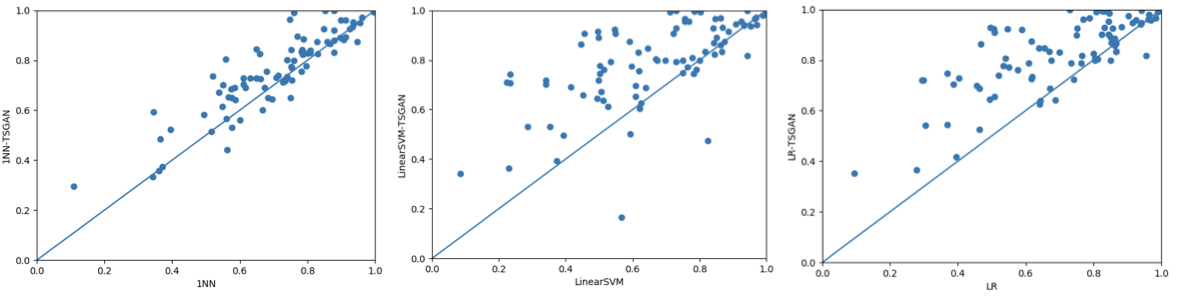
\includegraphics[scale=0.8]{figures/gan/acc.png}
% \caption{分类比较结果}
% \label{fig:gan-acc-knn}
% \end{figure}

% \begin{figure}[H]
% \centering
% 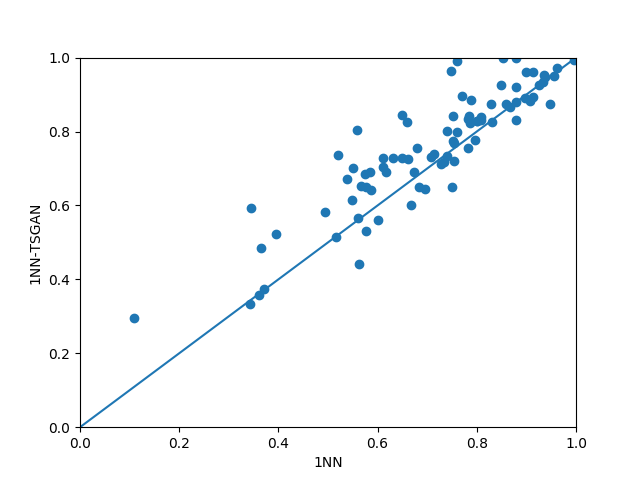
\includegraphics[scale=0.8]{figures/gan/0000_acc_knn.png}
% \caption{ED-1NN 分类比较结果}
% \label{fig:gan-acc-knn}
% \end{figure}

% \begin{figure}[H]
% \centering
% 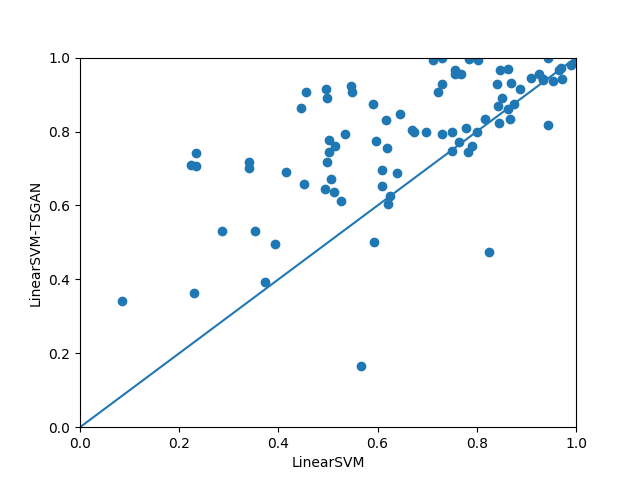
\includegraphics[scale=0.8]{figures/gan/0000_acc_lsvc.png}
% \caption{LinearSVM 分类比较结果}
% \label{fig:gan-acc-lsvc}
% \end{figure}

% \begin{figure}[H]
% \centering
% \includegraphics[scale=0.8]{figures/gan/0000_acc_lr.png}
% \caption{LR 分类比较结果}
% \label{fig:gan-acc-lr}
% \end{figure}

\section{小结}

本章针对高质量工业时间序列标记数据获取难的问题,基于生成式对抗网络提出了无监督式时间序列通用特征学习模型TSGAN,并通过最大的时间序列分类数据集(85个数据集)进行实验。一方面,TSGAN的生成器学习了真实数据集的分布,并生成逼真的多样化的时间序列,可作为模拟器使用;另一方面,将TSGAN的判别器作为特征转换器与简单分类器结合,构建了半监督式时间序列分类模型,并且取得了优秀的分类效果。

% # data parameter
% self.X = X
% self.img_h = img_h
% self.img_w = img_w
% self.c_dim = c_dim
% self.z_dim = int(X.shape[1] * 0.7)
% #self.z_dim = 100
% # model parameter
% self.gf_dim = 64  # dimension of G filters in first conv layer
% self.df_dim = 64  # dimension of D filters in first conv layer
% # training parameter
% self.nbatch = min(20, len(self.X))
% self.g_learning_rate = 0.0002
% self.d_learning_rate = 0.0002
% self.g_beta1 = 0.5
% self.d_beta2 = 0.5
% self.nepoch = 200
% self.k = 1
% # log parameter
% self.data_name = data_name
% self.file_name = out_fname
% self.model_name = "{}_{}".format(self.file_name, self.data_name)
% self.freq_print = 1
% self.freq_plot = 20
% self.freq_log = 20
% self.nsample = 10000
% self.dir_root = '/home/hfl/dataset/output/gan_timeseries_tf/{}'.format(self.file_name)
% self.dir_root_dataset = '{}/{}'.format(self.dir_root, self.data_name)
% self.dir_logs = os.path.join(self.dir_root_dataset, 'logs')
% self.dir_samples = os.path.join(self.dir_root_dataset, 'samples')
% self.dir_checkpoint = os.path.join(self.dir_root_dataset, 'checkpoint')

% # construct log file
% if state == 'train':
%     if os.path.exists(self.dir_root_dataset):
%         shutil.rmtree(self.dir_root_dataset)
%     os.makedirs(self.dir_root_dataset)
%     os.makedirs(self.dir_logs)
%     os.makedirs(self.dir_samples)
%     os.makedirs(self.dir_checkpoint)

% !TEX root = ../main.tex

\chapter{总结与展望}
\label{chap:conclusion}

本文针对“高维、高噪、时变”时间序列数据的特征学习以及其在工业装备运维中的作用进行了系统研究。主要研究工作如下:

1. 提出了基于符号回归的系统结构特征学习方法并展开应用。利用以轴温为代表的设备正常态运行数据展开研究;学习了系统结构特征,揭示了轴承的动态性和信号间的相互作用关系;将最优系统结构特征作为系统运行时的健康基线,设计了在线实时异常检测框架。

2. 提出了基于复杂系统临界相变理论的早期预警特征学习方法并展开应用。利用来自4个不同工业系统的系统全生命周期数据开展研究;学习了具有普适性的系统失效早期预警特征;针对早期特征,提出了关键跳变检测算法实现故障预测。

3. 提出了基于生成式对抗网络的无监督式时间序列特征学习模型——TSGAN,并展开应用。利用最大的时间序列分类数据集(85个数据集)开展研究;一方面,TSGAN 的生成器学习了真实数据集的分布,作为模拟器使用,生成了逼真的多样化的时间序列;另一方面,将TSGAN的判别器作为特征转换器与简单分类器结合构建了半监督式时间序列分类框架,并取得优秀效果。

未来工作展望:

1. 对基于符号回归的系统结构特征学习框架进一步优化。一方面,当前的方法存在产生冗余运算子的情况,仍有进一步优化的空间。另一方面,尝试融合更多的学习策略或模型进一步提高现有框架的数据和环境自适应能力。

2. 对复杂系统临界相变预测理论的更多探索。一方面,基于现有发现研究通用方法来预测和预防系统失效很有意义。另一方面,探索更多的方法,尤其是先进的机器学习方法,发现更多临界相变普适特征很有吸引力。

3. 对TSGAN的进一步改进和应用。一方面,通用配置的TSGAN对少量的极端验证集(比如高噪振动信号)仍不够鲁棒,因此可以尝试更多的神经网络结构或优化方法对TSGAN进行改进;另一方面,TSGAN作为特征转换器,不仅可以支持时间序列分类,还可以尝试与更多的任务结合,比如聚类、切割、索引、异常检测、主题发现等任务。

4. 临界相变理论和生成式模型的结合。一方面,临界相变理论揭示了系统底层失效机理,若看似不同的系统可以临界相变理论为媒介实现互联互通,将具有领域突破性意义;另一方面,生成式模型具有学习数据底层分布的能力,可对无标记数据进行利用,若能通过生成式模型揭示数据底层共享特征域并基于此实现不同数据间的转换,将有可能大幅度缓解标记数据缺乏问题。探索以上任一个方面或综两方面的研究都极具吸引力。

%5. 时间序列特征学习方法,尤其是无监督式时间序列特征学习方法的深入。特征学习是机器学习和数据挖掘的关键,本文的研究只涉及


%%% 其它部分
\backmatter

%% 本科生要这几个索引,研究生不要。选择性留下。
% 插图索引
%\listoffigures
% 表格索引
%\listoftables
% 公式索引
%\listofequations


%% 参考文献
% 注意:至少需要引用一篇参考文献,否则下面两行可能引起编译错误。
% 如果不需要参考文献,请将下面两行删除或注释掉。
% 数字式引用
\bibliographystyle{thuthesis-numeric}
% 作者-年份式引用
% \bibliographystyle{thuthesis-author-year}
\bibliography{ref/refs}


%% 致谢
% 如果使用声明扫描页,将可选参数指定为扫描后的 PDF 文件名,例如:
% \begin{acknowledgement}[scan-statement.pdf]
\begin{acknowledgement}
  首先由衷感谢我的导师邓仰东老师,感谢导师一直以来的悉心指导和栽培。全文工作均在导师指导下完成,论文工作开展过程中遇到过许多困难和瓶颈,得到了导师的诸多帮助、启发和鼓励。世界上最快乐的事之一可谓探索真知的过程,导师对探索真知的热情与严谨求证的态度深深感染和鼓舞着我,使我受用终生。

  感谢同一研究所的黄晋老师,黄晋老师对智慧交通有很深的见解,在具体工程实践环节给予了诸多启示。

  感谢学校和实验室给予的良好学习及科研氛围。

  感谢家人一直以来的鼓励和支持。

  % 衷心感谢导师 xxx 教授和物理系 xxx 副教授对本人的精心指导。他们的言传身教将使
  % 我终生受益。

  % 在美国麻省理工学院化学系进行九个月的合作研究期间,承蒙 xxx 教授热心指导与帮助,不
  % 胜感激。感谢 xx 实验室主任 xx 教授,以及实验室全体老师和同学们的热情帮助和支
  % 持!本课题承蒙国家自然科学基金资助,特此致谢。

  % 感谢 \LaTeX 和 \thuthesis\cite{thuthesis},帮我节省了不少时间。
\end{acknowledgement}


%% 附录
% \begin{appendix}
% % \chapter{外文资料原文}
% \label{cha:engorg}

% \title{The title of the English paper}

% \textbf{Abstract:} As one of the most widely used techniques in operations
% research, \emph{ mathematical programming} is defined as a means of maximizing a
% quantity known as \emph{bjective function}, subject to a set of constraints
% represented by equations and inequalities. Some known subtopics of mathematical
% programming are linear programming, nonlinear programming, multiobjective
% programming, goal programming, dynamic programming, and multilevel
% programming$^{[1]}$.

% It is impossible to cover in a single chapter every concept of mathematical
% programming. This chapter introduces only the basic concepts and techniques of
% mathematical programming such that readers gain an understanding of them
% throughout the book$^{[2,3]}$.


% \section{Single-Objective Programming}
% The general form of single-objective programming (SOP) is written
% as follows,
% \begin{equation}\tag*{(123)} % 如果附录中的公式不想让它出现在公式索引中,那就请
%                              % 用 \tag*{xxxx}
% \left\{\begin{array}{l}
% \max \,\,f(x)\\[0.1 cm]
% \mbox{subject to:} \\ [0.1 cm]
% \qquad g_j(x)\le 0,\quad j=1,2,\cdots,p
% \end{array}\right.
% \end{equation}
% which maximizes a real-valued function $f$ of
% $x=(x_1,x_2,\cdots,x_n)$ subject to a set of constraints.

% \newtheorem{mpdef}{Definition}[chapter]
% \begin{mpdef}
% In SOP, we call $x$ a decision vector, and
% $x_1,x_2,\cdots,x_n$ decision variables. The function
% $f$ is called the objective function. The set
% \begin{equation}\tag*{(456)} % 这里同理,其它不再一一指定。
% S=\left\{x\in\Re^n\bigm|g_j(x)\le 0,\,j=1,2,\cdots,p\right\}
% \end{equation}
% is called the feasible set. An element $x$ in $S$ is called a
% feasible solution.
% \end{mpdef}

% \newtheorem{mpdefop}[mpdef]{Definition}
% \begin{mpdefop}
% A feasible solution $x^*$ is called the optimal
% solution of SOP if and only if
% \begin{equation}
% f(x^*)\ge f(x)
% \end{equation}
% for any feasible solution $x$.
% \end{mpdefop}

% One of the outstanding contributions to mathematical programming was known as
% the Kuhn-Tucker conditions\ref{eq:ktc}. In order to introduce them, let us give
% some definitions. An inequality constraint $g_j(x)\le 0$ is said to be active at
% a point $x^*$ if $g_j(x^*)=0$. A point $x^*$ satisfying $g_j(x^*)\le 0$ is said
% to be regular if the gradient vectors $\nabla g_j(x)$ of all active constraints
% are linearly independent.

% Let $x^*$ be a regular point of the constraints of SOP and assume that all the
% functions $f(x)$ and $g_j(x),j=1,2,\cdots,p$ are differentiable. If $x^*$ is a
% local optimal solution, then there exist Lagrange multipliers
% $\lambda_j,j=1,2,\cdots,p$ such that the following Kuhn-Tucker conditions hold,
% \begin{equation}
% \label{eq:ktc}
% \left\{\begin{array}{l}
%     \nabla f(x^*)-\sum\limits_{j=1}^p\lambda_j\nabla g_j(x^*)=0\\[0.3cm]
%     \lambda_jg_j(x^*)=0,\quad j=1,2,\cdots,p\\[0.2cm]
%     \lambda_j\ge 0,\quad j=1,2,\cdots,p.
% \end{array}\right.
% \end{equation}
% If all the functions $f(x)$ and $g_j(x),j=1,2,\cdots,p$ are convex and
% differentiable, and the point $x^*$ satisfies the Kuhn-Tucker conditions
% (\ref{eq:ktc}), then it has been proved that the point $x^*$ is a global optimal
% solution of SOP.

% \subsection{Linear Programming}
% \label{sec:lp}

% If the functions $f(x),g_j(x),j=1,2,\cdots,p$ are all linear, then SOP is called
% a {\em linear programming}.

% The feasible set of linear is always convex. A point $x$ is called an extreme
% point of convex set $S$ if $x\in S$ and $x$ cannot be expressed as a convex
% combination of two points in $S$. It has been shown that the optimal solution to
% linear programming corresponds to an extreme point of its feasible set provided
% that the feasible set $S$ is bounded. This fact is the basis of the {\em simplex
%   algorithm} which was developed by Dantzig as a very efficient method for
% solving linear programming.
% \begin{table}[ht]
% \centering
%   \centering
%   \caption*{Table~1\hskip1em This is an example for manually numbered table, which
%     would not appear in the list of tables}
%   \label{tab:badtabular2}
%   \begin{tabular}[c]{|m{1.5cm}|c|c|c|c|c|c|}\hline
%     \multicolumn{2}{|c|}{Network Topology} & \# of nodes &
%     \multicolumn{3}{c|}{\# of clients} & Server \\\hline
%     GT-ITM & Waxman Transit-Stub & 600 &
%     \multirow{2}{2em}{2\%}&
%     \multirow{2}{2em}{10\%}&
%     \multirow{2}{2em}{50\%}&
%     \multirow{2}{1.2in}{Max. Connectivity}\\\cline{1-3}
%     \multicolumn{2}{|c|}{Inet-2.1} & 6000 & & & &\\\hline
%     \multirow{2}{1.5cm}{Xue} & Rui  & Ni &\multicolumn{4}{c|}{\multirow{2}*{\thuthesis}}\\\cline{2-3}
%     & \multicolumn{2}{c|}{ABCDEF} &\multicolumn{4}{c|}{} \\\hline
% \end{tabular}
% \end{table}

% Roughly speaking, the simplex algorithm examines only the extreme points of the
% feasible set, rather than all feasible points. At first, the simplex algorithm
% selects an extreme point as the initial point. The successive extreme point is
% selected so as to improve the objective function value. The procedure is
% repeated until no improvement in objective function value can be made. The last
% extreme point is the optimal solution.

% \subsection{Nonlinear Programming}

% If at least one of the functions $f(x),g_j(x),j=1,2,\cdots,p$ is nonlinear, then
% SOP is called a {\em nonlinear programming}.

% A large number of classical optimization methods have been developed to treat
% special-structural nonlinear programming based on the mathematical theory
% concerned with analyzing the structure of problems.
% \begin{figure}[h]
%   \centering
%   \includegraphics{thu-lib-logo}
%   \caption*{Figure~1\quad This is an example for manually numbered figure,
%     which would not appear in the list of figures}
%   \label{tab:badfigure2}
% \end{figure}

% Now we consider a nonlinear programming which is confronted solely with
% maximizing a real-valued function with domain $\Re^n$.  Whether derivatives are
% available or not, the usual strategy is first to select a point in $\Re^n$ which
% is thought to be the most likely place where the maximum exists. If there is no
% information available on which to base such a selection, a point is chosen at
% random. From this first point an attempt is made to construct a sequence of
% points, each of which yields an improved objective function value over its
% predecessor. The next point to be added to the sequence is chosen by analyzing
% the behavior of the function at the previous points. This construction continues
% until some termination criterion is met. Methods based upon this strategy are
% called {\em ascent methods}, which can be classified as {\em direct methods},
% {\em gradient methods}, and {\em Hessian methods} according to the information
% about the behavior of objective function $f$. Direct methods require only that
% the function can be evaluated at each point. Gradient methods require the
% evaluation of first derivatives of $f$. Hessian methods require the evaluation
% of second derivatives. In fact, there is no superior method for all
% problems. The efficiency of a method is very much dependent upon the objective
% function.

% \subsection{Integer Programming}

% {\em Integer programming} is a special mathematical programming in which all of
% the variables are assumed to be only integer values. When there are not only
% integer variables but also conventional continuous variables, we call it {\em
%   mixed integer programming}. If all the variables are assumed either 0 or 1,
% then the problem is termed a {\em zero-one programming}. Although integer
% programming can be solved by an {\em exhaustive enumeration} theoretically, it
% is impractical to solve realistically sized integer programming problems. The
% most successful algorithm so far found to solve integer programming is called
% the {\em branch-and-bound enumeration} developed by Balas (1965) and Dakin
% (1965). The other technique to integer programming is the {\em cutting plane
%   method} developed by Gomory (1959).

% \hfill\textit{Uncertain Programming\/}\quad(\textsl{BaoDing Liu, 2006.2})

% \section*{References}
% \noindent{\itshape NOTE: These references are only for demonstration. They are
%   not real citations in the original text.}

% \begin{translationbib}
% \item Donald E. Knuth. The \TeX book. Addison-Wesley, 1984. ISBN: 0-201-13448-9
% \item Paul W. Abrahams, Karl Berry and Kathryn A. Hargreaves. \TeX\ for the
%   Impatient. Addison-Wesley, 1990. ISBN: 0-201-51375-7
% \item David Salomon. The advanced \TeX book.  New York : Springer, 1995. ISBN:0-387-94556-3
% \end{translationbib}

% \chapter{外文资料的调研阅读报告或书面翻译}

% \title{英文资料的中文标题}

% {\heiti 摘要:} 本章为外文资料翻译内容。如果有摘要可以直接写上来,这部分好像没有
% 明确的规定。

% \section{单目标规划}
% 北冥有鱼,其名为鲲。鲲之大,不知其几千里也。化而为鸟,其名为鹏。鹏之背,不知其几
% 千里也。怒而飞,其翼若垂天之云。是鸟也,海运则将徙于南冥。南冥者,天池也。
% \begin{equation}\tag*{(123)}
%  p(y|\mathbf{x}) = \frac{p(\mathbf{x},y)}{p(\mathbf{x})}=
% \frac{p(\mathbf{x}|y)p(y)}{p(\mathbf{x})}
% \end{equation}

% 吾生也有涯,而知也无涯。以有涯随无涯,殆已!已而为知者,殆而已矣!为善无近名,为
% 恶无近刑,缘督以为经,可以保身,可以全生,可以养亲,可以尽年。

% \subsection{线性规划}
% 庖丁为文惠君解牛,手之所触,肩之所倚,足之所履,膝之所倚,砉然响然,奏刀騞然,莫
% 不中音,合于桑林之舞,乃中经首之会。
% \begin{table}[ht]
% \centering
%   \centering
%   \caption*{表~1\hskip1em 这是手动编号但不出现在索引中的一个表格例子}
%   \label{tab:badtabular3}
%   \begin{tabular}[c]{|m{1.5cm}|c|c|c|c|c|c|}\hline
%     \multicolumn{2}{|c|}{Network Topology} & \# of nodes &
%     \multicolumn{3}{c|}{\# of clients} & Server \\\hline
%     GT-ITM & Waxman Transit-Stub & 600 &
%     \multirow{2}{2em}{2\%}&
%     \multirow{2}{2em}{10\%}&
%     \multirow{2}{2em}{50\%}&
%     \multirow{2}{1.2in}{Max. Connectivity}\\\cline{1-3}
%     \multicolumn{2}{|c|}{Inet-2.1} & 6000 & & & &\\\hline
%     \multirow{2}{1.5cm}{Xue} & Rui  & Ni &\multicolumn{4}{c|}{\multirow{2}*{\thuthesis}}\\\cline{2-3}
%     & \multicolumn{2}{c|}{ABCDEF} &\multicolumn{4}{c|}{} \\\hline
% \end{tabular}
% \end{table}

% 文惠君曰:“嘻,善哉!技盖至此乎?”庖丁释刀对曰:“臣之所好者道也,进乎技矣。始臣之
% 解牛之时,所见无非全牛者;三年之后,未尝见全牛也;方今之时,臣以神遇而不以目视,
% 官知止而神欲行。依乎天理,批大郤,导大窾,因其固然。技经肯綮之未尝,而况大坬乎!
% 良庖岁更刀,割也;族庖月更刀,折也;今臣之刀十九年矣,所解数千牛矣,而刀刃若新发
% 于硎。彼节者有间而刀刃者无厚,以无厚入有间,恢恢乎其于游刃必有余地矣。是以十九年
% 而刀刃若新发于硎。虽然,每至于族,吾见其难为,怵然为戒,视为止,行为迟,动刀甚微,
% 謋然已解,如土委地。提刀而立,为之而四顾,为之踌躇满志,善刀而藏之。”

% 文惠君曰:“善哉!吾闻庖丁之言,得养生焉。”


% \subsection{非线性规划}
% 孔子与柳下季为友,柳下季之弟名曰盗跖。盗跖从卒九千人,横行天下,侵暴诸侯。穴室枢
% 户,驱人牛马,取人妇女。贪得忘亲,不顾父母兄弟,不祭先祖。所过之邑,大国守城,小
% 国入保,万民苦之。孔子谓柳下季曰:“夫为人父者,必能诏其子;为人兄者,必能教其弟。
% 若父不能诏其子,兄不能教其弟,则无贵父子兄弟之亲矣。今先生,世之才士也,弟为盗
% 跖,为天下害,而弗能教也,丘窃为先生羞之。丘请为先生往说之。”
% \begin{figure}[h]
%   \centering
%   \includegraphics{thu-whole-logo}
%   \caption*{图~1\hskip1em 这是手动编号但不出现索引中的图片的例子}
%   \label{tab:badfigure3}
% \end{figure}

% 柳下季曰:“先生言为人父者必能诏其子,为人兄者必能教其弟,若子不听父之诏,弟不受
% 兄之教,虽今先生之辩,将奈之何哉?且跖之为人也,心如涌泉,意如飘风,强足以距敌,
% 辩足以饰非。顺其心则喜,逆其心则怒,易辱人以言。先生必无往。”

% 孔子不听,颜回为驭,子贡为右,往见盗跖。

% \subsection{整数规划}
% 盗跖乃方休卒徒大山之阳,脍人肝而餔之。孔子下车而前,见谒者曰:“鲁人孔丘,闻将军
% 高义,敬再拜谒者。”谒者入通。盗跖闻之大怒,目如明星,发上指冠,曰:“此夫鲁国之
% 巧伪人孔丘非邪?为我告之:尔作言造语,妄称文、武,冠枝木之冠,带死牛之胁,多辞缪
% 说,不耕而食,不织而衣,摇唇鼓舌,擅生是非,以迷天下之主,使天下学士不反其本,妄
% 作孝弟,而侥幸于封侯富贵者也。子之罪大极重,疾走归!不然,我将以子肝益昼餔之膳。”


\chapter{其它附录}
前面两个附录主要是给本科生做例子。其它附录的内容可以放到这里,当然如果你愿意,可
以把这部分也放到独立的文件中,然后将其 \cs{input} 到主文件中。

% \end{appendix}

%% 个人简历
\begin{resume}

  \resumeitem{个人简历}

  1992 年 4 月 27 日出生于 广西壮族自治区横县。

  2011 年 9 月考入 广西 大学 计算机与电子信息学院 信息安全专业,2015 年 7 月本科毕业并获得工学学士学位。

  2015 年 9 月免试进入清华大学软件学院攻读硕士学位至今。

  %\researchitem{发表的学术论文} % 发表的和录用的合在一起

  % 1. 已经刊载的学术论文(本人是第一作者,或者导师为第一作者本人是第二作者)
  % \begin{publications}
  %   \item Yang Y, Ren T L, Zhang L T, et al. Miniature microphone with silicon-
  %     based ferroelectric thin films. Integrated Ferroelectrics, 2003,
  %     52:229-235. (SCI 收录, 检索号:758FZ.)
  % \end{publications}

  % % 2. 尚未刊载,但已经接到正式录用函的学术论文(本人为第一作者,或者
  % %    导师为第一作者本人是第二作者)。
  % \begin{publications}[before=\publicationskip,after=\publicationskip]
  %   \item Yang Y, Ren T L, Zhu Y P, et al. PMUTs for handwriting recognition. In
  %     press. (已被 Integrated Ferroelectrics 录用. SCI 源刊.)
  % \end{publications}

  % % 3. 其他学术论文。可列出除上述两种情况以外的其他学术论文,但必须是
  % %    已经刊载或者收到正式录用函的论文。
  % \begin{publications}
  %   \item Wu X M, Yang Y, Cai J, et al. Measurements of ferroelectric MEMS
  %     microphones. Integrated Ferroelectrics, 2005, 69:417-429. (SCI 收录, 检索号
  %     :896KM)
  % \end{publications}

  %\researchitem{研究成果} % 有就写,没有就删除
  % \begin{achievements}
  %   \item 任天令, 杨轶, 朱一平, 等. 硅基铁电微声学传感器畴极化区域控制和电极连接的
  %     方法: 中国, CN1602118A. (中国专利公开号)
  % \end{achievements}

\end{resume}


%% 本科生进行格式审查是需要下面这个表格,答辩可能不需要。选择性留下。
% 综合论文训练记录表
%\includepdf[pages=-]{scan-record.pdf}
\end{document}
